\documentclass[aspectratio=169]{beamer}
\usepackage[utf8]{inputenc}
\usepackage[T1]{fontenc}
\usepackage[brazil]{babel}
\usepackage{ragged2e}
\usepackage{booktabs}
\usepackage{verbatim}
\usetheme{AnnArbor}
\usecolortheme{orchid}
\usefonttheme[onlymath]{serif}
\usepackage{listings}
\usepackage{colortbl}
\usepackage{array}
\usepackage{xcolor}

\newcolumntype{C}[0]{>{\centering\arraybackslash}p{0.4cm}}

\lstset{language=C++,
	backgroundcolor=\color{green!10},
	basicstyle=\ttfamily,
	keywordstyle=\color{blue}\ttfamily,
	stringstyle=\color{red}\ttfamily,
	commentstyle=\color{brown}\ttfamily,
	morecomment=[l][\color{magenta}]{\#},
	literate=
	{á}{{\'a}}1
	{à}{{\`a}}1
	{ã}{{\~a}}1
	{â}{{\^a}}1
	{é}{{\'e}}1
	{ê}{{\^e}}1
	{í}{{\'i}}1
	{ó}{{\'o}}1
	{õ}{{\~o}}1
	{ú}{{\'u}}1
	{ü}{{\"u}}1
	{ç}{{\c{c}}}1
	{Á}{{\'A}}1
	{À}{{\`A}}1
	{Ã}{{\~A}}1
	{Â}{{\^A}}1
	{É}{{\'E}}1
	{Ê}{{\^E}}1
	{Í}{{\'I}}1
	{Ó}{{\'O}}1
	{Õ}{{\~O}}1
	{Ú}{{\'U}}1
	{Ü}{{\"U}}1
	{Ç}{{\c{C}}}1
}

\lstdefinelanguage{XML}{
  showstringspaces=false,
  morestring=[b]",
  morestring=[s]{>}{<},
  morecomment=[s]{<?}{?>},
  stringstyle=\color{black},
  identifierstyle=\color{darkblue},
  keywordstyle=\color{cyan},
  morekeywords={xmlns,version,type}% list your attributes here
}

\AtBeginSection[]{
  \begin{frame}
  \vfill
  \centering
  \begin{beamercolorbox}[sep=8pt,center,shadow=true,rounded=true]{title}
    \usebeamerfont{title}\insertsectionhead\par%
  \end{beamercolorbox}
  \vfill
  \end{frame}
}

\title[\sc{Árvores}]{Árvores}
\author[Roland Teodorowitsch]{Roland Teodorowitsch}
\institute[ALEST I - EP - PUCRS]{Algoritmos e Estruturas de Dados I - Escola Politécnica - PUCRS}
\date{16 de novembro de 2023}

\begin{document}

\justifying

%-------------------------------------------------------
\begin{frame}
	\titlepage
\end{frame}

%=======================================================
\section{Introdução}

%-------------------------------------------------------
\begin{frame}\frametitle{Leitura(s) Recomendada(s)}

\begin{columns}[T]
\begin{column}{0.15\linewidth}
\vspace{-3mm}
\begin{figure}[h]
	\centering
	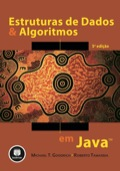
\includegraphics[height=0.3\paperheight]{imagens/livro_goodrich.jpg}
\end{figure}
\end{column}
%\vspace{3mm}
\begin{column}{0.85\linewidth}
\tiny{\textbf{Capítulo 7, Seções 7.1, 7.2, 7.3, 10.1, 10.2 e 10.5}\\
~}\\
\scriptsize{GOODRICH, Michael T.; TAMASSIA, Roberto. \textbf{Estruturas de dados e algoritmos em Java}. Tradução: Bernardo Copstein. 5. ed. Porto Alegre: Bookman, 2013. xxii, 713 p. E-book. ISBN 9788582600191. Tradução de: Data Structures and Algorithms in Java, 5th Edition. Disponível em: \textless{}\url{https://integrada.minhabiblioteca.com.br/\#/books/9788582600191/}\textgreater{}. Acesso em: 01 ago. 2023.}
\end{column}
\end{columns}

\end{frame}

%=======================================================
\section{Conceitos e Terminologia}

%-------------------------------------------------------
\begin{frame}\frametitle{Árvores}
\begin{itemize}
	\item Estruturas de dados não lineares
	\item Permitem a implementação de vários algoritmos mais rápidos do que no uso de estruturas de dados lineares como as listas
	\item Fornecem uma forma natural de organizar os dados
	\begin{itemize}
		\item Sistemas de arquivos
		\item Bancos de dados
		\item Sites da Web
	\end{itemize}
\end{itemize}
\end{frame}

%-------------------------------------------------------
\begin{frame}\frametitle{Árvore}
\begin{itemize}
	\item Tipo abstrato de dados que armazena elementos de maneira \textbf{hierárquica}
	\item Normalmente, são desenhadas colocando-se os elementos dentro de elipses ou retângulos e conectando-os com linhas retas
\begin{figure}[h]
	\centering
	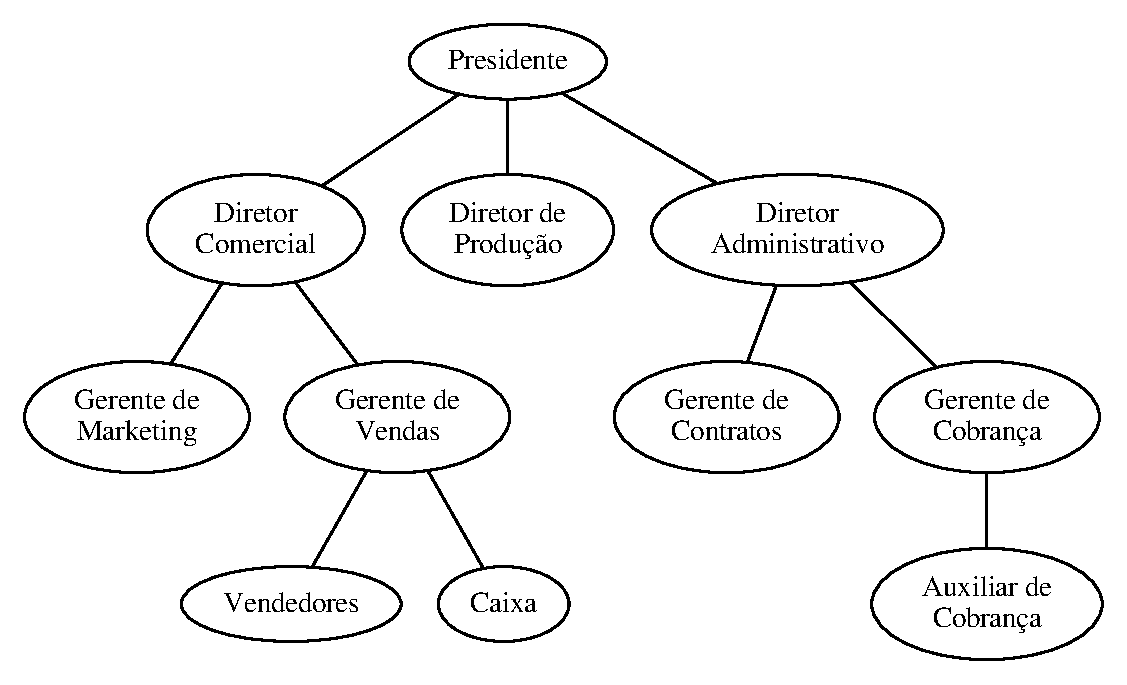
\includegraphics[height=0.55\paperheight]{imagens/arvore1.eps}
\end{figure}
\end{itemize}
\end{frame}

%-------------------------------------------------------
\begin{frame}\frametitle{Definição}
\begin{itemize}
	\item Formalmente uma árvore \textbf{T} é definida como um conjunto finito de um ou mais \textbf{nodos}, com a seguinte propriedade:
	\begin{itemize}
		\item Se \textbf{T} não é vazia, existe um nodo denominado \textbf{raiz} da árvore
		\item Os demais nodos formam $m > 0$ conjuntos disjuntos $S_1$, $S_2$, ..., $S_m$, sendo cada um destes conjuntos uma árvore
		\item As árvores $S_i$ ($1 \le i \le m$) são chamadas de \textbf{subárvores}
	\end{itemize}
	\item Pela definição
	\begin{itemize}
		\item Cada nodo da árvore é a raiz de uma subárvore
	\end{itemize}
\end{itemize}
\end{frame}

%-------------------------------------------------------
\begin{frame}\frametitle{Definição}
\begin{itemize}
	\item Portanto, uma árvore pode ser representada da seguinte forma:
\begin{figure}[h]
	\centering
	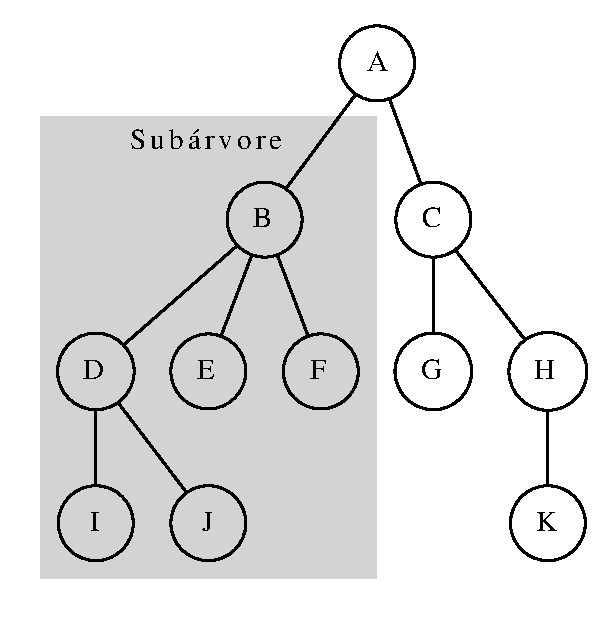
\includegraphics[height=0.60\paperheight]{imagens/arvore2.eps}
\end{figure}
	\item \textbf{A} é a raiz da árvore
\end{itemize}
\end{frame}

%-------------------------------------------------------
\begin{frame}\frametitle{Relacionamentos entre nodos	}
\begin{itemize}
	\item Outra propriedade de uma árvore \textbf{T}:
	\begin{itemize}
		\item Cada nodo \textbf{v} de \textbf{T} diferente da raiz tem um único nodo \textbf{pai}, \textbf{w}
		\item Todo nodo com \textbf{pai} \textbf{w} é \textbf{filho} de \textbf{w}
	\end{itemize}
	\item Pela definição
	\begin{itemize}
		\item Uma árvore pode ser vazia, isto é, não possui nodos
		\item Esta convenção permite que se defina uma árvore recursivamente
		\begin{itemize}
			\item Uma árvore \textbf{T} ou está vazia, ou consiste de um nodo \textbf{r}, chamado de raiz de \textbf{T}, e um conjunto de árvores cujas raízes são filhas de \textbf{r}
		\end{itemize}
	\end{itemize}
\end{itemize}
\end{frame}
	
%-------------------------------------------------------
\begin{frame}\frametitle{Relacionamentos entre nodos}
\begin{itemize}
	\item Outros relacionamentos entre nodos
	\begin{itemize}
		\item Dois nodos que são filhos de um mesmo pai são \textbf{irmãos}
		\item Um nodo \textbf{v} é \textbf{externo} se \textbf{v} não tem filhos
		\item Um nodo \textbf{v} é \textbf{interno} se tem um ou mais filhos
	\end{itemize}
	\item Nodo \textbf{interno} também é conhecido como \textbf{galho}
	\item Nodo \textbf{externo} também é conhecido como \textbf{folha}
\end{itemize}
\end{frame}

%-------------------------------------------------------
\begin{frame}\frametitle{Relacionamentos entre nodos}
\begin{itemize}
	\item A raiz de uma árvore é chamada de \textbf{pai} de suas subárvores
	\item As raízes das subárvores de um nodo são chamadas de \textbf{irmãos}, que, por sua vez, são \textbf{filhos} de seu nodo pai
\begin{columns}[T]
\begin{column}{0.5\linewidth}
%\vspace{-3mm}
\begin{figure}[h]
	\centering
	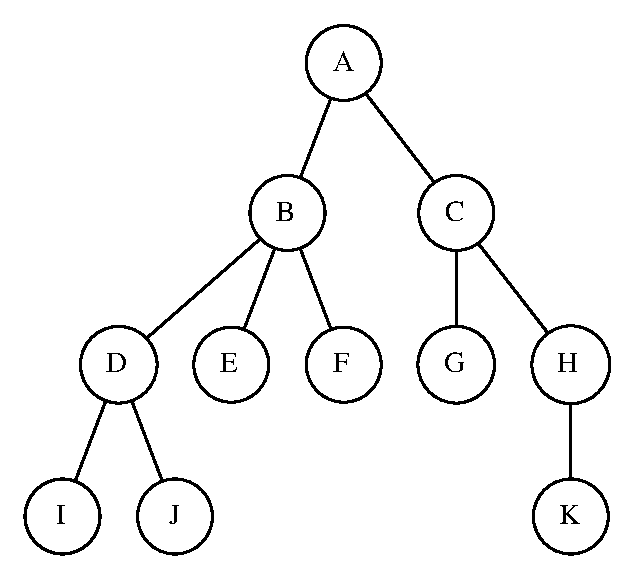
\includegraphics[height=0.55\paperheight]{imagens/arvore3.eps}
\end{figure}
\end{column}
\begin{column}{0.5\linewidth}
%\vspace{3mm}
\begin{itemize}
	\item \textbf{A} é pai de \textbf{B} e \textbf{C}
	\item \textbf{D}, \textbf{E} e \textbf{F} são irmãos
	\item \textbf{I} é filho de \textbf{J}
\end{itemize}
\end{column}
\end{columns}
\end{itemize}
\end{frame}

%-------------------------------------------------------
\begin{frame}\frametitle{``Árvore Invertida''}
\begin{figure}[h]
	\centering
	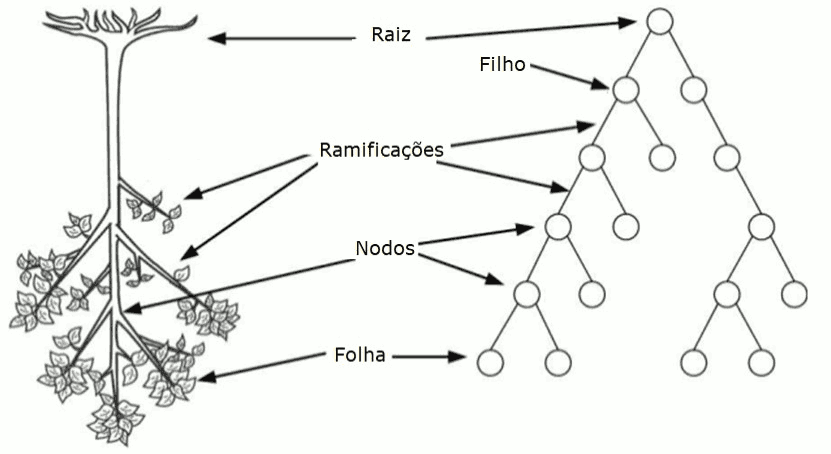
\includegraphics[height=0.60\paperheight]{imagens/arvore_invertida.png}\\
{\tiny Fonte: \url{https://di.ubi.pt/~cbarrico/Disciplinas/AlgoritmosEstruturasDadosLEI/Downloads/Teorica_ConceitosGeraisArvores.pdf}}
\end{figure}
\end{frame}

%-------------------------------------------------------
\begin{frame}\frametitle{Exemplo}
\begin{columns}[T]
\begin{column}{0.4\linewidth}
%\vspace{-3mm}
\begin{itemize}
	\item Organização hierárquica dos arquivos nos sistemas operacionais é uma árvore
	\item Nodos internos, neste caso, são associados a diretórios, e nodos externos a arquivos
	\item No Linux o diretório raiz é ``/''
\end{itemize}
\end{column}
\begin{column}{0.6\linewidth}
\vspace{-5mm}
\begin{figure}[h]
	\centering
	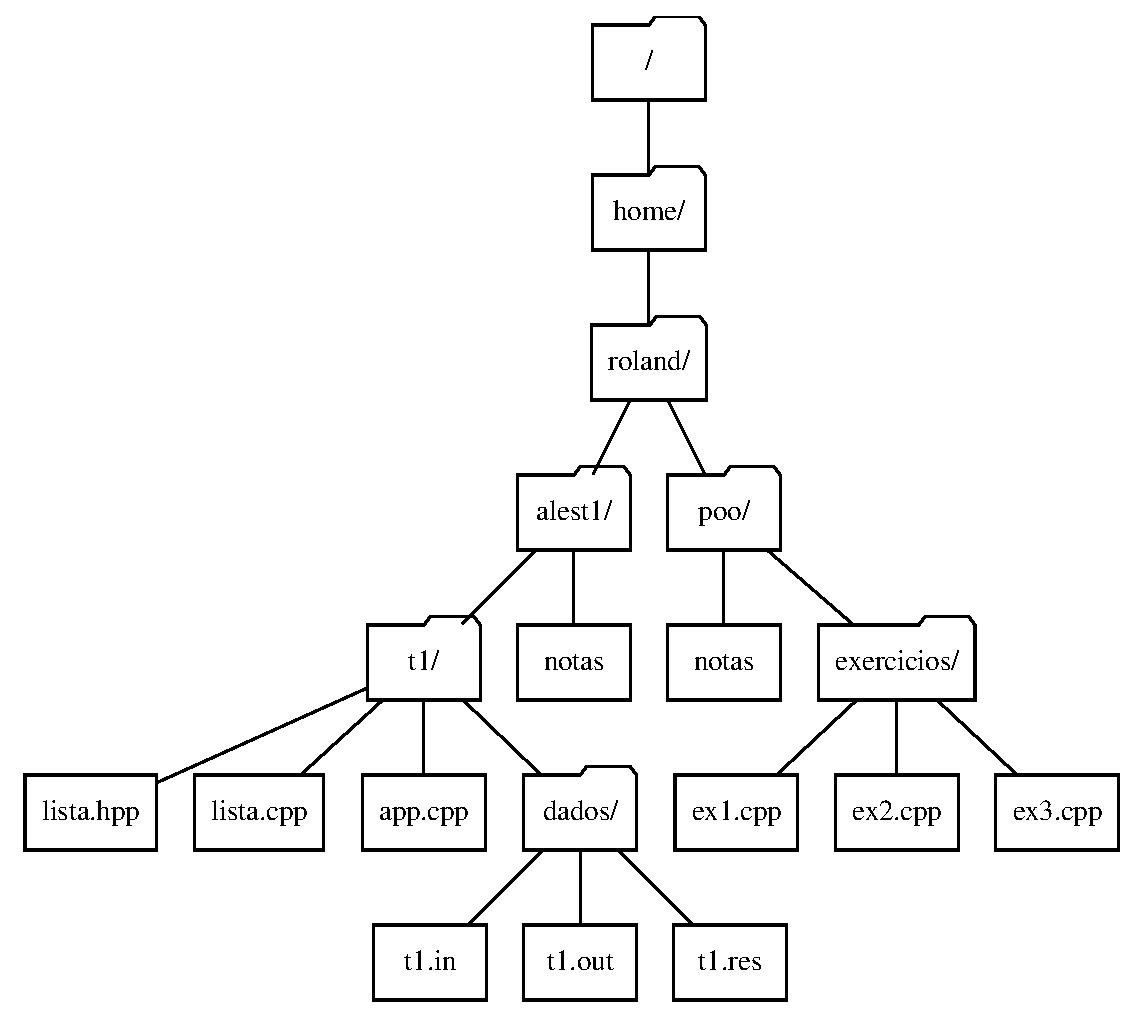
\includegraphics[height=0.7\paperheight]{imagens/arvore4.eps}
\end{figure}
\end{column}
\end{columns}
\end{frame}

%-------------------------------------------------------
\begin{frame}\frametitle{Arestas e Caminhos em Árvores}
\begin{columns}[T]
\begin{column}{0.4\linewidth}
%\vspace{-3mm}
\begin{itemize}
	\item Uma \textbf{\underline{aresta}} de uma árvore \textbf{T} é um par de nodos (\textbf{u},\textbf{v}) tal que \textbf{u} é pai de \textbf{v}, ou vice-versa
	\item Um \textbf{\underline{caminho}} de \textbf{T} é uma sequência de nodos tais que quaisquer dois nodos consecutivos
da sequência formam uma aresta
	\item Exemplo: \texttt{alest1/}, \texttt{t1/}, \texttt{dados/} e \texttt{t1.out} formam um caminho
\end{itemize}
\end{column}
\begin{column}{0.6\linewidth}
\vspace{-5mm}
\begin{figure}[h]
	\centering
	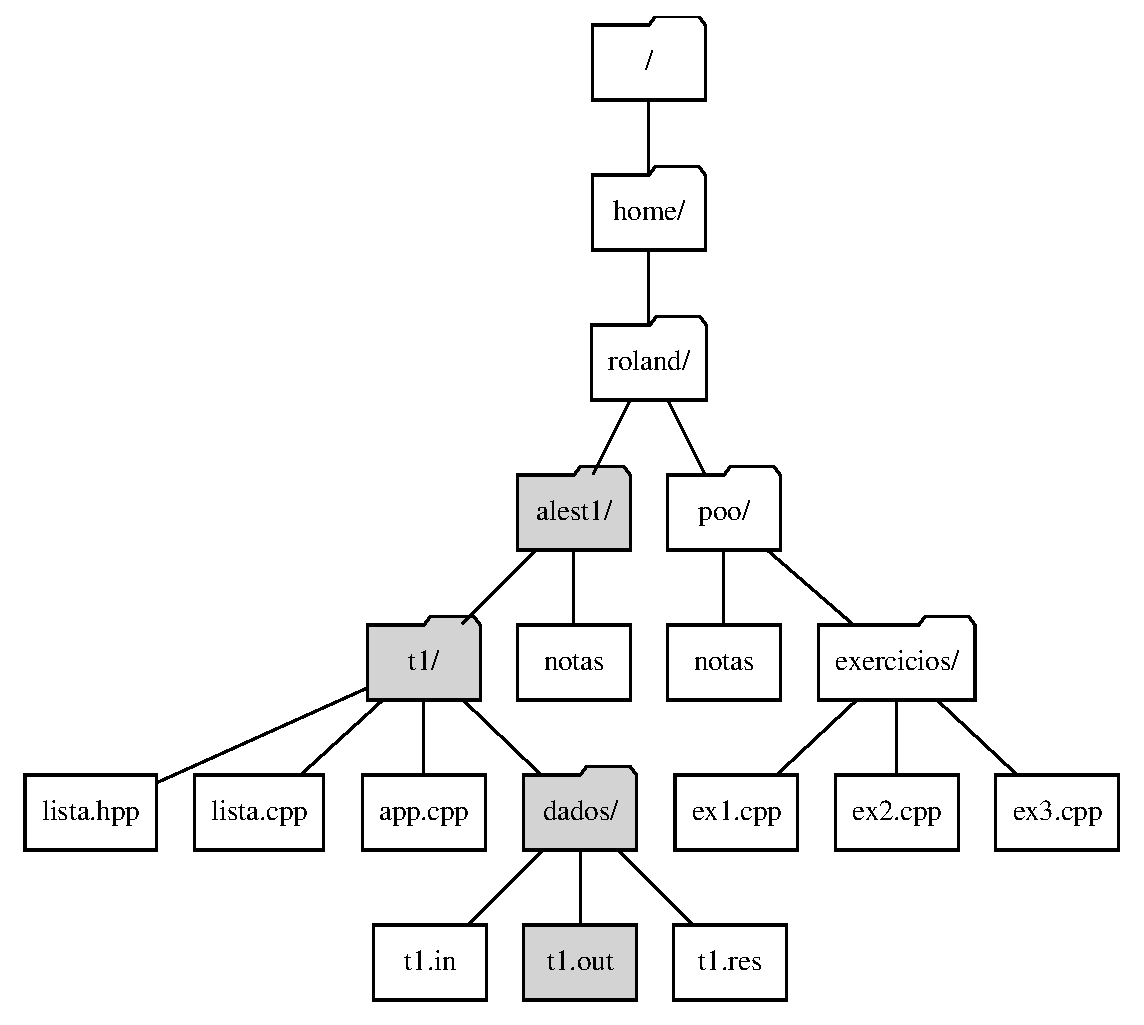
\includegraphics[height=0.7\paperheight]{imagens/arvore4-v2.eps}
\end{figure}
\end{column}
\end{columns}
\end{frame}

%-------------------------------------------------------
\begin{frame}\frametitle{Grau, Nível e Altura}
\begin{itemize}
	\item  Grau
	\begin{itemize}
		\item É o número de subárvores de um nodo
		\item Quando o grau é zero, ou seja, o nodo não possui filhos, ele é \textbf{folha}
	\end{itemize}
	\item Nível de um nodo
	\begin{itemize}
		\item É o número de linhas que liga o nodo à raiz, sabendo que a raiz é o nível zero
	\end{itemize}
	\item Altura
	\begin{itemize}
		\item É definida como sendo o nível mais alto da árvore
	\end{itemize}
\end{itemize}
\end{frame}

%-------------------------------------------------------
\begin{frame}\frametitle{Grau, Nível e Altura}
\begin{columns}[T]
\begin{column}{0.4\linewidth}
%\vspace{-3mm}
\begin{itemize}
	\item Grau:
	\begin{itemize}
		\item Nodo A:
		\item Nodo B:
		\item Nodo C:
		\item Nodo D:
		\item Nodo E:
		\item Nodo F:
		\item Nodo G:
		\item Nodo H:
		\item Nodo I:
		\item Nodo J:
		\item Nodo K:
	\end{itemize}
\end{itemize}
\end{column}
\begin{column}{0.6\linewidth}
\vspace{-5mm}
\begin{figure}[h]
	\centering
	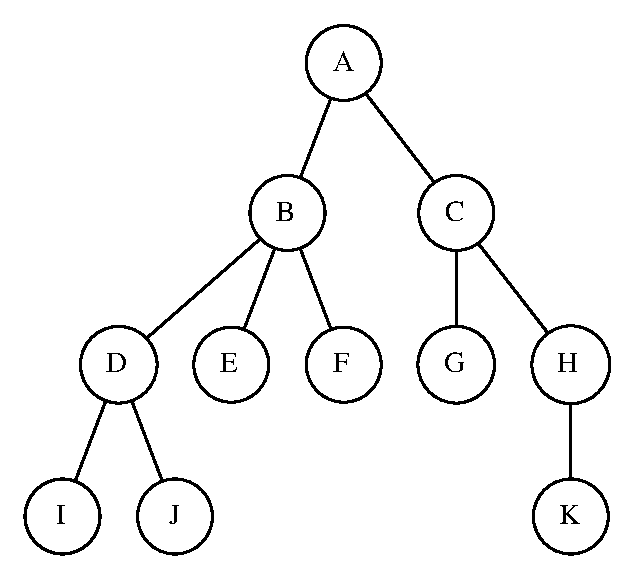
\includegraphics[height=0.70\paperheight]{imagens/arvore3.eps}
\end{figure}
\end{column}
\end{columns}
\end{frame}

%-------------------------------------------------------
\begin{frame}\frametitle{Grau, Nível e Altura}
\begin{columns}[T]
\begin{column}{0.4\linewidth}
%\vspace{-3mm}
\begin{itemize}
	\item Grau:
	\begin{itemize}
		\item Nodo A: 2
		\item Nodo B: 3
		\item Nodo C: 2
		\item Nodo D: 2
		\item Nodo E: 0
		\item Nodo F: 0
		\item Nodo G: 0
		\item Nodo H: 1
		\item Nodo I: 0
		\item Nodo J: 0
		\item Nodo K: 0
	\end{itemize}
\end{itemize}
\end{column}
\begin{column}{0.6\linewidth}
\vspace{-5mm}
\begin{figure}[h]
	\centering
	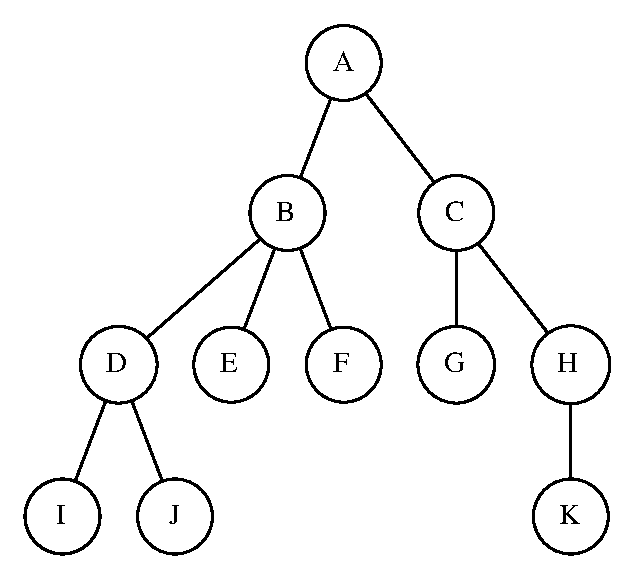
\includegraphics[height=0.70\paperheight]{imagens/arvore3.eps}
\end{figure}
\end{column}
\end{columns}
\end{frame}

%-------------------------------------------------------
\begin{frame}\frametitle{Grau, Nível e Altura}
\begin{columns}[T]
\begin{column}{0.4\linewidth}
%\vspace{-3mm}
\begin{itemize}
	\item Nível:
	\begin{itemize}
		\item Nodo A:
		\item Nodo B:
		\item Nodo C:
		\item Nodo D:
		\item Nodo E:
		\item Nodo F:
		\item Nodo G:
		\item Nodo H:
		\item Nodo I:
		\item Nodo J:
		\item Nodo K:
	\end{itemize}
	\item Altura:
	\begin{itemize}
		\item Árvore:
	\end{itemize}
\end{itemize}
\end{column}
\begin{column}{0.6\linewidth}
\vspace{-5mm}
\begin{figure}[h]
	\centering
	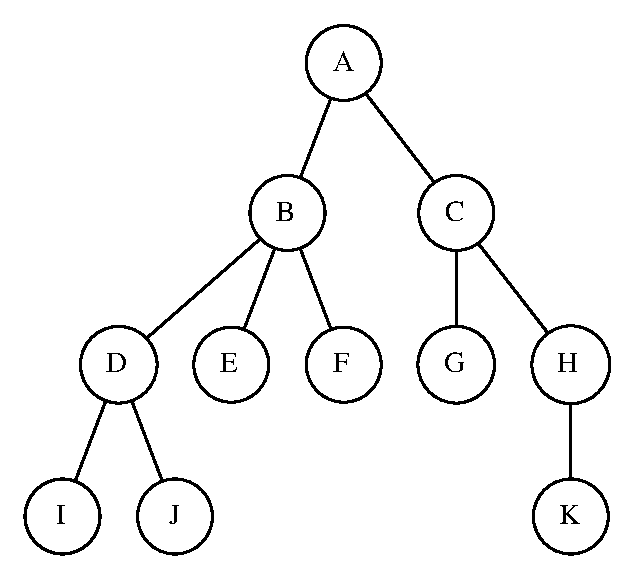
\includegraphics[height=0.70\paperheight]{imagens/arvore3.eps}
\end{figure}
\end{column}
\end{columns}
\end{frame}

%-------------------------------------------------------
\begin{frame}\frametitle{Grau, Nível e Altura}
\begin{columns}[T]
\begin{column}{0.4\linewidth}
%\vspace{-3mm}
\begin{itemize}
	\item Nível:
	\begin{itemize}
		\item Nodo A: 0
		\item Nodo B: 1
		\item Nodo C: 1
		\item Nodo D: 2
		\item Nodo E: 2
		\item Nodo F: 2
		\item Nodo G: 2
		\item Nodo H: 2
		\item Nodo I: 3
		\item Nodo J: 3
		\item Nodo K: 3
	\end{itemize}
	\item Altura:
	\begin{itemize}
		\item Árvore: 3
	\end{itemize}
\end{itemize}
\end{column}
\begin{column}{0.6\linewidth}
\vspace{-5mm}
\begin{figure}[h]
	\centering
	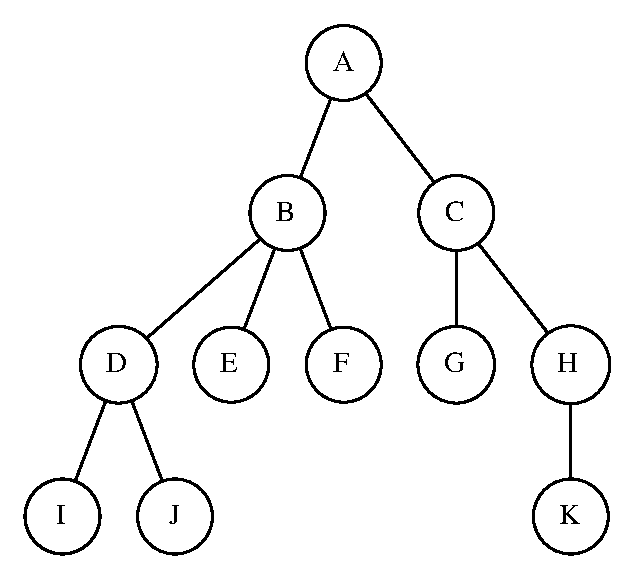
\includegraphics[height=0.70\paperheight]{imagens/arvore3.eps}
\end{figure}
\end{column}
\end{columns}
\end{frame}

%-------------------------------------------------------
\begin{frame}\frametitle{Grau, Nível e Altura}
\begin{columns}[T]
\begin{column}{0.4\linewidth}
%\vspace{-3mm}
\begin{itemize}
	\item Raiz: A
	\item Nodos internos: B, C, D, H
	\item Folhas: I, J, E, F, G, K
	\end{itemize}
\end{column}
\begin{column}{0.6\linewidth}
\vspace{-5mm}
\begin{figure}[h]
	\centering
	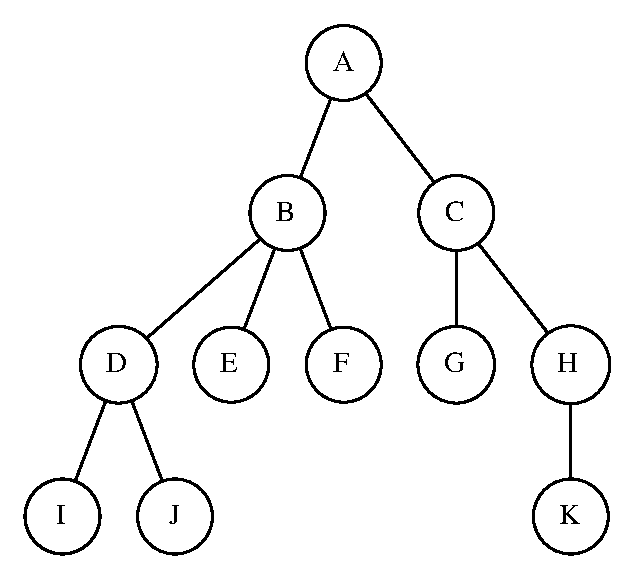
\includegraphics[height=0.70\paperheight]{imagens/arvore3.eps}
\end{figure}
\end{column}
\end{columns}
\end{frame}

%-------------------------------------------------------
\begin{frame}\frametitle{Floresta}
\begin{itemize}
	\item Conjunto de uma ou mais árvores disjuntas
	\item Se eliminarmos o nodo raiz de uma árvore, obtém-se uma floresta
	\item Os filhos da raiz original irão se transformar nas raízes das novas árvores
\end{itemize}
\begin{figure}[h]
	\centering
	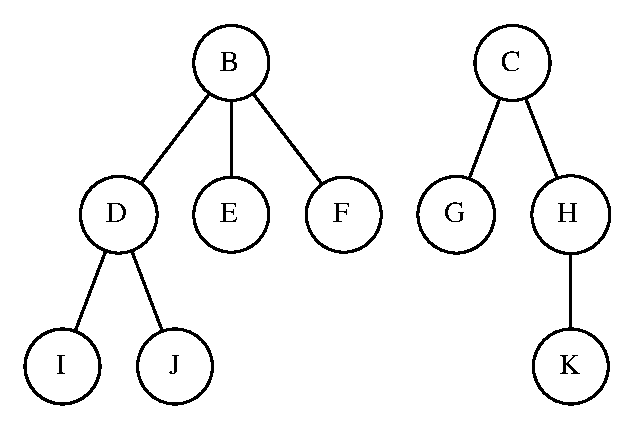
\includegraphics[height=0.5\paperheight]{imagens/floresta.eps}
\end{figure}
\end{frame}

%=======================================================
\section{Exercícios}

%-------------------------------------------------------
\begin{frame}[fragile]\frametitle{Exercício 1}
\begin{enumerate}
        \setcounter{enumi}{0}
\item Analise a árvore abaixo.
\begin{columns}[T]
\begin{column}{0.5\linewidth}
%\vspace{-5mm}
\begin{figure}[h]
	\centering
	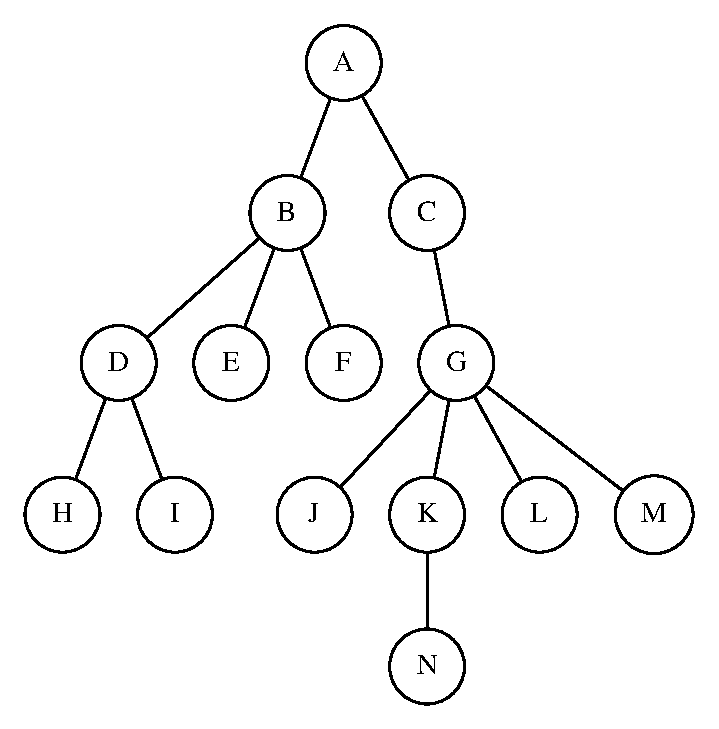
\includegraphics[height=0.6\paperheight]{imagens/exercicio01.eps}
\end{figure}
\end{column}
\begin{column}{0.5\linewidth}
E responda:
\begin{itemize}
	\item Qual é a altura da árvore?\\
	\item Quais são as folhas da árvore?\\
	\item Quais são os nodos irmãos?\\
	\item Os nodos D e G são pais de que nodos?\\
	\item Qual é o grau do nodo B?\\
	\item Qual é o grau do nodo G?\\
	\item Quais são os níveis dos nodos B, G, H, L e N?\\
\end{itemize}
\end{column}
\end{columns}
\end{enumerate}
\end{frame}

%-------------------------------------------------------
\begin{frame}[fragile]\frametitle{Exercício 2}
\begin{enumerate}
        \setcounter{enumi}{1}
\item Analise a árvore abaixo.
\begin{columns}[T]
\begin{column}{0.5\linewidth}
%\vspace{-5mm}
\begin{figure}[h]
	\centering
	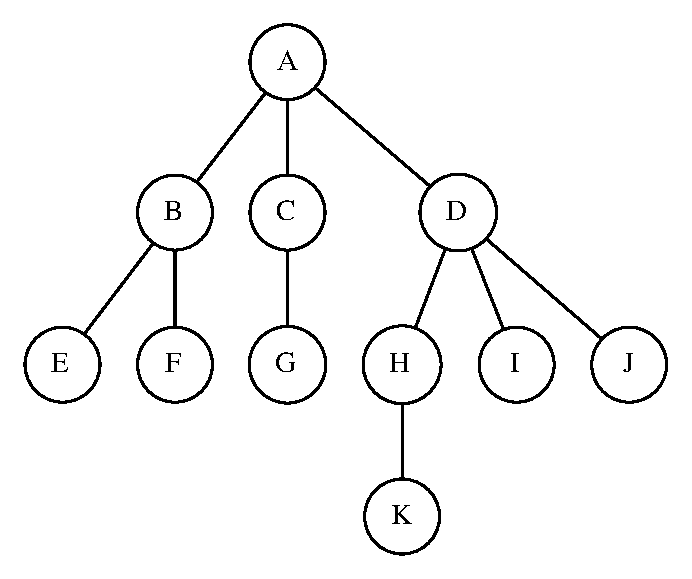
\includegraphics[height=0.5\paperheight]{imagens/exercicio02.eps}
\end{figure}
\end{column}
\begin{column}{0.5\linewidth}
E responda:
\begin{itemize}
	\item Qual é a altura da árvore?\\
	\item Quais são as folhas da árvore?\\
	\item Quais são os nodos irmãos?\\
	\item Quais são os nodos internos?
	\item Qual é o grau do nodo C?
	\item Qual é o grau do nodo D?
	\item Quais são os níveis dos nodos C, H e K?
\end{itemize}
\end{column}
\end{columns}
\end{enumerate}
\end{frame}

%=======================================================
\section{Aplicações}

%-------------------------------------------------------
\begin{frame}\frametitle{Aplicações}
\begin{itemize}
	\item Árvores são estruturas de dados adequadas para representar diversos tipos de informações
	\item Várias aplicações que podem utilizar árvores
\end{itemize}
\end{frame}

%-------------------------------------------------------
\begin{frame}\frametitle{Árvore de decisão}
\begin{itemize}
	\item Exemplo: Ir ou não ir para praia?
\begin{figure}[h]
	\centering
	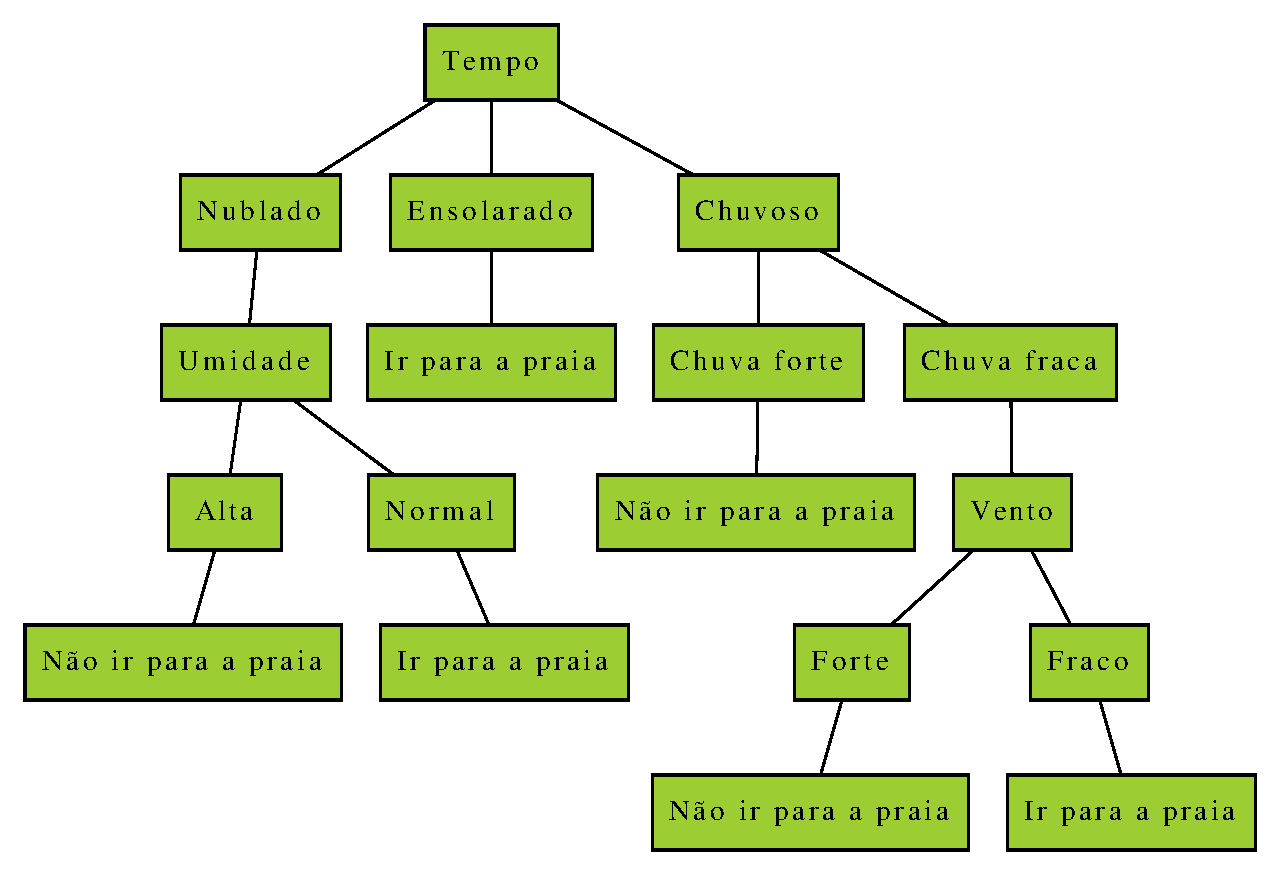
\includegraphics[height=0.65\paperheight]{imagens/arvore_de_decisao.eps}
\end{figure}
\end{itemize}
\end{frame}

%-------------------------------------------------------
\begin{frame}\frametitle{Representação de estruturas/informações hierárquicas}
\begin{itemize}
	\item Árvore genealógica
	\item Organização de livros e documentos
	\item Organização hierárquica de cargos de uma empresa
	\item Sistemas de arquivos
\begin{figure}[h]
	\centering
	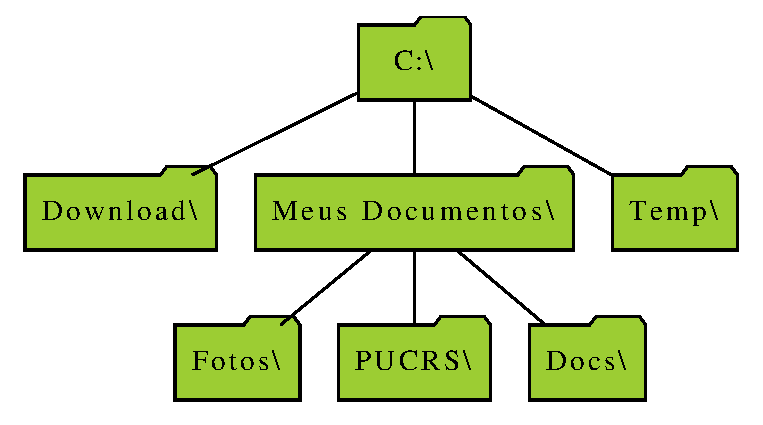
\includegraphics[height=0.4\paperheight]{imagens/arvore_de_diretorios.eps}
\end{figure}
\end{itemize}
\end{frame}

%-------------------------------------------------------
\begin{frame}[fragile]\frametitle{Representação de estruturas/informações hierárquicas}
\begin{itemize}
	\item Arquivos HTML e XML
\begin{lstlisting}[language=XML,basicstyle=\ttfamily\scriptsize]
<?xml version="1.0"?>
<Company>
  <Employee>
    <FirstName>Maria</FirstName>
    <LastName>Silva</LastName>
    <PhoneNumber>(51)98986767</PhoneNumber>
    <Email>maria.silva@gmail.com</Email>
    <Address>
      <Street>Rua dos Andradas 1586/202</Street>
      <City>Porto Alegre</City>
      <State>RS</State>
      <Zip>90021-212</Zip>
    </Address>
  </Employee>
</Company>
\end{lstlisting}
\end{itemize}
\end{frame}

%-------------------------------------------------------
\begin{frame}\frametitle{Computação Gráfica}
\begin{columns}[T]
\begin{column}{0.30\linewidth}
\begin{itemize}
	\item Grafo de cena
\end{itemize}
\begin{figure}[h]
	\centering
	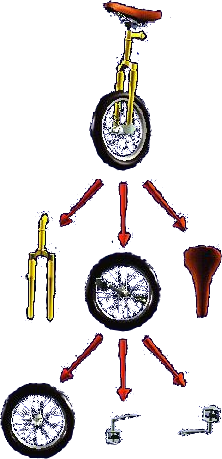
\includegraphics[height=0.60\paperheight]{imagens/grafo_de_cena.png}
\end{figure}
\end{column}
\begin{column}{0.70\linewidth}
\begin{itemize}
	\item Algoritmos para remoção de superfícies escondidas (árvore \emph{Binary Space-Partitioning})
\end{itemize}
\begin{figure}[h]
	\centering
	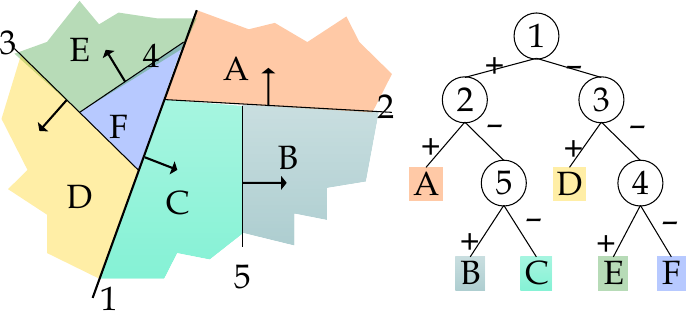
\includegraphics[height=0.50\paperheight]{imagens/binary_space_partitioning.png}
\end{figure}
\end{column}
\end{columns}
\end{frame}

%-------------------------------------------------------
\begin{frame}\frametitle{Computação Gráfica}
\begin{itemize}
	\item Representação de objetos (Quadtree e Octree), etc.
\end{itemize}
\begin{columns}[T]
\begin{column}{0.36\linewidth}
\begin{figure}[h]
	\centering
	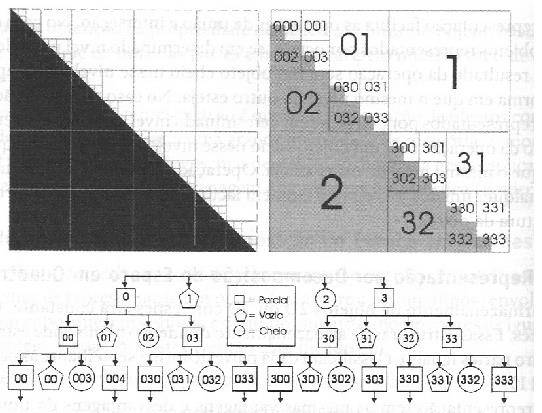
\includegraphics[height=0.45\paperheight]{imagens/quadtree.jpg}
\end{figure}
\end{column}
\begin{column}{0.34\linewidth}
\begin{figure}[h]
	\centering
	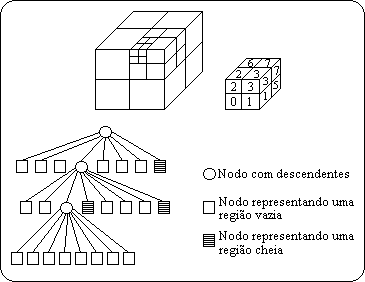
\includegraphics[height=0.45\paperheight]{imagens/octree.png}
\end{figure}
\end{column}
\begin{column}{0.30\linewidth}
\begin{figure}[h]
	\centering
	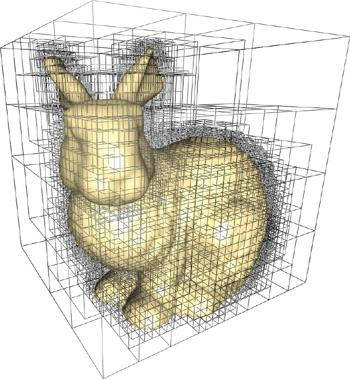
\includegraphics[height=0.45\paperheight]{imagens/coelho.jpg}
\end{figure}
\end{column}
\end{columns}
\end{frame}

%-------------------------------------------------------
\begin{frame}\frametitle{Eliminatórias de Campeonatos}
\begin{figure}[h]
	\centering
	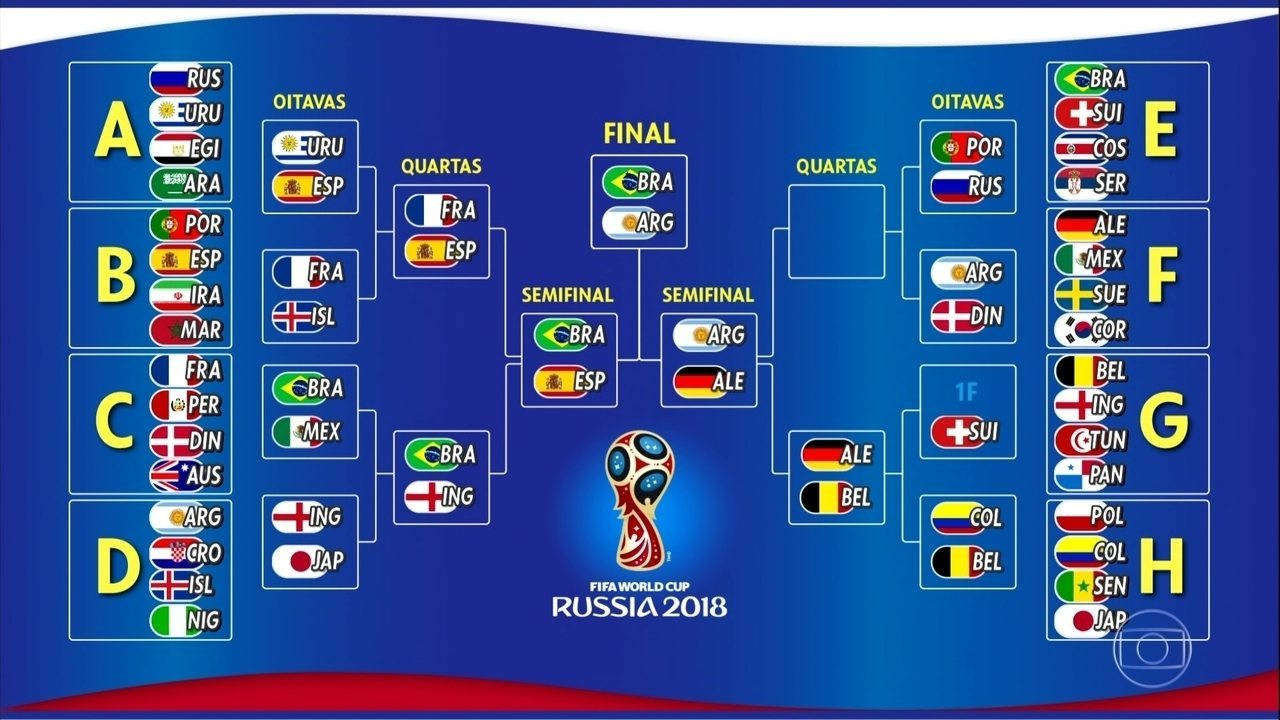
\includegraphics[height=0.70\paperheight]{imagens/copa_russia_2018.jpg}
\end{figure}
\end{frame}

%-------------------------------------------------------
\begin{frame}\frametitle{Interfaces Gráficas com o Usuário}
\begin{columns}[T]
\begin{column}{0.62\linewidth}
\vspace{-5mm}
\begin{figure}[h]
	\centering
	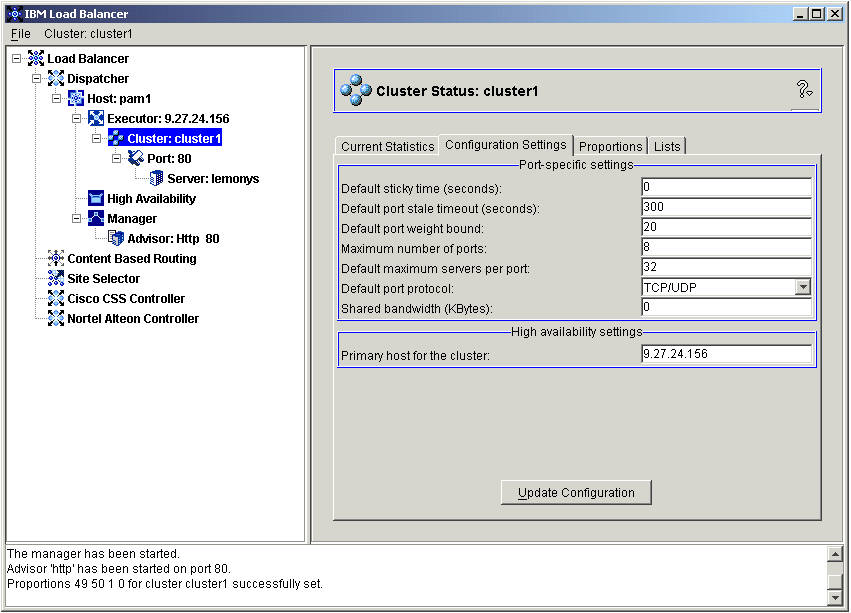
\includegraphics[height=0.70\paperheight]{imagens/interface1.jpg}
\end{figure}
\end{column}
\begin{column}{0.38\linewidth}
\vspace{-5mm}
\begin{figure}[h]
	\centering
	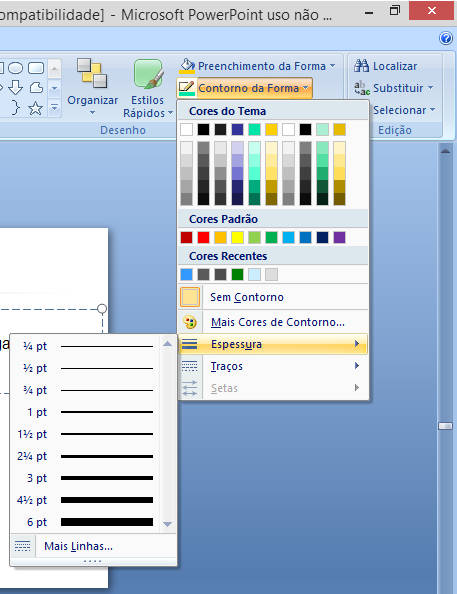
\includegraphics[height=0.70\paperheight]{imagens/interface2.jpg}
\end{figure}
\end{column}
\end{columns}
\end{frame}

%-------------------------------------------------------
\begin{frame}\frametitle{Expressões Aritméticas}
\begin{itemize}
	\item Pode-se usar árvores para representar e avaliar expressões aritméticas
	\item Exemplo: \texttt{A * B + C / ( D + E )}
\begin{figure}[h]
	\centering
	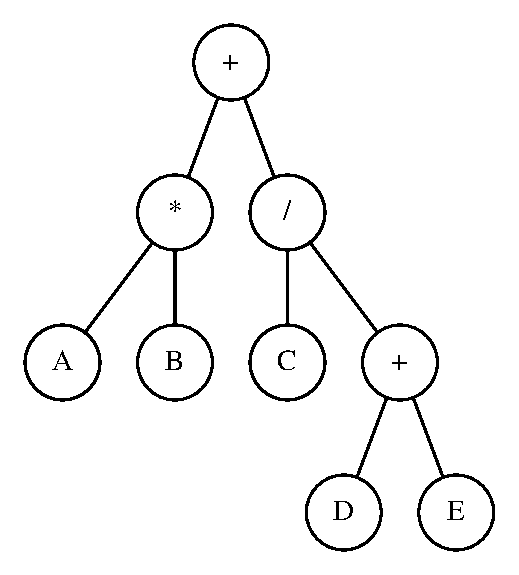
\includegraphics[height=0.6\paperheight]{imagens/expressao_aritmetica.eps}
\end{figure}
\end{itemize}
\end{frame}

%-------------------------------------------------------
\begin{frame}\frametitle{Organização das Páginas de um \emph{Site}}
\vspace{-3mm}
\begin{figure}[h]
	\centering
	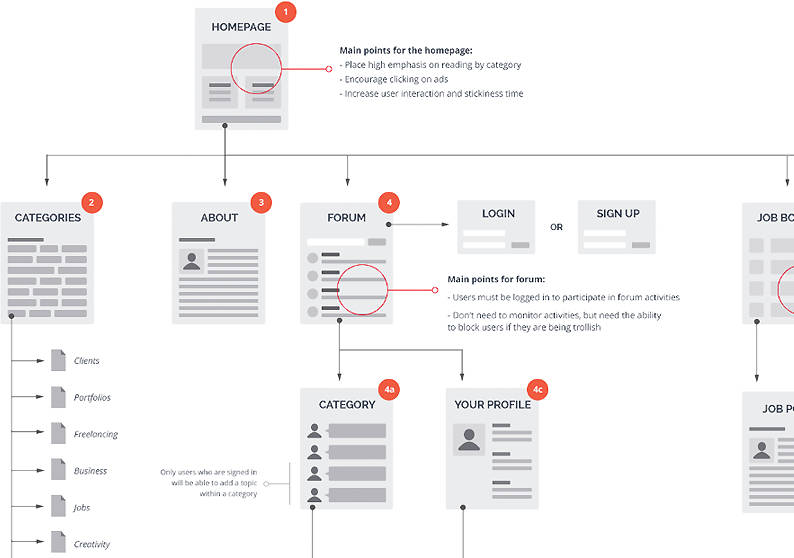
\includegraphics[height=0.70\paperheight]{imagens/paginas_web.jpg}\\
{\tiny Fonte: \url{https://dribbble.com/shots/1198252-Sitemap-For-Student-Guide}}
\end{figure}	
\end{frame}

	
%=======================================================
\section{Representação na Memória}

%-------------------------------------------------------
\begin{frame}\frametitle{Representação na Memória}
\begin{itemize}
	\item Da mesma forma que as estruturas de dados lineares, podemos alocar as árvores de duas maneiras
	\begin{itemize}
		\item Por contiguidade
		\item Por encadeamento
	\end{itemize}
\end{itemize}
\end{frame}

%-------------------------------------------------------
\begin{frame}[fragile]\frametitle{Representação por Contiguidade}
\begin{itemize}
	\item A árvore é armazenada em um arranjo
	\item Cada posição por arranjo pode, por exemplo, conter, além da informação do nodo, referências aos nodos filhos
\begin{columns}[T]
\begin{column}{0.30\linewidth}
%\vspace{-5mm}
\begin{figure}[h]
	\centering
	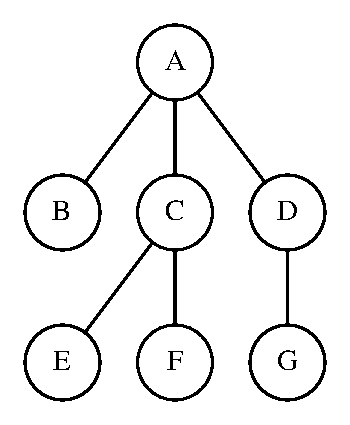
\includegraphics[height=0.4\paperheight]{imagens/arvore_a.eps}
\end{figure}
\end{column}
\begin{column}{0.70\linewidth}
\begin{figure}[h]
	\centering
	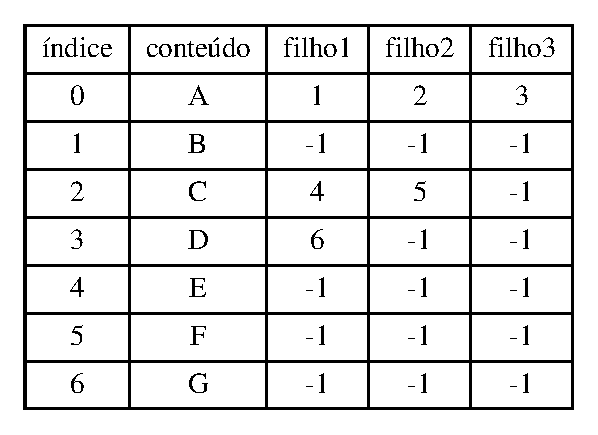
\includegraphics[height=0.4\paperheight]{imagens/arvore_a-cont.eps}
\end{figure}
\end{column}
\end{columns}
\end{itemize}
\end{frame}

%-------------------------------------------------------
\begin{frame}\frametitle{Representação por Contiguidade}
\begin{itemize}
	\item Vantagem:
	\begin{itemize}
		\item Forma de armazenar árvores em arquivos
	\end{itemize}
	\item Desvantagem:
	\begin{itemize}
		\item Quantidade de processamento para inserção, remoção ou mesmo localização de um nodo
	\end{itemize}
\end{itemize}
\end{frame}

%-------------------------------------------------------
\begin{frame}[fragile]\frametitle{Representação por Encadeamento}
\begin{itemize}
	\item Forma \textbf{mais usual}
	\item Facilita as operações de inserção, remoção e pesquisa na árvore
	\item Cada nodo conterá, além da informação, as referências das suas subárvores
\begin{columns}[T]
\begin{column}{0.30\linewidth}
%\vspace{-5mm}
\begin{figure}[h]
	\centering
	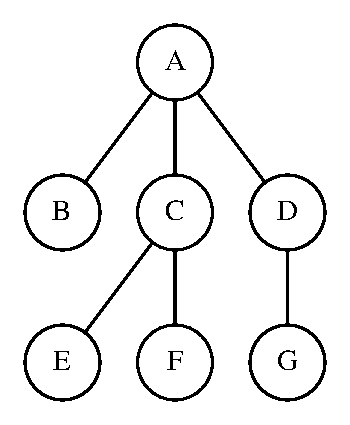
\includegraphics[height=0.4\paperheight]{imagens/arvore_a.eps}
\end{figure}
\end{column}
\begin{column}{0.70\linewidth}
\begin{figure}[h]
	\centering
	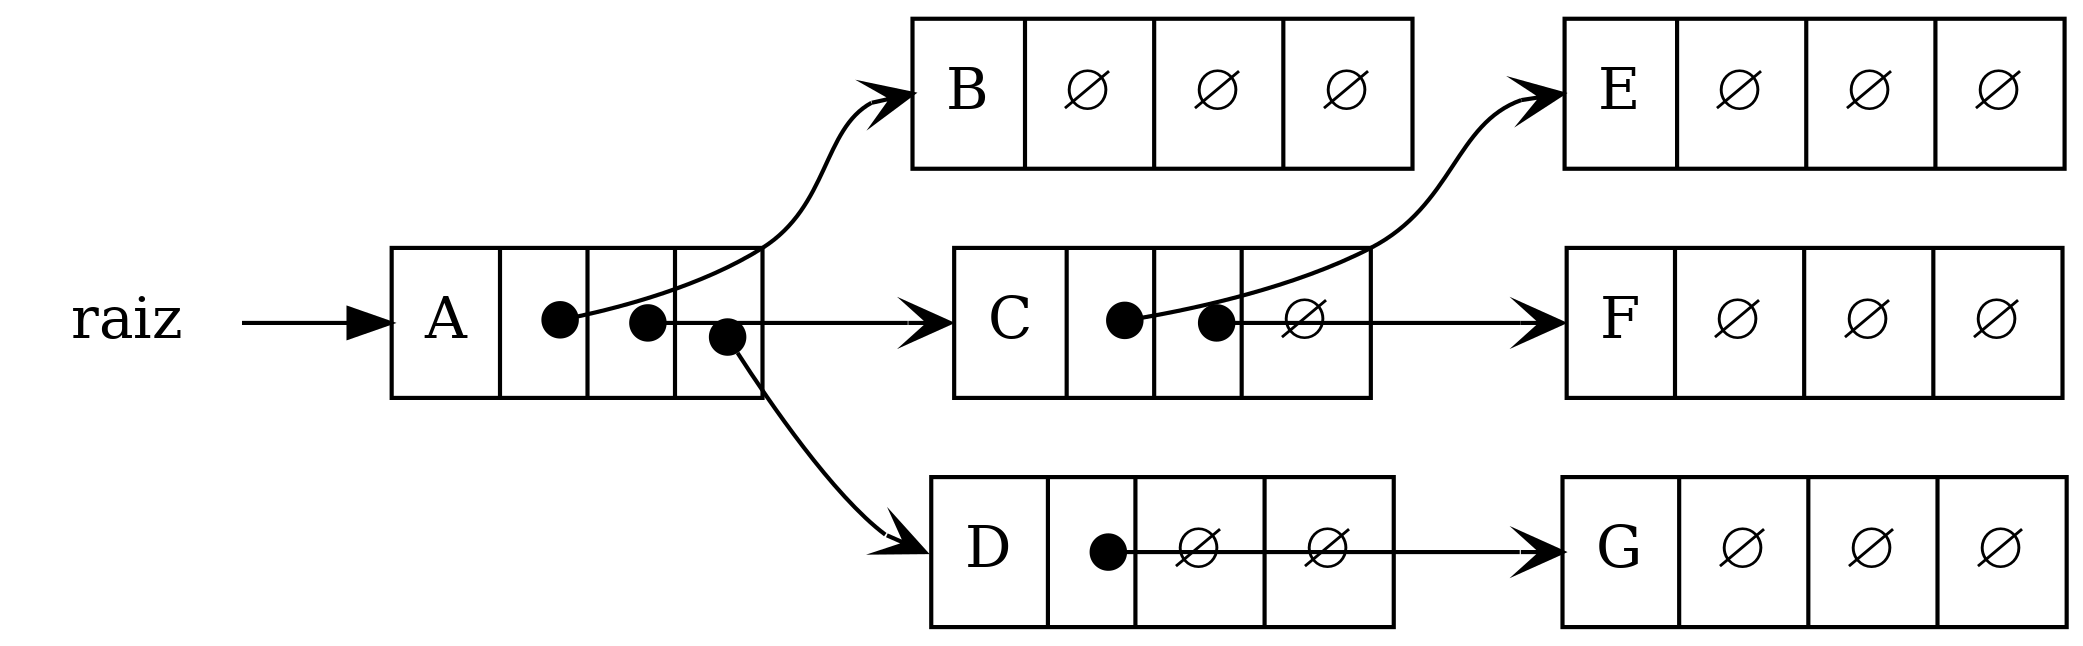
\includegraphics[height=0.35\paperheight]{imagens/arvore_a-enc.png}
\end{figure}
\end{column}
\end{columns}
\end{itemize}
\end{frame}

%-------------------------------------------------------
\begin{frame}\frametitle{Representação por Encadeamento}
\begin{itemize}
	\item  No caso de árvores ``genéricas'', cada nodo pode ter uma quantidade de subárvores diferentes
	\item Torna-se necessário:
	\begin{itemize}
		\item Limitar, ou seja, determinar o número máximo de subárvores que cada nodo deve conter
		\item Ou ter uma lista de subárvores
	\end{itemize}
	\item Isso é necessário, pois os nodos de uma mesma árvore são todos do mesmo tipo
\end{itemize}
\end{frame}

%-------------------------------------------------------
\begin{frame}\frametitle{Exemplo}
\begin{columns}[T]
\begin{column}{0.25\linewidth}
%\vspace{-5mm}
\begin{figure}[h]
	\centering
	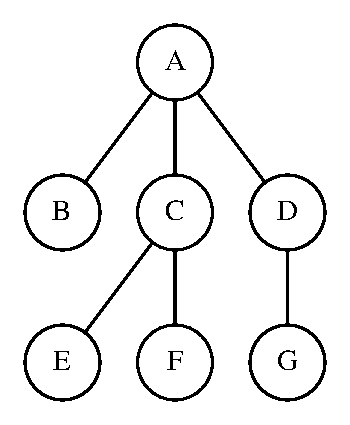
\includegraphics[height=0.4\paperheight]{imagens/arvore_a.eps}
\end{figure}
\end{column}
\begin{column}{0.75\linewidth}
\pause\lstinputlisting[basicstyle=\ttfamily\tiny]{src/exemplo01.cpp}
\end{column}
\end{columns}
\end{frame}

%-------------------------------------------------------
\begin{frame}\frametitle{GraphViz}
\vspace{-2mm}
\begin{figure}[h]
	\centering
	
\includegraphics[height=0.25\paperheight]{imagens/graphviz.png}
\end{figure}
\vspace{-3mm}
\begin{itemize}
	\item Graphviz (abreviação de \emph{Graph Visualization Software}) é uma ferramenta de código-fonte aberto para desenhar grafos (formados por nodos e arestas) especificados a partir de uma linguagem de escrite chamada DOT (que usa a extensão ``gv'')
	\item GraphViz também provê bibliotecas para que aplicações possam usar suas facilidades
	\item É um \emph{software} livre licenciado através da Licença Pública Eclipse
	\item Página: \url{https://graphviz.org/}
	\item Há várias opções para gerar imagens a partir dos arquivos no formato DOT
	\begin{itemize}
		\item \url{https://dreampuf.github.io/GraphvizOnline/}
	\end{itemize}
\end{itemize}
\end{frame}

%-------------------------------------------------------
\begin{frame}[fragile]\frametitle{GraphViz}
\begin{columns}[T]
\begin{column}{0.3\linewidth}
%\vspace{-5mm}
\textbf{\underline{Grafo:}}\\
\begin{figure}[h]
	\centering
	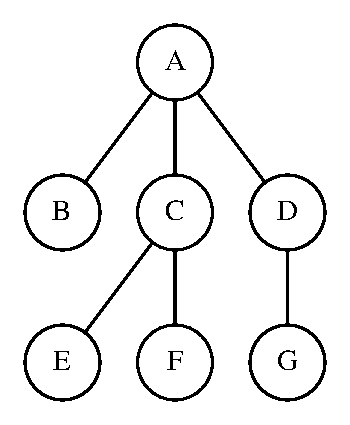
\includegraphics[height=0.4\paperheight]{imagens/arvore_a.eps}
\end{figure}
\end{column}
\begin{column}{0.35\linewidth}
\textbf{\underline{Versão 1:}}\\
\lstinputlisting[basicstyle=\ttfamily\tiny]{imagens/arvore_a.gv}
\end{column}
\begin{column}{0.35\linewidth}
\textbf{\underline{Versão 2:}}\\
\lstinputlisting[basicstyle=\ttfamily\tiny]{imagens/arvore_a-v2.gv}
\end{column}
\end{columns}
\end{frame}

%=======================================================
\section{Exercícios}

%-------------------------------------------------------
\begin{frame}[fragile]\frametitle{Exercício 3}
\begin{enumerate}
        \setcounter{enumi}{2}
	\small
	\item Considere a árvore e o programa que cria esta árvore correspondente, usando estruturas encadeadas em C++, ambos apresentados na próxima página. Observe que o nodo declarado (\texttt{struct Node}) armazena um caractere (\texttt{char}) e suporta até 3 subárvores (ou seja, cada nodo pode ter 3 nodos filhos). Para este programa, implemente as seguintes funções:
	\begin{itemize}
		\footnotesize
		\item \texttt{void clean(Node *root)}: que recebe o endereço de um nodo e faz a desalocação de todos os nodos da árvore a partir do nodo recebido (\texttt{root}) -- esta função deve ser implementada de forma recursiva;
		\item \texttt{string strGraphViz(Node *root)}: que recebe o endereço de um nodo e gera uma cadeia de caracteres (\texttt{string}) com representação da árvore no formato DOT, usado pelo GraphViz -- esta função deve: imprimir a parte inicial do formato DOT; chamar um outro método recursivo (por exemplo, \texttt{string strNode(Node *node)}) para gerar a lista de arestas entre os nodos; imprimir a parte final do formato DOT.
	\end{itemize}
	Rode o seu programa, por exemplo, com:
\begin{lstlisting}[basicstyle=\ttfamily\scriptsize,language=bash]
./exercicio03 > exercicio03.gv
\end{lstlisting}
	Use o site \url{https://dreampuf.github.io/GraphvizOnline/} para verificar se o arquivo \texttt{exercicio03.gv} foi corretamente gerado.
\end{enumerate}
\end{frame}

%-------------------------------------------------------
\begin{frame}[fragile]\frametitle{Exercício 3}
\begin{columns}
\begin{column}{0.23\linewidth}
%\vspace{-5mm}
\begin{figure}[h]
	\centering
	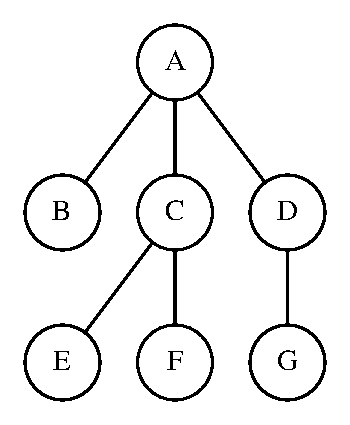
\includegraphics[height=0.4\paperheight]{imagens/arvore_a.eps}
\end{figure}
\end{column}
\begin{column}{0.77\linewidth}
\fontsize{6pt}{6pt}\selectfont{
\lstinputlisting{src/exercicio03.cpp}
}
\end{column}
\end{columns}
\end{frame}

%-------------------------------------------------------
\begin{frame}[fragile]\frametitle{Exercício 4}
\begin{enumerate}
        \setcounter{enumi}{3}
	\small
	\item Considere a árvore abaixo e, usando como modelo o código do exercício 3 (resolvido), implemente um programa em C++ que crie esta árvore em memória, que a imprima no formato DOT e que desaloque corretamente todos os nodos da árvore. Use o site \url{https://dreampuf.github.io/GraphvizOnline/} para verificar se o arquivo DOT foi corretamente gerado.
\begin{figure}[h]
	\centering
	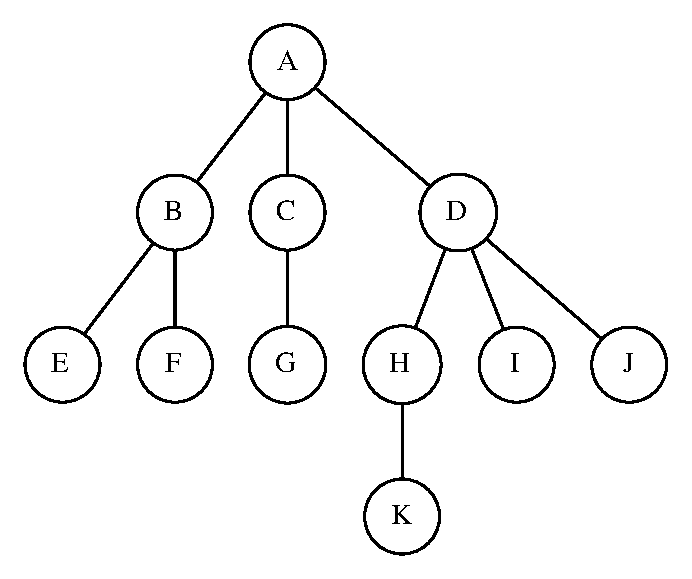
\includegraphics[height=0.5\paperheight]{imagens/exercicio02.eps}
\end{figure}
\end{enumerate}
\end{frame}

%=======================================================
\section{TAD para Árvore}

%-------------------------------------------------------
\begin{frame}\frametitle{TAD para Árvore}
\begin{itemize}
	\item Um TAD para árvore:
	\begin{itemize}
		\item Armazena elementos em nodos
		\item O posicionamento dos nodos satisfaz as relações pai-filho
		\item Operações consideram as propriedades desta estrutura de dados hierárquica
	\end{itemize}
\end{itemize}
\end{frame}

%-------------------------------------------------------
\begin{frame}\frametitle{TAD para Árvore}
\begin{itemize}
	\item Uma árvore deve disponibilizar métodos de acesso que retornam e aceitam posições:
	\begin{itemize}
		\item \texttt{root()}: retorna a raiz da árvore
		\item \texttt{parent(v)}: retorna o nodo pai de \texttt{v}, ocorrendo um erro se for a raiz
		\item \texttt{children(v)}: retorna os filhos do nodo \texttt{v}
	\end{itemize}
\end{itemize}
\end{frame}

%-------------------------------------------------------
\begin{frame}\frametitle{TAD para Árvore}
\begin{itemize}
	\item Métodos de consulta:
	\begin{itemize}
		\item \texttt{isInternal(v)}: testa se um nodo \texttt{v} é interno e retorna \texttt{true} ou \texttt{false}
		\item \texttt{isExternal(v)}: testa se um nodo \texttt{v} é externo e retorna \texttt{true} ou \texttt{false}
		\item \texttt{isRoot(v)}: testa se um nodo \texttt{v} é raiz e retorna \texttt{true} ou \texttt{false}
	\end{itemize}
\end{itemize}
\end{frame}

%-------------------------------------------------------
\begin{frame}\frametitle{TAD para Árvore}
\begin{itemize}
	\item Métodos ``genéricos'' (não estão necessariamente relacionados com sua estrutura):
	\begin{itemize}
		\item \texttt{size()}: retorna o número de nodos na árvore
		\item \texttt{isEmpty()}: testa se a árvore tem ou não tem algum nodo
		\item \texttt{iterator()}: retorna um iterator de todos os elementos armazenados nos nodos da árvore
		\item \texttt{positions()}: retorna uma coleção com todos os nodos da árvore
		\item \texttt{replaceElement(v,e)}: retorna o elemento armazenado em \texttt{v} e o substitui por \texttt{e}
	\end{itemize}
\end{itemize}
\end{frame}

%=======================================================
\section{Observação}

%-------------------------------------------------------
\begin{frame}[fragile]\frametitle{Sobre a Solução dos Exercícios 3 e 4}
\begin{itemize}
	\item Os exercícios 3 e 4 usam o método recursivo \texttt{clean()} para desalocar árvores
\begin{lstlisting}[language=C++,basicstyle=\ttfamily\tiny]
void clean(Node *subtree) {
  if ( subtree->child1 != nullptr ) clean(subtree->child1);
  if ( subtree->child2 != nullptr ) clean(subtree->child2);
  if ( subtree->child3 != nullptr ) clean(subtree->child3);
  delete subtree;
}
\end{lstlisting}
	\item Considerando-se que \texttt{root} é um \texttt{Node *} e é a raiz da árvore, a sua desalocação seria então feita usando-se \texttt{clean(root);}
\item Uma alternativa mais interessante poderia ser usar o método destrutor para isso:
\begin{lstlisting}[language=C++,basicstyle=\ttfamily\tiny]
~Node() {
  if ( child1 != nullptr ) delete child1;
  if ( child2 != nullptr ) delete child2;
  if ( child3 != nullptr ) delete child3;
  cerr << "- Node("<< info << ") destruido..." << endl;
}
\end{lstlisting}
	\item Neste caso a árvore seria desalocada usando-se \texttt{delete root;}
\end{itemize}
\end{frame}

%=======================================================
\section{Árvore Binária}

%-------------------------------------------------------
\begin{frame}[fragile]\frametitle{Árvore Binária}
\begin{itemize}
	\item Uma árvore binária é aquela na qual o grau de cada nodo é menor ou igual a 2
	\item As subárvores de um nodo são chamadas de
	\begin{itemize}
		\item Subárvore da esquerda
		\item Subárvore da direita
	\end{itemize}
\begin{figure}[h]
	\centering
	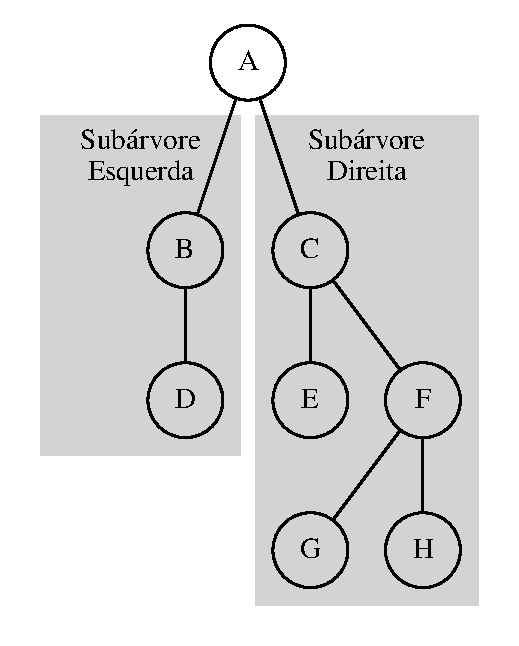
\includegraphics[height=0.5\paperheight]{imagens/arvore_binaria01-v2.eps}
\end{figure}
\end{itemize}
\end{frame}

%-------------------------------------------------------
\begin{frame}[fragile]\frametitle{Árvore Binária}
\begin{itemize}
	\item Se o grau de um nodo é 1, deve-se especificar se a sua subárvore é a da esquerda ou a da direita
\begin{figure}[h]
	\centering
	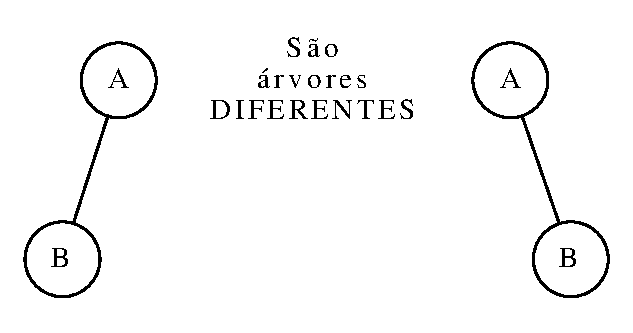
\includegraphics[height=0.35\paperheight]{imagens/arvores_binarias_diferentes.eps}
\end{figure}
\end{itemize}
\end{frame}

%-------------------------------------------------------
\begin{frame}[fragile]\frametitle{Árvore Binária Própria}
\begin{itemize}
	\item Uma árvore binária é \textbf{própria} se cada um de seus nodos internos tiver dois filhos
	\item Todos os nodos, com exceção dos nodos-folha, têm exatamente dois filhos
\begin{figure}[h]
	\centering
	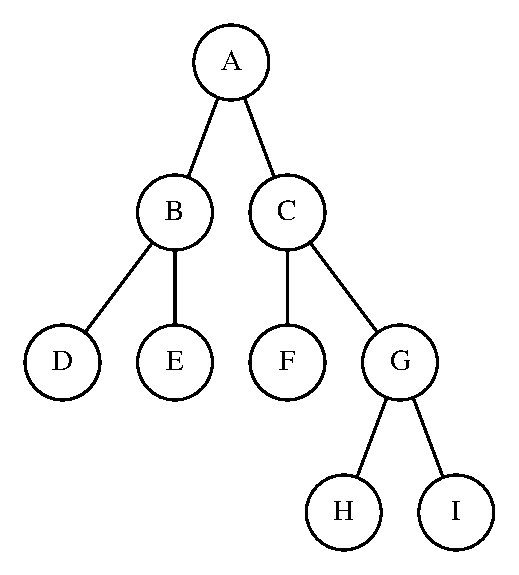
\includegraphics[height=0.5\paperheight]{imagens/arvore_binaria02.eps}
\end{figure}
\end{itemize}
\end{frame}

%-------------------------------------------------------
\begin{frame}[fragile]\frametitle{Árvores de Decisão}
\begin{itemize}
	\item Classe importante de árvores binárias
	\item Quando se quer representar as diferentes saídas que podem resultar a partir das respostas a um conjunto de perguntas do tipo sim ou não
	\item Cada nodo interno é associado com uma questão
\begin{figure}[h]
	\centering
	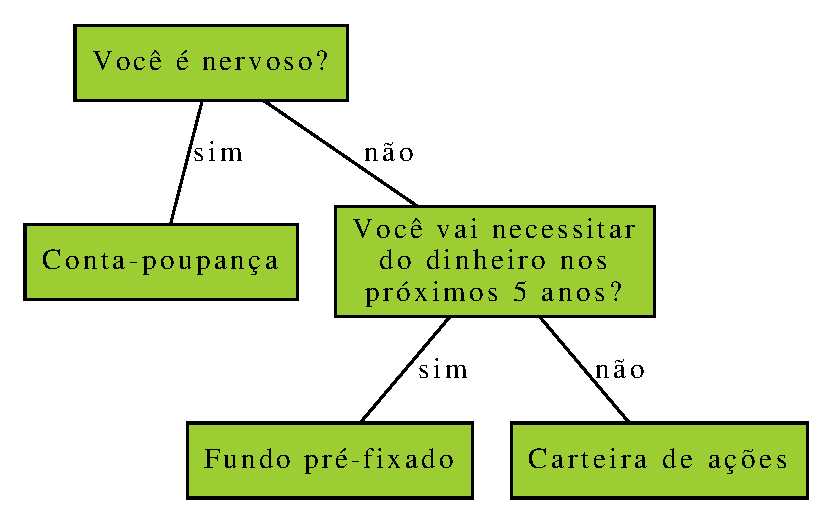
\includegraphics[height=0.5\paperheight]{imagens/arvore_de_decisao2.eps}
\end{figure}
\end{itemize}
\end{frame}

%-------------------------------------------------------
\begin{frame}\frametitle{Árvore Binária}
\begin{itemize}
	\item  Os nodos de uma árvore binária terão no mínimo:
	\begin{itemize}
		\item A informação
		\item Referência para o nodo da esquerda
		\item Referência para o nodo da direita
	\end{itemize}
	\item Também se pode usar referência para o nodo pai (o que facilita a ``navegação'')
	\item Árvores binárias são fáceis de implementar, pois cada nodo tem no máximo 2 filhos	
\end{itemize}
\end{frame}

%-------------------------------------------------------
\begin{frame}\frametitle{Árvore Binária}
\begin{columns}[T]
\begin{column}{0.2\linewidth}
%\vspace{-3mm}
\begin{figure}[h]
	\centering
	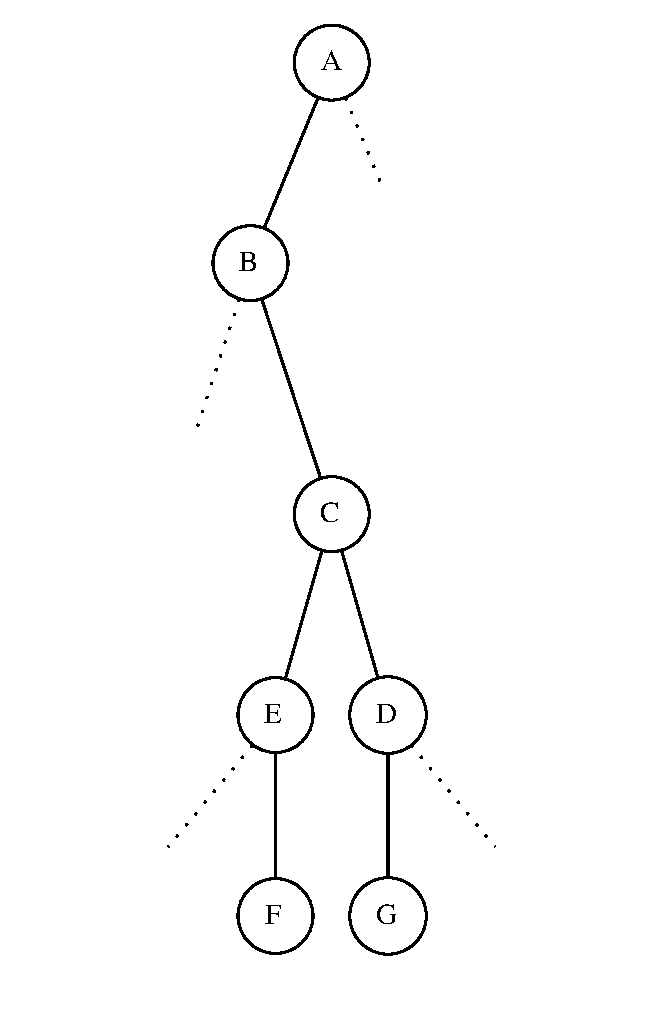
\includegraphics[height=0.70\paperheight]{imagens/arvore_binaria03.eps}
\end{figure}
\end{column}
\begin{column}{0.8\linewidth}
\vspace{-2mm}
\begin{figure}[h]
	\centering
	\textbf{\underline{SEM referência para o nodo-pai:}}\\	
	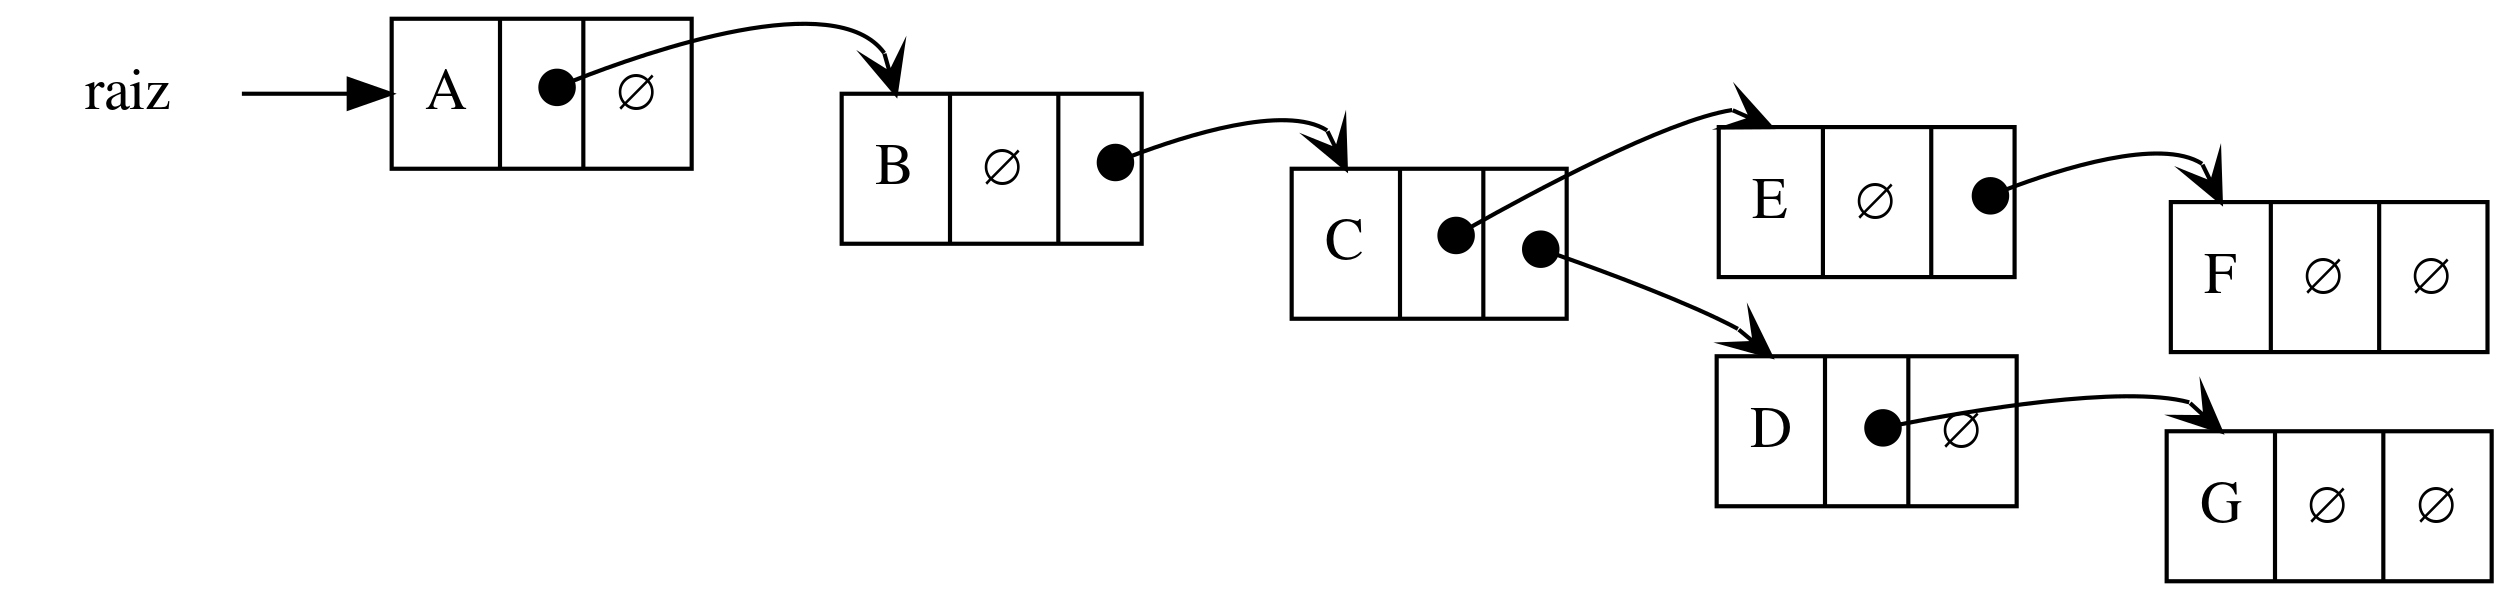
\includegraphics[height=0.3\paperheight]{imagens/arvore_binaria03-enc1.png}\\
	\textbf{\underline{COM referência para o nodo-pai:}}\\	
	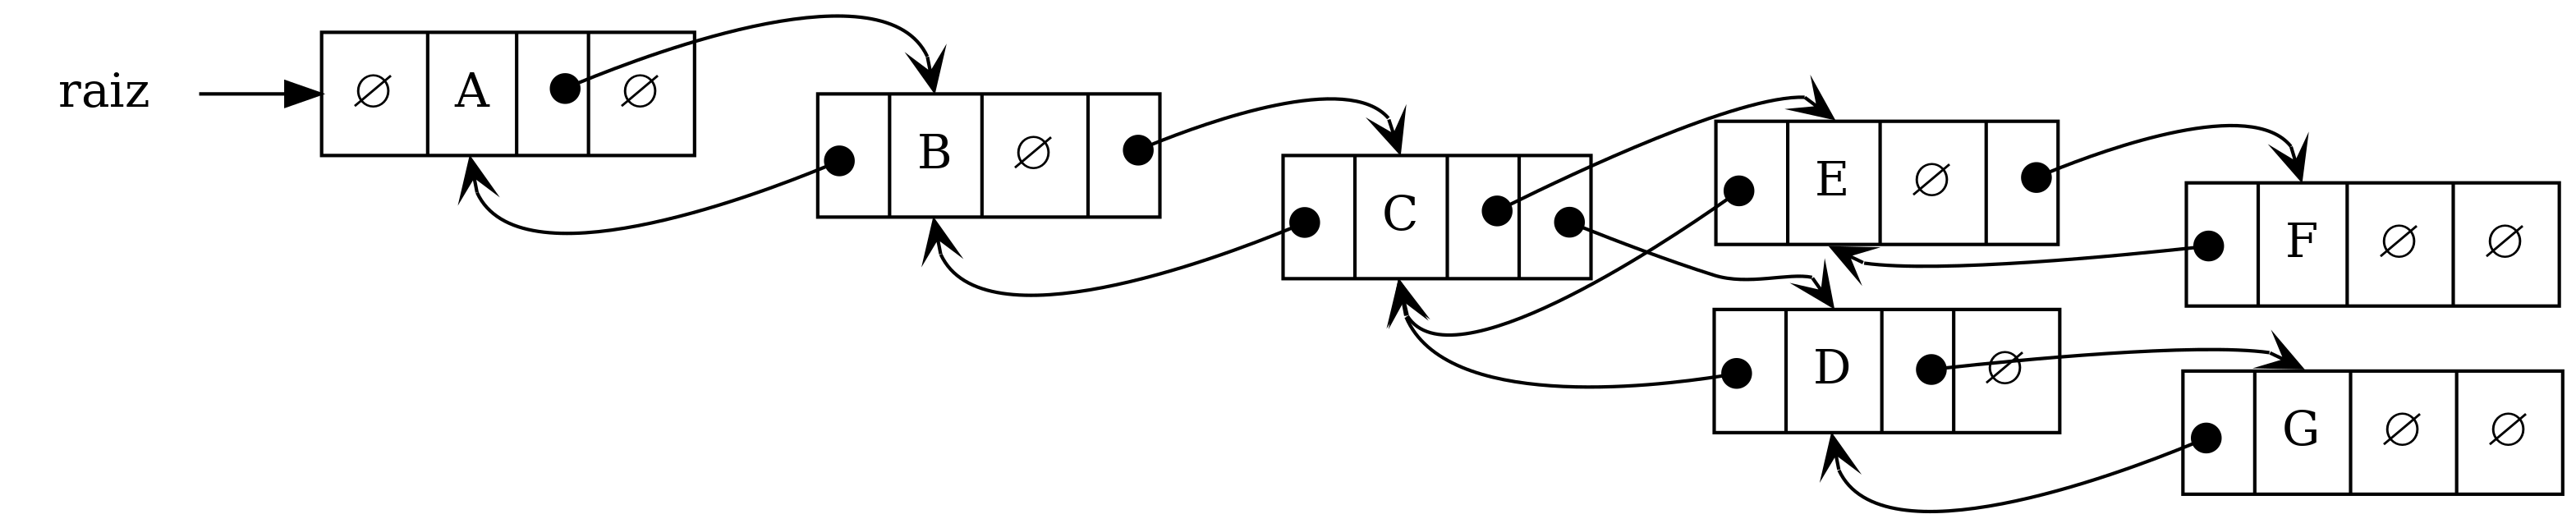
\includegraphics[height=0.27\paperheight]{imagens/arvore_binaria03-enc2.png}
\end{figure}
\end{column}
\end{columns}
\end{frame}

%-------------------------------------------------------
\begin{frame}\frametitle{Árvore Binária}
\begin{columns}[T]
\begin{column}{0.75\linewidth}
%\vspace{-3mm}
\begin{itemize}
	\item Uma árvore qualquer pode ser transformada em árvore binária\\
	\item Passos para a transformação:\\
	\begin{enumerate}
		\item Ligar os nodos irmãos
		\item Desligar a ligação do nodo pai com os filhos, exceto o primeiro filho
	\end{enumerate}
	\item Nodos de mesmo nível (irmãos) são encadeados à direita e nodos com nível maior (filhos) são encadeados à esquerda (iniciando pelo primeiro filho)
\end{itemize}
\vspace{-4mm}
\begin{figure}[h]
	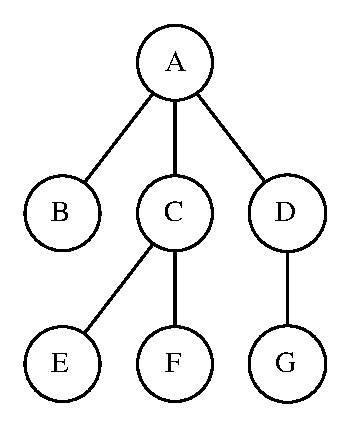
\includegraphics[height=0.3\paperheight]{imagens/arvore_b.eps} \hspace{25mm}
	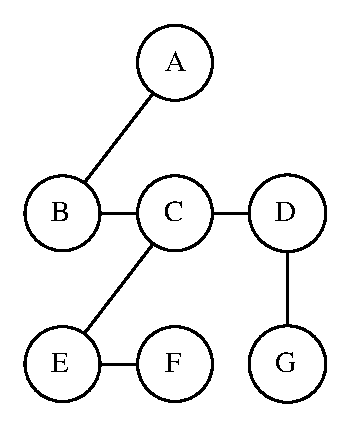
\includegraphics[height=0.3\paperheight]{imagens/arvore_b-v2.eps}
\end{figure}
\end{column}
\begin{column}{0.25\linewidth}
%\vspace{-2mm}
\begin{figure}[h]
	\centering
	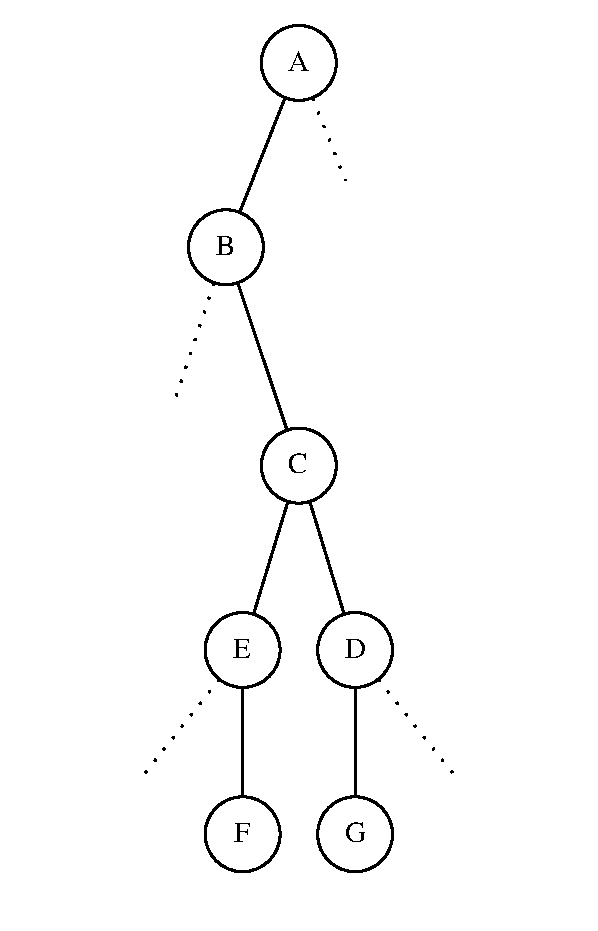
\includegraphics[height=0.7\paperheight]{imagens/arvore_b-v3.eps}
\end{figure}
\end{column}
\end{columns}
\end{frame}

%=======================================================
\section{Exercício}

%-------------------------------------------------------
\begin{frame}[fragile]\frametitle{Exercício 5}
\begin{columns}[T]
\begin{column}{0.75\linewidth}
\begin{enumerate}
        \setcounter{enumi}{4}
	\scriptsize
	\item O código apresentado nas duas páginas seguintes (\texttt{exercicio05.cpp}), define um nodo (\texttt{struct Node}) para uma árvore binária. Este nodo armazena: a informação (\texttt{info}, um único caractere), uma referência para o nodo pai (\texttt{parent}) e referências para as subárvores da esquerda (\texttt{left}) e direita (\texttt{right}). Além destas informações, o nodo contém um construtor e um destrutor. Juntamente com a definição do nodo são fornecidas funções para mostrar a árvore no formato GraphViz e uma função \texttt{main()}, que cria a árvore ao lado (usando o código fornecido) e realiza alguns testes com as funções que você deverá implementar.\\
	As funções que você deverá implementar são as seguintes:
	\begin{itemize}
		\tiny
		\item \texttt{int degree(Node *subtree)}: retorna o número de filhos (grau) de determinado nodo da árvore (parâmetro \texttt{subtree});
		\item \texttt{int depth(Node *subtree)}: retorna o nível de determinado nodo (parâmetro \texttt{subtree}) dentro da árvore (o que pode ser feito navegando pela árvore usando as referências para o nodos-pai, e contando o número de nodos até alcançar a raiz);
		\item \texttt{int height(Node *subtree)}: retorna o altura da árvore/subárvore a partir de um nodo específico (parâmetro \texttt{subtree}) -- deve ser implementado como uma função recursiva.
		\item \texttt{int size(Node *subtree)}: retorna o número de nodos que há na árvore a partir de determinado nodo (parâmetro \texttt{subtree}) -- deve ser implementado como uma função recursiva;
	\end{itemize}
Observação: os códigos usados neste exercício foram adaptados das soluções dos exercícios 3 e 4. As soluções, por outro lado, precisam ser desenvolvidas.
\end{enumerate}
\end{column}
\begin{column}{0.25\linewidth}
\begin{figure}[h]
	\centering
	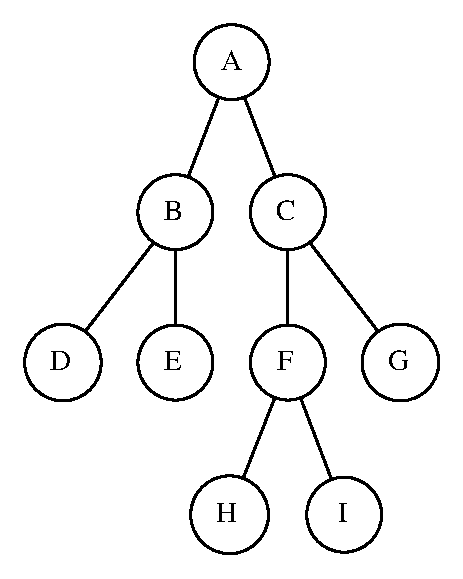
\includegraphics[height=0.4\paperheight]{imagens/exercicio05.eps}
\end{figure}
\end{column}
\end{columns}
\end{frame}

%-------------------------------------------------------
\begin{frame}[fragile]\frametitle{Exercício 5 (continuação)}
\fontsize{3pt}{5pt}\selectfont{
\lstinputlisting[firstline=1,lastline=36]{src/exercicio05.cpp}
}
\end{frame}

%-------------------------------------------------------
\begin{frame}[fragile]\frametitle{Exercício 5 (continuação)}
\fontsize{6pt}{6pt}\selectfont{
\lstinputlisting[firstline=38]{src/exercicio05.cpp}
}
\end{frame}

%=======================================================
\section{Observações}

%-------------------------------------------------------
\begin{frame}[fragile]\frametitle{Sobre a Implementação do Construtor do Exercício 5}
\begin{itemize}
	\item Observe o código que foi usado no construtor da \texttt{struct Node} do exercício 5:
\begin{lstlisting}[language=C++,basicstyle=\ttfamily\tiny]
Node(char i, Node *l = nullptr, Node *r = nullptr) {
  info = i;  left = l;  right = r;  parent = nullptr;
  if ( left != nullptr ) left->parent = this;
  if ( right != nullptr ) right->parent = this;
}
\end{lstlisting}
	\item Quando um nodo é criado, o construtor recebe as subárvores que serão inseridas como seus ``filhos''
	\item Como em cada nodo há uma referência para o nodo pai, este campo precisa ser atualizado nos nodos/subárvores filhos, o que é feito nas duas últimas linhas do construtor
	\item Para referenciar que os campos pai (\texttt{parent}) dos filhos (\texttt{left} e \texttt{right}) apontarão para o nodo que está sendo inicializado usa-se a autorreferência \texttt{\textbf{this}}
\end{itemize}
\end{frame}

%-------------------------------------------------------
\begin{frame}[fragile]\frametitle{Sobre a Solução do Exercício 5}
\begin{itemize}
	\item A solução do exercício 5 apresenta uma solução para o método \texttt{size()}, a princípio, mais fácil de entender:
\begin{lstlisting}[language=C++,basicstyle=\ttfamily\tiny]
int size(Node *subtree) {
  if (subtree == nullptr) return 0; // Somente pode ocorrer na primeira chamada,
  int res = 1;                      // ou seja, se a árvore estiver vazia
  if ( subtree->left != nullptr ) res += size(subtree->left);
  if ( subtree->right != nullptr ) res += size(subtree->right);
  return res;
}
\end{lstlisting}
	\item Veja uma solução alternativa e equivalente abaixo:
\begin{lstlisting}[language=C++,basicstyle=\ttfamily\tiny]
int size(Node *subtree) {
  if (subtree == nullptr) return 0;
  return 1 + size(subtree->left) + size(subtree->right);
}
\end{lstlisting}
	\item Analise as diferenças!
\end{itemize}
\end{frame}

%=======================================================
\section{Árvores Genéricas}

%-------------------------------------------------------
\begin{frame}\frametitle{Definição}
\begin{itemize}
	\item Formalmente uma árvore \textbf{T} é definida como um conjunto de \textbf{nodos}, que armazenam elementos em relacionamentos \textbf{pai-filho} com as seguintes propriedades:
	\begin{itemize}
		\item Se \textbf{T} não é vazia, ela tem um nodo especial chamado de \textbf{raiz} de \textbf{T} que não tem pai
		\item Cada nodo \textbf{v} de \textbf{T} diferente da raiz tem um único nodo \textbf{pai}, \textbf{w}; todo nodo com pai \textbf{w} é \textbf{filho} de \textbf{w}
	\end{itemize}
\end{itemize}
\end{frame}

%-------------------------------------------------------
\begin{frame}[fragile]\frametitle{Representações}
\begin{itemize}
	\item Textual
\begin{lstlisting}[basicstyle=\ttfamily\scriptsize]
T={A,{B,{D,{I},{J}},{E},{F}},{C,{G},{H,{K}}}}
\end{lstlisting}
\end{itemize}
\begin{columns}[T]
\begin{column}{0.5\linewidth}
%\vspace{-5mm}
\begin{itemize}
	\item GraphViz
	\lstinputlisting[basicstyle=\ttfamily\scriptsize]{imagens/arvore3.gv}
\end{itemize}
\end{column}
\begin{column}{0.5\linewidth}
\begin{itemize}
	\item Visual/Gráfica
\begin{figure}[h]
	\centering
	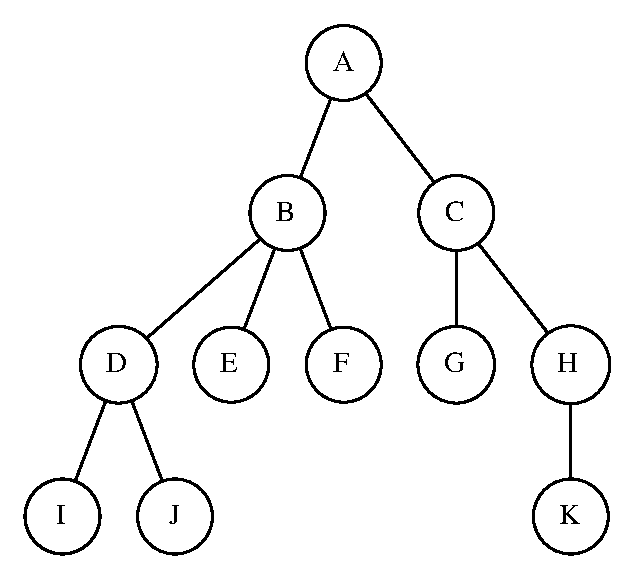
\includegraphics[height=0.4\paperheight]{imagens/arvore3.eps}
\end{figure}
\end{itemize}
\end{column}
\end{columns}
\end{frame}

%-------------------------------------------------------
\begin{frame}\frametitle{Operações}
\begin{itemize}
	\scriptsize
	\item Alocar nodos
	\item Desalocar nodos e seus descendentes
	\item Obter a informação de um nodo
	\item Obter a referência do nodo-pai de um nodo
	\item Inserir nodos ou subárvores como filhos de outro nodo
	\item Obter o grau (número de filhos) de um nodo
	\item Obter a referência para determinado nodo-filho de um nodo
	\item Remover determinado nodo-filho de um nodo
	\item Verificar se um nodo é raiz, interno ou externo
	\item Obter o nível de determinado nodo
	\item Obter o número de nodos a partir de determinado nodo da árvore
	\item Determinar a altura de uma árvore
	\item Verificar se determinada informação aparece a partir de um nodo
	\item Localizar o nodo que armazena determinada informação
	\item Percorrer a árvore
	\item Obter representações da árvore ou de subárvores em formatos específicos
	\item etc.
\end{itemize}
\end{frame}

%-------------------------------------------------------
\begin{frame}\frametitle{TAD para Árvores Genéricas}
\begin{itemize}
	\item A forma mais usual de implementação consiste no uso de \textbf{estruturas encadeadas} (alocação dinâmica)
	\item Cada nodo contém:
	\begin{itemize}
		\item A informação
		\item Uma referência para o nodo pai
		\item Uma lista de referências para os nodos filhos (subárvores)
	\end{itemize}
	\item Também é comum armazenar para uma árvore, o seu número total de nodos
\end{itemize}
\end{frame}

%-------------------------------------------------------
\begin{frame}[fragile]\frametitle{Lista de Referências para os Nodos Filhos}
\begin{itemize}
	\item Como um nodo pode ter número variável de filhos, é interessante trabalhar com uma lista dinamicamente expansível
	\item Para implemenar esta lista dinamicamente expansível é possível usar o \emph{container} \texttt{vector} da \emph{Standard Template Library} da linguagem C++
	\item Exemplo de uso de \texttt{vector}:
\begin{lstlisting}[language=C++,basicstyle=\ttfamily\tiny]
#include <vector>

// ...

vector<int> v;   // Cria um vetor de inteiros vazio
v.push_back(10); // Adiciona 10 no vetor -> v = { 10 }
v.push_back(20); // Adiciona 20 no vetor -> v = { 10, 20 }
v.push_back(30); // Adiciona 30 no vetor -> v = { 10, 20, 30 }
v.push_back(40); // Adiciona 40 no vetor -> v = { 10, 20, 30, 40 }
v.erase( v.begin() + 1 );  // Remove o elemento de índice 1 do vetor -> v = { 10, 30, 40 }
v.pop_back();              // Remove o último elemento do vetor -> v = { 10, 30 }
for (int i=0; i<v.size(); ++i) // mostra o vetor
    cout << v[i] << endl;      // v é usado como se fosse um arranjo
\end{lstlisting}
\end{itemize}
\end{frame}

%-------------------------------------------------------
\begin{frame}\frametitle{TAD para Árvores Genéricas}
\begin{itemize}
	\item É possível declarar um TAD para:
	\begin{itemize}
		\item A \textbf{estrutura de dados}, que terá uma classe interna para o nodo, determinando automaticamente onde cada informação será inserida (chamadas para acrescentar e remover algum dado NÃO especificam onde a informação será inserida; nodos e referências que formam a árvore permanecem encapsulados)
		\item O \textbf{nodo}, deixando o gerenciamento da árvore a cargo da própria aplicação (é necessário fornecer chamadas para acrescentar nodos-filho em determinado nodo, e também para remover nodos-filhos, etc.)
	\end{itemize}
\end{itemize}
\end{frame}

%-------------------------------------------------------
\begin{frame}\frametitle{Exemplo de TAD para uma Árvores de Inteiros}
\fontsize{3pt}{5pt}\selectfont{
\lstinputlisting{src/IntTree.hpp}
}
\end{frame}

%-------------------------------------------------------	
\begin{frame}[fragile]\frametitle{Exemplo de TAD para um Nodo de Árvore de Caracteres}
\fontsize{3pt}{5pt}\selectfont{
\lstinputlisting{src/exercicio06/NodeCharTree.hpp}
}
\end{frame}

%-------------------------------------------------------
\begin{frame}[fragile]\frametitle{Criando uma Árvore de Caracteres (Passo 1)}
\begin{columns}[T]
\begin{column}{0.5\linewidth}
\textbf{\underline{Código:}}
\begin{lstlisting}[language=C++,basicstyle=\ttfamily\tiny]
// Criação de nodos
NodeCharTree *b = new NodeCharTree('B');
NodeCharTree *a = new NodeCharTree('A');
NodeCharTree *d = new NodeCharTree('D');
NodeCharTree *f = new NodeCharTree('F');
NodeCharTree *c = new NodeCharTree('C');
NodeCharTree *e = new NodeCharTree('E');
\end{lstlisting}
~\\
\textbf{\underline{Memória:}}
{\tiny
\begin{verbatim}
b = ref1 --> |info='B'|parent=nullptr|childs={}|
a = ref2 --> |info='A'|parent=nullptr|childs={}|
d = ref3 --> |info='D'|parent=nullptr|childs={}|
f = ref4 --> |info='F'|parent=nullptr|childs={}|
c = ref5 --> |info='C'|parent=nullptr|childs={}|
e = ref6 --> |info='E'|parent=nullptr|childs={}|
\end{verbatim}
}
\end{column}
\begin{column}{0.5\linewidth}
\begin{figure}[h]
	\centering
	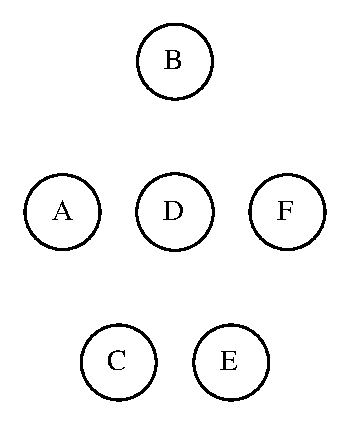
\includegraphics[height=0.4\paperheight]{imagens/arvore_c-passo1.eps}
\end{figure}
\end{column}
\end{columns}
\end{frame}

%-------------------------------------------------------
\begin{frame}[fragile]\frametitle{Criando uma Árvore de Caracteres (Passo 2)}
\begin{columns}[T]
\begin{column}{0.5\linewidth}
\textbf{\underline{Código:}}
\begin{lstlisting}[language=C++,basicstyle=\ttfamily\tiny]
// Adicionando os filhos de D
d->addSubtree( c );
d->addSubtree( e );
\end{lstlisting}
~\\
\textbf{\underline{Memória:}}
{\tiny
\begin{verbatim}
b = ref1 --> |info='B'|parent=nullptr|childs={}|
a = ref2 --> |info='A'|parent=nullptr|childs={}|
d = ref3 --> |info='D'|parent=nullptr|childs={ref5,ref6}|
f = ref4 --> |info='F'|parent=nullptr|childs={}|
c = ref5 --> |info='C'|parent=ref3   |childs={}|
e = ref6 --> |info='E'|parent=ref3   |childs={}|
\end{verbatim}
}
\end{column}
\begin{column}{0.5\linewidth}
\begin{figure}[h]
	\centering
	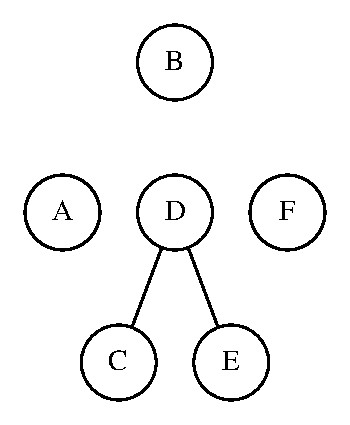
\includegraphics[height=0.4\paperheight]{imagens/arvore_c-passo2.eps}
\end{figure}
\end{column}
\end{columns}
\end{frame}

%-------------------------------------------------------
\begin{frame}[fragile]\frametitle{Criando uma Árvore de Caracteres (Passo Final)}
\begin{columns}[T]
\begin{column}{0.5\linewidth}
\textbf{\underline{Código:}}
\begin{lstlisting}[language=C++,basicstyle=\ttfamily\tiny]
// Adicionando os filhos de B
b->addSubtree( a );
b->addSubtree( d );
b->addSubtree( f );
\end{lstlisting}
~\\
\textbf{\underline{Memória:}}
{\tiny
\begin{verbatim}
b = ref1 --> |info='B'|parent=nullptr|childs={ref2,ref3,ref4}|
a = ref2 --> |info='A'|parent=ref1   |childs={}|
d = ref3 --> |info='D'|parent=ref1   |childs={ref5,ref6}|
f = ref4 --> |info='F'|parent=ref1   |childs={}|
c = ref5 --> |info='C'|parent=ref3   |childs={}|
e = ref6 --> |info='E'|parent=ref3   |childs={}|
\end{verbatim}
}
\end{column}
\begin{column}{0.5\linewidth}
\begin{figure}[h]
	\centering
	\includegraphics[height=0.4\paperheight]{imagens/arvore_c.eps}
\end{figure}
\end{column}
\end{columns}
\end{frame}

%=======================================================
\section{Exercício}

%-------------------------------------------------------
\begin{frame}[fragile]\frametitle{Exercício 6}
\begin{enumerate}
        \setcounter{enumi}{5}
	\small
	\item Nas páginas a seguir, há 3 arquivos, respectivamente, com: a definição da classe \texttt{NodeCharTree} (arquivo \texttt{exercicio06/NodeCharTree.hpp} e duas aplicações para testar a implementação dessa classe (arquivos \texttt{exercicio06/app1.cpp} e \texttt{exercicio06/app2.cpp}. Ambas as aplicações criam a árvore abaixo e testam a implementação da classe. Você encontra estes arquivos, juntamente com resultados esperados para a sua execução, no arquivo \texttt{src.zip} (disponível no Moodle da disciplina). A descrição do que cada método faz encontra-se nos comentários da definição da classe. \textbf{Implemente os métodos da classe no arquivo \texttt{exercicio06/NodeCharTree.cpp}}.
\begin{figure}[h]
	\centering
	\includegraphics[height=0.4\paperheight]{imagens/arvore3.eps}
\end{figure}
\end{enumerate}
\end{frame}

%-------------------------------------------------------
\begin{frame}[fragile]\frametitle{Exercício 6: \texttt{exercicio06/NodeCharTree.hpp}}
\fontsize{3pt}{5pt}\selectfont{
\lstinputlisting{src/exercicio06/NodeCharTree.hpp}
}
\end{frame}

%-------------------------------------------------------
\begin{frame}[fragile]\frametitle{Exercício 6: \texttt{exercicio06/app1.cpp}}
\fontsize{6pt}{6pt}\selectfont{
\lstinputlisting{src/exercicio06/app1.cpp}
}
\end{frame}

%-------------------------------------------------------
\begin{frame}[fragile]\frametitle{Exercício 6: \texttt{exercicio06/app2.cpp}}
\fontsize{3pt}{5pt}\selectfont{
\lstinputlisting{src/exercicio06/app2.cpp}
}
\end{frame}

%=======================================================
\section{Caminhamento em Árvores Genéricas}

%-------------------------------------------------------
\begin{frame}\frametitle{Caminhamento}
\begin{itemize}
	\item Caminhamento é a forma como vamos percorrer as árvores, ou seja, a ordem em que vamos visitar seus nodos
	\item Existem vários tipos de caminhamento que permitem varrer a árvore de forma sistemática visitando cada nodo uma única vez
	\item Para uma árvore genérica é comum o uso de três formas de caminhamento: \textbf{pré-ordem}, \textbf{pós-ordem} e \textbf{em largura}
\end{itemize}
\end{frame}

%-------------------------------------------------------
\begin{frame}\frametitle{Pré-ordem (\emph{pre-order})}
\begin{itemize}
	\item Do inglês \emph{pre-order traversal}
	\item O nodo é visitado antes de seus descendentes
	\item É definido recursivamente como:
	\begin{itemize}
		\item Visite o nodo
		\item Realize um percurso em pré-ordem para cada uma das subárvores do nodo
	\end{itemize}
	\item Exemplo de aplicação:
	\begin{itemize}
		\item Impressão de um documento estruturado em capítulos
	\end{itemize}
\end{itemize}
\end{frame}

%-------------------------------------------------------
\begin{frame}\frametitle{Pré-ordem (\emph{pre-order})}
\begin{columns}[T]
\begin{column}{0.7\linewidth}
\begin{figure}[h]
	\centering
	\includegraphics[height=0.5\paperheight]{imagens/arvore_d.eps}
\end{figure}
\end{column}
\begin{column}{0.3\linewidth}
\pause
\begin{enumerate}
	\item A
	\item B
	\item E
	\item F
	\item C
	\item G
	\item H
	\item I
	\item D
\end{enumerate}
\end{column}
\end{columns}
\end{frame}

%-------------------------------------------------------
\begin{frame}\frametitle{Pós-ordem (\emph{post-order})}
\begin{itemize}
	\item Do inglês \emph{post-order traversal}
	\item O nodo é visitado depois de seus descentes
	\item É definido recursivamente como:
	\begin{itemize}
		\item Realize um percurso em pós-ordem para cada uma das subárvores do nodo
		\item Visite o nodo
	\end{itemize}
	\item Exemplos de aplicação:
	\begin{itemize}
		\item Calcular o total de espaço em disco ocupado por arquivos em um sistema de diretórios
	\end{itemize}
\end{itemize}
\end{frame}

%-------------------------------------------------------
\begin{frame}\frametitle{Pós-ordem (\emph{post-order})}
\begin{columns}[T]
\begin{column}{0.7\linewidth}
\begin{figure}[h]
	\centering
	\includegraphics[height=0.5\paperheight]{imagens/arvore_d.eps}
\end{figure}
\end{column}
\begin{column}{0.3\linewidth}
\pause
\begin{enumerate}
	\item E
	\item F
	\item B
	\item G
	\item H
	\item I
	\item C
	\item D
	\item A
\end{enumerate}
\end{column}
\end{columns}
\end{frame}

%-------------------------------------------------------
\begin{frame}\frametitle{Em Largura (\emph{level-order})}
\begin{itemize}
	\item Visita os nodos na ordem dos níveis da árvore, da esquerda para a direita
	\begin{itemize}
		\item Visite os nodos de nível 0
		\item Visite os nodos de nível 1
		\item ...
	\end{itemize}
	\item Algoritmo não-recursivo:
	\begin{itemize}
		\item Inserir nodo raiz em uma fila
		\item Repetir até que a fila esteja vazia
		\begin{itemize}
			\item Remover o nodo da fila	
			\item Visitar o nodo atual
			\item Inserir na fila, em ordem, cada subárvore não vazia do nodo atual
		\end{itemize}
	\end{itemize}
\end{itemize}
\end{frame}

%-------------------------------------------------------
\begin{frame}\frametitle{Em Largura (\emph{level-order})}
\begin{columns}[T]
\begin{column}{0.7\linewidth}
\begin{figure}[h]
	\centering
	\includegraphics[height=0.5\paperheight]{imagens/arvore_d.eps}
\end{figure}
\end{column}
\begin{column}{0.3\linewidth}
\pause
\begin{enumerate}
	\item A
	\item B
	\item C
	\item D
	\item E
	\item F
	\item G
	\item H
	\item I
\end{enumerate}
\end{column}
\end{columns}
\end{frame}

%=======================================================
\section{Observação}

%-------------------------------------------------------
\begin{frame}[fragile]\frametitle{\emph{Templates} em C++}
\begin{itemize}
	\small
	\item Até aqui foram implementadas \textbf{estruturas de dados} diferentes para armazenar \textbf{diferentes tipos de informação} (\texttt{int}, \texttt{char}, \texttt{string}, etc.), o que acaba gerando uma grande quantidade de \textbf{código repetido} ou no mínimo parecido
	\item É possível em C++, criar um \emph{template} para determinada estrutura de dados, de forma que a mesma implementação possa ser aproveitada para diferentes tipos
	\item Assim, em vez de uma classe \texttt{NodeCharTree}, teríamos a seguinte classe genérica:
\begin{lstlisting}[language=C++,basicstyle=\ttfamily\tiny]
template <typename T>
class NodeTree {
private:
  T info;
  NodeTree *parent;
  vector<NodeTree *> childs;
  // ...
\end{lstlisting}
	\item Um nodo poderia então ser criado usando-se, por exemplo:
\begin{lstlisting}[language=C++,basicstyle=\ttfamily\tiny]
  NodeTree<char> *a1 = new NodeTree<char>('A');
  NodeTree<string> *a2 = new NodeTree<string>("raiz");
\end{lstlisting}
	\item O material da disciplina de Programação Orientada a Objetos contém maiores detalhes
\end{itemize}
\end{frame}
%=======================================================
\section{Exercícios}

%-------------------------------------------------------
\begin{frame}[fragile]\frametitle{Exercício 7}
\begin{enumerate}
	\setcounter{enumi}{6}
	\item Para as árvores a seguir, mostrar a ordem que os elementos serão apresentados para cada caminhamento (pré-ordem, pós-ordem e em largura).

\begin{tabular}{p{0.4\textwidth}p{0.5\textwidth}}
a) & b)\\
\includegraphics[height=0.5\paperheight]{imagens/expressao_aritmetica.eps} & \includegraphics[height=0.55\paperheight]{imagens/arvore_e.eps}\\
\end{tabular}
\end{enumerate}
\end{frame}

%-------------------------------------------------------
\begin{frame}[fragile]\frametitle{Exercício 8}
\begin{enumerate}
	\setcounter{enumi}{7}
	\footnotesize
	\item Considerando a classe \texttt{NodeCharTree} (resposta do Exercício 6), crie para esta classe três novos métodos que implementam os três tipos de caminhamento vistos até aqui (pré-ordem, pós-ordem e em largura). Estes caminhamentos devem ser implementados em métodos que geram uma cadeia de caracteres com o conteúdo dos nodos, na respectiva ordem do caminhamento, cada nodo em uma linha separada. Em \texttt{NodeCharTree.hpp}, acrescente:
\begin{lstlisting}[language=C++,basicstyle=\ttfamily\tiny]
string preorder() const;   // Gera uma cadeia de caracteres (um nodo por linha) em pré-ordem
string postorder() const;  // Gera uma cadeia de caracteres (um nodo por linha) em pós-ordem
string levelorder() const; // Gera uma cadeia de caracteres (um nodo por linha) em largura
\end{lstlisting}
Implemente estes métodos em \texttt{NodeCharTree.cpp} e use o programa da próxima página para testar a sua implementação. Este programa cria a árvore abaixo e mostra, para esta árvore, os resultados dos métodos a serem implementados.
\begin{figure}[h]
	\centering
	\includegraphics[height=0.3\paperheight]{imagens/arvore_d.eps}
\end{figure}
\end{enumerate}
\end{frame}

%-------------------------------------------------------
\begin{frame}[fragile]\frametitle{Exercício 8: \texttt{exercicio08/app.cpp}}
\lstinputlisting[basicstyle=\ttfamily\tiny]{src/exercicio08/app.cpp}
\end{frame}

%-------------------------------------------------------
\begin{frame}[fragile]\frametitle{Exercício 9 (DESAFIO)}
\begin{enumerate}
	\setcounter{enumi}{8}
	\footnotesize
	\item Considerando a classe \texttt{NodeCharTree} (resposta do Exercício 8), crie uma versão genérica desta classe usando \emph{templates}. A declaração da classe deve ser colocada em um arquivo chamado \texttt{NodeTree.hpp}. A \textbf{parte inicial} do arquivo \texttt{NodeTree.hpp} e a versão do arquivo \texttt{app.cpp} que usa esta classe genérica encontram-se nas páginas a seguir.\\
	Lembre-se de que a implementação dos métodos da classe genérica \texttt{NodeTree} deve ser colocada no próprio arquivo  \texttt{NodeTree.hpp}.\\
	Por sua vez, o arquivo \texttt{app.cpp} cria a árvore abaixo e mostra os caminhamentos em pré-ordem, pós-ordem e em largura para esta árvore.
\begin{figure}[h]
	\centering
	\includegraphics[height=0.3\paperheight]{imagens/arvore_d.eps}
\end{figure}
\end{enumerate}
\end{frame}

%-------------------------------------------------------
\begin{frame}[fragile]\frametitle{Exercício 9 (DESAFIO): \texttt{exercicio09/NodeTree.hpp} (início)}
\fontsize{3pt}{5pt}\selectfont{
\lstinputlisting[firstline=1,lastline=38]{src/exercicio09/NodeTree.hpp}
}
\end{frame}

%-------------------------------------------------------
\begin{frame}[fragile]\frametitle{Exercício 9 (DESAFIO): \texttt{exercicio09/app.cpp}}
\lstinputlisting[basicstyle=\ttfamily\tiny]{src/exercicio09/app.cpp}
\end{frame}

%-------------------------------------------------------
\begin{frame}[fragile]\frametitle{Exercício 10 (DESAFIO)}
\begin{columns}
\begin{column}{0.6\linewidth}
\begin{enumerate}
	\scriptsize
	\setcounter{enumi}{9}
	\item Comandos como o \texttt{pstree} do Unix, na versão para GNU/Linux, por exemplo, conseguem imprimir a árvore hierárquica de processos (que é uma árvore genérica) de uma forma visualmente agradável, como mostrado na figura ao lado.\\
Implemente na classe \texttt{NodeCharTree} (resposta do Exercício 8) uma funcionalidade semelhante. Em \texttt{NodeCharTree.hpp}, acrescente:
\begin{lstlisting}[language=C++,basicstyle=\ttfamily\tiny]
string strTree() const;
\end{lstlisting}
Este método deve gerar, por exemplo, uma cadeia de caracteres equivalente à representação ao lado para a árvore abaixo.
\begin{figure}[h]
	\centering
	\includegraphics[height=0.25\paperheight]{imagens/arvore3.eps}
\end{figure}
\end{enumerate}
\end{column}
\begin{column}{0.4\linewidth}
\begin{figure}[h]
	\centering
	\includegraphics[height=0.4\paperheight]{imagens/pstree.png}
\end{figure}
\vspace{3mm}
\begin{figure}[h]
	\centering
	\includegraphics[height=0.15\paperheight]{imagens/strtree.png}
\end{figure}
\end{column}
\end{columns}
\end{frame}

%=======================================================
\section{Árvores Binárias}

%-------------------------------------------------------
\begin{frame}\frametitle{Árvores Binárias}
\begin{itemize}
	\item Uma árvore binária é uma árvore ordenada com as seguintes propriedades:
	\begin{itemize}
		\item Todos os nodos tem no máximo dois filhos
		\item Cada nodo filho é rotulado como sendo um \textbf{filho da esquerda} ou um \textbf{filho da direita}
		\item O filho da esquerda precede o filho da direita na ordenação dos filhos de um nodo
	\end{itemize}
	\item Subárvores:
	\begin{itemize}
		\item O filho da esquerda de um nodo interno \textbf{v} é chamado de \textbf{subárvore da esquerda}
		\item O filho da direita de um nodo interno \textbf{v} é chamado de \textbf{subárvore da direita}
	\end{itemize}
	\item Árvore binária própria (ou cheia)
	\begin{itemize}
		\item Cada nodo tem 0 ou 2 filhos
	\end{itemize}
	\item As estruturas de árvores binárias são muito utilizadas na computação
\end{itemize}
\end{frame}

%-------------------------------------------------------
\begin{frame}\frametitle{Exemplo: Árvore para uma Expressão Aritmética}
\begin{itemize}
	\item Nodos externos são associados com variáveis e constantes
	\item Nodos internos são associados com um operador
	\item Exemplo: \texttt{(((3+1)*3)/((9-5)+2))-(3*(7-4)+6)}
\end{itemize}
\begin{figure}[h]
	\centering
	\includegraphics[height=0.55\paperheight]{imagens/arvore_binaria09-expressao.eps}
\end{figure}
\end{frame}

%-------------------------------------------------------
\begin{frame}\frametitle{Exemplo: Árvore de Decisão}
\begin{itemize}
	\item Árvore de decisão que fornece recomendações para um investidor
\begin{figure}[h]
	\centering
	\includegraphics[height=0.65\paperheight]{imagens/arvore_de_decisao3.eps}
\end{figure}
\end{itemize}
\end{frame}

%-------------------------------------------------------
\begin{frame}\frametitle{TAD para Árvores Binárias}
\begin{itemize}
	\item Forma mais usual de implementação é usando estruturas encadeadas, sendo que cada nó contém:
	\begin{itemize}
		\item A informação
		\item Uma referência para o nodo pai
		\item Uma referência para a subárvore da esquerda
		\item Uma referência para a subárvore da direita
	\end{itemize}
	\item Também é comum armazenar para uma árvore, o seu número total de nodos
	\item Da mesma forma que com árvores genéricas, é possível criar uma TAD para árvores binárias para:
	\begin{itemize}
		\item A \textbf{estrutura de dados}, que terá uma classe interna para o nodo, determinando automaticamente onde cada informação será inserida
		\item O \textbf{nodo}, deixando o gerenciamento da árvore a cargo da própria aplicação
	\end{itemize}
\end{itemize}
\end{frame}

%-------------------------------------------------------
\begin{frame}\frametitle{TAD para Árvores Binárias}
\begin{itemize}
	\item Para manipular uma árvore implementada como um TAD (ou seja, TAD para a estrutura de dados), pode-se ter métodos para:
	\begin{itemize}
		\item Criar a árvore
		\item Inserir nodos na árvore
		\item Pesquisar nodos na árvore
		\item Excluir nodos da árvore
		\item Determinar a altura da árvore e o nível de um nodo
		\item Caminhar em uma árvore, visitando seus nodos
		\item ...
	\end{itemize}
	\item Neste caso, o TAD contém uma classe interna para os nodos e armazena uma referência para a raiz da árvore e o número de elementos já inseridos
\end{itemize}
\end{frame}

%-------------------------------------------------------
\begin{frame}\frametitle{Exemplo de TAD para uma Árvores Binária de Inteiros}
\fontsize{3pt}{5pt}\selectfont{
\lstinputlisting[firstline=7,lastline=41]{src/IntBTree.hpp}
}
\end{frame}

%-------------------------------------------------------
\begin{frame}[fragile]\frametitle{Exemplo de TAD para um Nodo de Árvore Binária Genérica}
\fontsize{3pt}{5pt}\selectfont{
\lstinputlisting[firstline=11,lastline=42]{src/exercicio13/NodeBT.hpp}
}
\end{frame}

%-------------------------------------------------------
\begin{frame}\frametitle{Caminhamento}
\begin{itemize}
	\item Existem essencialmente duas formas diferentes de caminhamento:
	\begin{itemize}
		\item Percurso em profundidade
		\begin{itemize}
			\item Percurso pré-fixado ou em pré-ordem
			\item Percurso pós-fixado ou em pós-ordem
			\item Percurso central ou em ordem central
		\end{itemize}
		\item Percurso em largura
	\end{itemize}
\end{itemize}
\end{frame}

%-------------------------------------------------------
\begin{frame}\frametitle{Caminhamento Pré-fixado}
\begin{itemize}
	\item O nodo é visitado antes de seus descendentes
	\item Segue a ordem:
	\begin{itemize}
		\item Visita Raiz
		\item Percorre subárvore da esquerda
		\item Percorre subárvore da direita
	\end{itemize}
\end{itemize}
\begin{columns}[T]
\begin{column}{0.7\linewidth}
\begin{figure}[h]
	\centering
	\includegraphics[height=0.4\paperheight]{imagens/arvore_binaria08.eps}
\end{figure}
\end{column}
\begin{column}{0.3\linewidth}
\pause
\begin{enumerate}
	\item A
	\item B
	\item D
	\item E
	\item C
	\item F
	\item G
\end{enumerate}
\end{column}
\end{columns}
\end{frame}

%-------------------------------------------------------
\begin{frame}\frametitle{Caminhamento Pós-fixado}
\begin{itemize}
	\item O nodo é visitado depois de seus descentes
	\item Segue a ordem:
	\begin{itemize}
		\item Percorre subárvore da esquerda
		\item Percorre subárvore da direita
		\item Visita Raiz
	\end{itemize}
\end{itemize}
\begin{columns}[T]
\begin{column}{0.7\linewidth}
\begin{figure}[h]
	\centering
	\includegraphics[height=0.4\paperheight]{imagens/arvore_binaria08.eps}
\end{figure}
\end{column}
\begin{column}{0.3\linewidth}
\pause
\begin{enumerate}
	\item D
	\item E
	\item B
	\item F
	\item G
	\item C
	\item A
\end{enumerate}
\end{column}
\end{columns}
\end{frame}

%-------------------------------------------------------
\begin{frame}\frametitle{Caminhamento Central (\emph{In-order})	}
\begin{itemize}
	\item Segue a ordem:
	\begin{itemize}
		\item Percorre subárvore da esquerda
		\item Visita Raiz
		\item Percorre subárvore da direita
	\end{itemize}
\end{itemize}
\begin{columns}[T]
\begin{column}{0.7\linewidth}
\begin{figure}[h]
	\centering
	\includegraphics[height=0.4\paperheight]{imagens/arvore_binaria08.eps}
\end{figure}
\end{column}
\begin{column}{0.3\linewidth}
\pause
\begin{enumerate}
	\item D
	\item B
	\item E
	\item A
	\item C
	\item F
	\item G
\end{enumerate}
\end{column}
\end{columns}
\end{frame}

%-------------------------------------------------------
\begin{frame}\frametitle{Caminhamento em Largura}
\begin{itemize}
	\item Visita os nodos na ordem dos níveis da árvore, da esquerda para a direita
	\begin{itemize}
		\item Visite os nodos de nível 0
		\item Visite os nodos de nível 1
		\item ...
	\end{itemize}
\end{itemize}
\begin{columns}[T]
\begin{column}{0.7\linewidth}
\begin{figure}[h]
	\centering
	\includegraphics[height=0.4\paperheight]{imagens/arvore_binaria08.eps}
\end{figure}
\end{column}
\begin{column}{0.3\linewidth}
\pause
\begin{enumerate}
	\item A
	\item B
	\item C
	\item D
	\item E
	\item F
	\item G
\end{enumerate}
\end{column}
\end{columns}
\end{frame}

%=======================================================
\section{Exercícios}

%-------------------------------------------------------
\begin{frame}[fragile]\frametitle{Exercícios 11 e 12}
\begin{enumerate}
	\setcounter{enumi}{10}
	\item Monte a árvore binária para a seguinte seguinte expressão aritmética:
\texttt{(A+B)-(C*(D-E)+(F/G))}.
	\item Apresente os caminhamentos pré-fixado, pós-fixado, central e em largura para as seguintes árvores binárias. \begin{tabular}{llll}%p{0.10\textwidth}p{0.15\textwidth}p{0.25\textwidth}p{0.25\textwidth}}
a) & b) & c) & d)\\
\includegraphics[height=0.5\paperheight]{imagens/arvore_binaria04.eps} &
\includegraphics[height=0.5\paperheight]{imagens/arvore_binaria05.eps} &
\includegraphics[height=0.5\paperheight]{imagens/arvore_binaria06.eps} &
\includegraphics[height=0.5\paperheight]{imagens/arvore_binaria07.eps} \\
\end{tabular}
\end{enumerate}
\end{frame}

%-------------------------------------------------------
\begin{frame}[fragile]\frametitle{Exercício 13}
\begin{columns}[T]
\begin{column}{0.75\linewidth}
%\vspace{-3mm}
\begin{enumerate}
	\setcounter{enumi}{12}
	\small
	\item Nas páginas a seguir, há a definição de uma classe genérica para gerenciamento dos nodos de uma árvore binária (\texttt{NodeBT}) -- cujos métodos devem ser implementados -- e uma aplicação para testar a implementação dessa classe (arquivo \texttt{exercicio13/app.cpp}). A aplicação cria a árvore ao lado e testa a implementação da classe sobre essa árvore. Você encontra este arquivo, juntamente com o resultado esperado para a sua execução, no arquivo \texttt{src.zip} (disponível no Moodle da disciplina). A descrição do que cada método faz encontra-se nos comentários da definição da classe. Por se tratar de um \emph{template}, lembre-se de colocar a definição da classe em um arquivo chamado \texttt{NodeBT.hpp} e de \textbf{implementar os métodos da classe nesse mesmo arquivo}.
\end{enumerate}
\end{column}
\begin{column}{0.25\linewidth}
\vspace{-3mm}
\begin{figure}[h]
	\centering
	\includegraphics[height=0.7\paperheight]{imagens/arvore_binaria05.eps}
\end{figure}
\end{column}
\end{columns}
\end{frame}

%-------------------------------------------------------
\begin{frame}[fragile]\frametitle{Trecho do arquivo \texttt{NodeBT.hpp}}
\fontsize{3pt}{5pt}\selectfont{
\lstinputlisting[firstline=11,lastline=42]{src/exercicio13/NodeBT.hpp}
}
\end{frame}

%-------------------------------------------------------
\begin{frame}[fragile]\frametitle{Exercício 13: \texttt{exercicio13/app.cpp}}
\fontsize{3pt}{5pt}\selectfont{
\lstinputlisting{src/exercicio13/app.cpp}
}
\end{frame}

%=======================================================
\section{Árvores Binárias de Pesquisa (ABP)}

%-------------------------------------------------------
\begin{frame}\frametitle{Introdução}
\begin{itemize}
	\item Árvores ``comuns'' não possuem restrição com relação às posições relativas de seus nodos
	\item Um item pode aparecer em qualquer posição da árvore
	\item Algoritmos de busca são ineficientes
	\begin{itemize}
		\item Pode ser necessário percorrer todos os nodos da árvore.
		\item $O(n)$
	\end{itemize}
\end{itemize}
\end{frame}

%-------------------------------------------------------
\begin{frame}\frametitle{Árvores Binárias de Pesquisa (ABP)}
\begin{itemize}
	\item Classe especial de árvores de busca
	\item Suportam operações eficientes de busca, inserção e remoção
	\begin{itemize}
		\item $O(\log{n})$, se balanceada
	\end{itemize}
	\item Apresentam restrições quanto à posição relativa dos nodos
	\begin{itemize}
		\item Possuem uma relação de ordem total entre os elementos armazenados (os elementos são usualmente chamados de ``chaves'')
	\end{itemize}
\end{itemize}
\end{frame}

%-------------------------------------------------------
\begin{frame}\frametitle{Árvores Binárias de Pesquisa (ABP)}
\begin{itemize}
	\item Seja $S$ um conjunto cujos elementos possuem uma relação de ordem (exemplo: conjunto de inteiros, lista de nomes, etc.)
	\item Uma árvore binária de pesquisa para $S$ é uma árvore binária $T$ tal que
	\begin{itemize}
		\item Cada nodo interno $v$ de $T$ armazena um elemento de $S$ denotado $x(v)$
		\item Para cada nodo interno $v$ de $T$, os elementos armazenados na subárvore esquerda de $v$ são menores ou iguais a $x(v)$, e os elementos armazenados na subárvore direita de $v$ são maiores ou iguais a $x(v)$
	\end{itemize}
\end{itemize}
\end{frame}

%-------------------------------------------------------
\begin{frame}\frametitle{Árvores Binárias de Pesquisa (ABP)}
\begin{itemize}
	\item Quando a árvore é montada
	\begin{itemize}
		\item Todos os elementos da subárvore esquerda são menores do que o elemento da raiz
		\item Todos os elementos da subárvore direita são maiores do que o elemento da raiz
	\end{itemize}
	\item Exemplo:
\begin{figure}[h]
	\centering
	\includegraphics[height=0.3\paperheight]{imagens/abp01.png}
\end{figure}
	\item Quando implementada, todos os métodos respeitam e fazem uso dessa ordenação
\end{itemize}
\end{frame}

%-------------------------------------------------------
\begin{frame}\frametitle{TAD para Árvores Binárias de Pesquisa (ABP)}
\begin{itemize}
	\item A ABP é implementada usando o nodo para árvore binária (\texttt{NodeBT})
	\begin{itemize}
		\item A forma mais usual de implementação é através de estruturas encadeadas	
		\item Cada nodo contém a informação e referências para nodo-pai, subárvore da esquerda e subárvore da direita
	\end{itemize}
	\item Deve ser possível comparar os elementos de uma árvore
	\begin{itemize}
		\item Em C++, classes devem ter os operadores relacionais corretamente sobrecarregadoso
		\item Em Java, objetos devem implementar a interface \texttt{Comparable}
	\end{itemize}
	\item Vários métodos são necessários para manipular uma árvore binária de pesquisa
	\begin{itemize}
		\item Inserir um elemento na árvore
		\item Localizar um elemento na árvore
		\item Remover um elemento da árvore
		\item Caminhar em uma árvore, visitando seus nodos
		\item ...
	\end{itemize}
\end{itemize}
\end{frame}

%-------------------------------------------------------
\begin{frame}\frametitle{TAD Genérico para Árvores Binárias de Pesquisa (ABP)}
\begin{itemize}
	\scriptsize
	\item \texttt{bool isEmpty()}: retorna \texttt{true} se a árvore está vazia\\
	\item \texttt{int size()}: retorna o número de elementos armazenados na árvore\\
	\item \texttt{void clear()}: remove todos os elementos da árvore\\
	\item \texttt{T getRoot()}: retorna o elemento armazenado na raiz\\
	\item \texttt{void add(T \&e)}: insere o elemento \texttt{e} na árvore de forma ordenada\\
	\item \texttt{bool remove(T \&e)}: remove o elemento \texttt{e} e reestrutura a árvore se necessário\\
	\item \texttt{T getLeft(T \&e)}: retorna o filho à esquerda de \texttt{e}\\
	\item \texttt{T getRight(T \&e)}: retorna o filho à direita de \texttt{e}\\
	\item \texttt{T getParent(T \&e)}: retorna o pai do elemento \texttt{e}\\
	\item \texttt{int level(T \&e)}: retorna o nível do elemento \texttt{e} e -1 caso o elemento não esteja na árvore\\
	\item \texttt{int height()}: retorna a altura da árvore\\
	\item \texttt{bool contains(T \&e)}: retorna \texttt{true} se a árvore contém o elemento \texttt{e}\\
	\item \texttt{bool isInternal(T \&e)}: retorna \texttt{true} se o elemento está armazenado em um nodo interno\\
	\item \texttt{bool isExternal(T \&e)}: retorna \texttt{true} se o elemento está armazenado em um nodo externo\\
	\item \texttt{vector<T> preorder()}: retorna um vetor com todos os elementos da árvore na ordem pré-fixada\\
	\item \texttt{vector<T> inorder()}: retorna um vetor com todos os elementos da árvore na ordem central\\
	\item \texttt{vector<T> postorder()}: retorna um vetor com todos os elementos da árvore na ordem pos-fixada\\
	\item \texttt{vector<T> levelorder()}: retorna uma lista com todos os elementos da árvore com um caminhamento em largura\\
\end{itemize}
\end{frame}

%-------------------------------------------------------
\begin{frame}\frametitle{Inserção em Árvores Binárias de Pesquisa (ABP)}
\begin{itemize}
	\item Se a árvore estiver vazia, então o elemento é a raiz
	\item Senão
	\begin{itemize}
		\item Se for menor, inserir na subárvore esquerda
		\item Se for maior ou igual, inserir na subárvore direita
	\end{itemize}
	\item Repetir este processo \textbf{recursivamente} até que chegue a uma subárvore vazia
	\item Neste ponto o novo valor é incluído
	\item Exemplo: \texttt{abp.add(5);}
\begin{figure}[h]
	\centering
	\includegraphics[height=0.3\paperheight]{imagens/abp-insercao.png}
\end{figure}
\end{itemize}
\end{frame}

%-------------------------------------------------------
\begin{frame}\frametitle{Busca Recursiva em Árvores Binárias de Pesquisa (ABP)}
\begin{itemize}
	\item Comparar o valor a ser localizado com a raiz
	\begin{itemize}
		\item Se for igual, então encontrou
		\item Se for menor, procura na subárvore esquerda
		\item Se for maior, procura na subárvore direita
	\end{itemize}
	\item Repetir este processo até encontrar ou até chegar a uma subárvore vazia (não encontrou)
	\item Exemplo: \texttt{abp.contains(4);}
\begin{figure}[h]
	\centering
	\includegraphics[height=0.3\paperheight]{imagens/abp-busca.png}
\end{figure}
\end{itemize}
\end{frame}

%-------------------------------------------------------
\begin{frame}\frametitle{Remoção em Árvores Binárias de Pesquisa (ABP)}
\begin{itemize}
	\item Trata-se de uma operação mais complexa, pois após a remoção é necessário que a árvore permaneça satisfazendo o critério de ordenação dos dados\\
	\item Exemplo: \texttt{abp.remove(2);}\\
\begin{figure}[h]
	\centering
	\includegraphics[height=0.3\paperheight]{imagens/abp-remocao1.png}
\end{figure}
	\item Algoritmo\\
	\begin{itemize}
		\item Localizar o elemento a ser excluído, e, se ele estiver na árvore, guardar quem é o seu pai\\
		\item Verificar se o elemento: é um nodo folha, tem 1 filho ou tem 2 filhos\\
		\item Excluir o nodo e reestruturar a árvore\\
	\end{itemize}
\end{itemize}
\end{frame}

%-------------------------------------------------------
\begin{frame}\frametitle{Remoção em Árvores Binárias de Pesquisa (ABP)}
\begin{itemize}
	\item Item a ser removido está em uma folha: remover o nodo\\
	\item Item a ser removido tem apenas um filho: remover o nodo e o filho ocupa seu lugar\\
	\item Item a ser removido tem dois filhos: trocar por um nodo folha e depois remover a folha. Há duas possibilidades:\\
	\begin{itemize}
		\item Trocar pelo menor item da subárvore direita\\
		\item Trocar pelo maior item da subárvore esquerda\\
	\end{itemize}
	\item Exemplo: \texttt{abp.remove(3);}\\
\begin{figure}[h]
	\centering
	\includegraphics[height=0.3\paperheight]{imagens/abp-remocao2.png}
\end{figure}
\end{itemize}
\end{frame}

%-------------------------------------------------------
\begin{frame}\frametitle{ABP: Caminhamento}
\begin{itemize}
	\item Os caminhamentos são os mesmos que já foram visto para árvores bináras:
	\begin{itemize}
		\item Percurso em profundidade
		\begin{itemize}
			\item Percurso pré-fixado ou em pré-ordem
			\item Percurso pós-fixado ou em pós-ordem
			\item Percurso central ou em ordem central
		\end{itemize}
		\item Percurso em largura
	\end{itemize}
\end{itemize}
\end{frame}

%-------------------------------------------------------
\begin{frame}\frametitle{ABP: Caminhamento Pré-fixado}
\begin{itemize}
	\item O nodo é visitado antes de seus descendentes
	\item Segue a ordem:
	\begin{itemize}
		\item Visita Raiz
		\item Percorre subárvore da esquerda
		\item Percorre subárvore da direita
	\end{itemize}
\end{itemize}
\begin{columns}[T]
\begin{column}{0.7\linewidth}
\begin{figure}[h]
	\centering
	\includegraphics[height=0.3\paperheight]{imagens/abp02.png}
\end{figure}
\end{column}
\begin{column}{0.3\linewidth}
\pause
\begin{enumerate}
	\small
	\item 15
	\item 9
	\item 2
	\item 11
	\item 23
	\item 20
	\item 38
\end{enumerate}
\end{column}
\end{columns}
\end{frame}

%-------------------------------------------------------
\begin{frame}\frametitle{ABP: Caminhamento Pós-fixado}
\begin{itemize}
	\item O nodo é visitado depois de seus descentes
	\item Segue a ordem:
	\begin{itemize}
		\item Percorre subárvore da esquerda
		\item Percorre subárvore da direita
		\item Visita Raiz
	\end{itemize}
\end{itemize}
\begin{columns}[T]
\begin{column}{0.7\linewidth}
\begin{figure}[h]
	\centering
	\includegraphics[height=0.3\paperheight]{imagens/abp02.png}
\end{figure}
\end{column}
\begin{column}{0.3\linewidth}
\pause
\begin{enumerate}
	\small
	\item 2
	\item 11
	\item 9
	\item 20
	\item 38
	\item 23
	\item 15
\end{enumerate}
\end{column}
\end{columns}
\end{frame}

%-------------------------------------------------------
\begin{frame}\frametitle{ABP: Caminhamento Central (\emph{In-order})}
\begin{itemize}
	\item Segue a ordem:
	\begin{itemize}
		\item Percorre subárvore da esquerda
		\item Visita Raiz
		\item Percorre subárvore da direita
	\end{itemize}
\end{itemize}
\begin{columns}[T]
\begin{column}{0.7\linewidth}
\begin{figure}[h]
	\centering
	\includegraphics[height=0.3\paperheight]{imagens/abp02.png}
\end{figure}
\end{column}
\begin{column}{0.3\linewidth}
\pause
\begin{enumerate}
	\small
	\item 2
	\item 9
	\item 11
	\item 15
	\item 20
	\item 23
	\item 38
\end{enumerate}
\end{column}
\end{columns}
\end{frame}

%-------------------------------------------------------
\begin{frame}\frametitle{ABP: Caminhamento Central (\emph{In-order})}
\begin{columns}[T]
\begin{column}{0.6\linewidth}
\begin{itemize}
	\item Em uma ABP, o caminhamento central sempre fornece os dados classificados em ordem crescente
	\item Exemplo:
	\begin{itemize}
		\item Considerando: Jan=1, ..., Dez=12
		\item \textbf{Pré-Fixado:} Jul, Abr, Mar, Jan, Fev, Jun, Mai, Dez, Nov, Ago, Out, Set
		\item \textbf{Central:}    Jan, Fev, Mar, Abr, Mai, Jun, Jul, Ago, Set, Out, Nov, Dez
		\item \textbf{Pós-Fixado:} Fev, Jan, Mar, Mai, Jun, Abr, Set, Out, Ago, Nov, Dez, Jul
	\end{itemize}
\end{itemize}
\end{column}
\begin{column}{0.4\linewidth}
\vspace{-3mm}
\begin{figure}[h]
	\centering
	\includegraphics[height=0.7\paperheight]{imagens/abp-meses.png}
\end{figure}
\end{column}
\end{columns}
\end{frame}

%-------------------------------------------------------
\begin{frame}\frametitle{ABP: Caminhamento em Largura}
\begin{itemize}
	\item Visita os nodos na ordem dos níveis da árvore, da esquerda para a direita
	\begin{itemize}
		\item Visite os nodos de nível 0
		\item Visite os nodos de nível 1
		\item ...
	\end{itemize}
\end{itemize}
\begin{columns}[T]
\begin{column}{0.7\linewidth}
\begin{figure}[h]
	\centering
	\includegraphics[height=0.3\paperheight]{imagens/abp02.png}
\end{figure}
\end{column}
\begin{column}{0.3\linewidth}
\pause
\begin{enumerate}
	\small
	\item 15
	\item 9
	\item 23
	\item 2
	\item 11
	\item 20
	\item 38
\end{enumerate}
\end{column}
\end{columns}
\end{frame}

%=======================================================
\section{Exercícios}

%-------------------------------------------------------
\begin{frame}[fragile]\frametitle{Exercício 14}
\begin{enumerate}
	\setcounter{enumi}{13}
	\item Mostre como ficaria uma ABP de inteiros, se fossem incluídos os seguintes elementos (nesta ordem):\\8, 2, 10, 6, 5, 15, 7, 3, 20, 11.\\
Verifique a sua solução usando a seguinte página: \url{https://www.cs.usfca.edu/~galles/visualization/BST.html}
\end{enumerate}
\end{frame}

%-------------------------------------------------------
\begin{frame}[fragile]\frametitle{Exercício 15}
\begin{enumerate}
	\setcounter{enumi}{14}
	\item Usando a classe genéria para nodo de uma árvore binária, classe \texttt{NodeBT} (desenvolvida no Exercício 13), implemente uma classe, também genérica, chamada \texttt{BST} (de \emph{Binary Search Tree}) de forma que esta classe tenha como variável de instância a referência para o nodo raiz:
\begin{lstlisting}[language=C++,basicstyle=\ttfamily\tiny]
NodeBT<T> *root;
\end{lstlisting}
Na interface pública desta classe implemente os seguintes métodos:
	\begin{itemize}
		\item \texttt{BST()}: construtor que simplesmente inicializa \texttt{root} com \texttt{nullptr}
		\item \texttt{\~{}BST()}: destrutor que remove todos os nodos da árvore
		\item \texttt{string strGraphViz() const}: mostra a árvore no formato GraphViz
		\item \texttt{void add(const T \&e)}: adiciona o elemento \texttt{e} na posição correta da árvore
		\item \texttt{bool contains(const T \&e)}: verifica se a árvore contém o elemento \texttt{e}
	\end{itemize}
O programa da próxima página usa a classe genérica \texttt{ABP} para criar a mesma árvore do Exercício 14.
\end{enumerate}
\end{frame}

%-------------------------------------------------------
\begin{frame}[fragile]\frametitle{Exercício 15: \texttt{exercicio15/app.cpp}}
\lstinputlisting[basicstyle=\ttfamily\scriptsize]{src/exercicio15/app.cpp}
\end{frame}

%=======================================================
\section{ABPs Balanceadas}

%-------------------------------------------------------
\begin{frame}\frametitle{Árvores Binárias de Pesquisa (ABP)}
\begin{itemize}
	\item ABPs apresentam restrições quanto à posição relativa dos nodos
	\item Suportam operações eficientes de busca e inserção \textbf{se estiverem balanceadas}
	\begin{itemize}
		\item $O(n)$, se não estiver balanceada
		\item $O(\log{n})$, se estiver balanceada
	\end{itemize}
\end{itemize}
\vspace{-3mm}
\begin{columns}[T]
\begin{column}{0.45\linewidth}
\begin{figure}[h]
	\centering
	\textbf{\underline{Árvore não balanceada}}\\~\\
	\includegraphics[height=0.4\paperheight]{imagens/abp03.png}
\end{figure}
\end{column}
\begin{column}{0.10\linewidth}
~\\~\\X
\end{column}
\begin{column}{0.45\linewidth}
\begin{figure}[h]
	\centering
	\textbf{\underline{Árvore balanceada}}\\~\\
	\includegraphics[height=0.32\paperheight]{imagens/avl01.png}
\end{figure}
	\end{column}
\end{columns}
\end{frame}	

%-------------------------------------------------------
\begin{frame}\frametitle{ABP Balanceada -- Introdução}
\begin{itemize}
	\item Usar estruturas de dados e algoritmos \textbf{eficientes e simples de implementar} é importante
	\item Uma ABP balanceada apresenta melhor (desempenho) que uma ABP
	\begin{itemize}
		\item Muitas vezes, árvores balanceadas podem ter um desempenho muito superior do que listas encadeadas e matrizes
	\end{itemize}	
	\item Critério para determinar se uma árvore não vazia é balanceada:
	\begin{itemize}
		\item Depende do tipo de árvore
		\item Exemplos de ABPs balanceadas:
		\begin{itemize}
			\item Árvores AVL\\
				\url{https://www.cs.usfca.edu/~galles/visualization/AVLtree.html}
			\item Árvores rubro-negras\\
				\url{https://www.cs.usfca.edu/~galles/visualization/RedBlack.html}
			\item Árvores de Andersson\\
				\url{https://en.wikipedia.org/wiki/AA_tree}
			\item \emph{Splay Tree} (nódos são reposicionados de acordo com a frequência de acesso)\\
				\url{https://www.cs.usfca.edu/~galles/visualization/SplayTree.html}
			\end{itemize}
	\end{itemize}
\end{itemize}
\end{frame}

%-------------------------------------------------------
\begin{frame}\frametitle{Árvores AVL}
\begin{itemize}
	\item Nome referente aos autores: G. M. \underline{A}delson-\underline{V}elskii e E. M. \underline{L}andis
	\item Operações de busca, inserção e remoção: $O(\log{n})$	
	\item Regra para árvore estar balanceada:
	\begin{itemize}
		\item Subárvores da esquerda e da direita balanceadas
		\item Altura das subárvores devem ter no máximo a diferença de uma unidade
	\end{itemize}
	\item A cada inserção ou exclusão, é necessário:
	\begin{itemize}
		\item Atualizar as alturas dos nodos das subárvores envolvidas na operação
		\item Calcular o fator de balanceamento da árvore
		\item Verificar se a árvore ainda está balanceada
	\end{itemize}
\end{itemize}
\end{frame}

%-------------------------------------------------------
\begin{frame}\frametitle{Árvores rubro-negras}
\begin{itemize}
	\item Uma árvore rubro-negra (\emph{red–black tree}) é um tipo especial de árvore binária de pesquisa
	\item Nodos com dados são chamados de internos (ou \emph{non-NIL})
	\item Nodos-folha NÃO contém dados e são identificados como \emph{NIL} (\texttt{nullptr}, por exemplo)
	\item Além dos requisitos de uma ABP, uma árvore rubro-negra deve satisfazer aos seguintes requisitos:
	\begin{enumerate}
		\item Todo nodo é ou vermelho ou preto
		\item Toos os nodos \emph{NIL} são considerados pretos
		\item Um nodo vermelho NÃO tem filhos vermelhos
		\item Todo caminho de determinado nodo para algum de seus nodos descendentes \emph{NIL} passa pelo mesmo número de nodos pretos
		\item (Conclusão) Se um nodo N tem exatamente um filho, ele deve ser um filho vermelho, pois se ele fosse preto, os seus descendentes \emph{NIL} teriam uma profundidade preta diferente do que o filho \emph{NIL} de N (o que violaria o requisito 4)
	\end{enumerate}
\end{itemize}
\end{frame}

%-------------------------------------------------------
\begin{frame}\frametitle{Árvores rubro-negras}
\begin{itemize}
	\item Para criar árvores rubro-negras, experimente usar\\
\small{\url{https://www.cs.usfca.edu/~galles/visualization/RedBlack.html}}
	\item Exemplo:
\begin{figure}[h]
	\centering
	\includegraphics[height=0.5\paperheight]{imagens/arvore_rubro_negra.png}\\
\tiny{Fonte: \url{https://en.wikipedia.org/wiki/File:Red-black_tree_example_with_NIL.svg}}
\end{figure}
\end{itemize}
\end{frame}

%-------------------------------------------------------
\begin{frame}\frametitle{Árvores rubro-negras}
\begin{itemize}
	\item Inserções, remoções e buscas possuem pior tempo de execução equivalente a $O(\log{n})$
	\item Inserções e remoções podem modificar sua estrutura
	\begin{itemize}
		\item Rebalanceamento local (apenas a parte ``afetada'' pela inserção ou remoção)
	\end{itemize}
	\item Propriedades não podem ser violadas
	\begin{itemize}
		\item Pode ser necessário mudar a estrutura da árvore e as cores de alguns nodos
	\end{itemize}
\end{itemize}
\end{frame}

%-------------------------------------------------------
\begin{frame}\frametitle{Árvores de Andersson}
\begin{itemize}
	\item São ABPs balanceadas baseadas nas árvores rubro-negras\\
	\item Propriedades de desempenho e estrutura semelhantes\\
	\item Mais simples e fácil de implementar
	\begin{itemize}
		\item São uma alternativa simples para as tradicionais ABPs balanceadas
		\item Performance próxima à das árvores rubro-negras, com menor esforço de programação
	\end{itemize}
	\item Foram introduzidas por Arne Andersson
	\begin{itemize}
		\item	ANDERSON, Arne. \textbf{Balanced Search Trees Made Simple}.\\
			\emph{Proceedings of Workshop on Algorithms and Data Structures}.\\
			Springer, Berlin, Heidelberg, 1993. p. 60-71.\\
			\url{http://user.it.uu.se/~arnea/ps/simp.pdf}.
	\end{itemize}
	\item Posteriormente, foi discutida por Mark Allen Weiss
	\begin{itemize}
		\item	WEISS, M. A. \textbf{Data Structures \& Algorithm Analysis in C++}.\\
	\end{itemize}
\end{itemize}
\end{frame}

%=======================================================
\section{Árvores Balanceadas AVL}

%-------------------------------------------------------
\begin{frame}\frametitle{Árvore Binárias de Pesquisa (ABP)}
\begin{itemize}
	\item Há uma relação de ordem definida pelas chaves (informações armazenadas)
	\item As operações básicas são: inserção, consulta e remoção
	\item O balanceamento garante que o tempo de busca seja $O(\log{n})$
\end{itemize}
\end{frame}

%-------------------------------------------------------
\begin{frame}\frametitle{Árvore Binárias de Pesquisa (ABP)}
\begin{columns}[T]
\begin{column}{0.25\linewidth}
\scriptsize{Ordem de inserção:\\
40, 20, 60, 10, 30, 50, 70}
\begin{figure}[h]
	\centering
	\includegraphics[height=0.2\paperheight]{imagens/avl02.png}
\end{figure}
\end{column}
\begin{column}{0.25\linewidth}
\scriptsize{Ordem de inserção:\\
40, 20, 50, 10, 30, 70, 60}
\begin{figure}[h]
	\centering
	\includegraphics[height=0.3\paperheight]{imagens/avl03.png}
\end{figure}
\end{column}
\begin{column}{0.25\linewidth}
\scriptsize{Ordem de inserção:\\
20, 10, 30, 40, 50, 60, 70}
\begin{figure}[h]
	\centering
	\includegraphics[height=0.45\paperheight]{imagens/avl04.png}
\end{figure}
\end{column}
\begin{column}{0.25\linewidth}
\scriptsize{Ordem de inserção:\\
10, 20, 30, 40, 50, 60, 70}
\begin{figure}[h]
	\centering
	\includegraphics[height=0.5\paperheight]{imagens/avl05.png}
\end{figure}
\end{column}
\end{columns}
\pause
\begin{itemize}
	\item A ordem de inserção pode causar desbalanceamento, comprometendo o desempenho
\end{itemize}
\end{frame}

%-------------------------------------------------------
\begin{frame}\frametitle{Balanceamento de Árvores}
\begin{itemize}
	\item O balanceamento busca uma distribuição equilibrada dos nodos, tendo como objetivos:
	\begin{itemize}
		\item Otimizar as operações de consulta
		\item Diminuir o número médio de comparações
	\end{itemize}
	\item Tipos de distribuição
	\begin{itemize}
		\item Uniforme
		\begin{itemize}
			\item A árvore é balanceada pela altura (distância entre as alturas dos nodos não deve exceder determinado valor)
			\item Exemplo: árvores AVL e rubro-negras
		\end{itemize}
		\item Não uniforme
		\begin{itemize}
			\item Chaves mais solicitadas ficam mais perto da raiz
			\item Exemplo: \emph{splay trees}
		\end{itemize}
	\end{itemize}
\end{itemize}
\end{frame}

%-------------------------------------------------------
\begin{frame}\frametitle{Tipos de Distribuição}
\vspace{-3mm}
\begin{columns}[T]
\begin{column}{0.5\linewidth}
\begin{figure}[h]
	\centering
	\textbf{\underline{\emph{Splay Tree}}}\\
	\scriptsize{~\\
	Nodos mais acessados ficam perto da raiz\\
	~\\
	Ordem de inserção: 20, 50, 10, 60, 40, 30\\
	Acessos: 30, 50, 40, 10, 20, 10, 40, 20, 40, 20}\\
	~\\
	\includegraphics[height=0.37\paperheight]{imagens/splay01.png}\\
	~\\
	\tiny{Testar em: \url{https://www.cs.usfca.edu/~galles/visualization/SplayTree.html}}
\end{figure}
\end{column}
\begin{column}{0.5\linewidth}
\begin{figure}[h]
	\centering
	\textbf{\underline{Árvore AVL}}\\
	\scriptsize{~\\
	Diferenças das alturas das subárvores não excedem um determinado valor\\
	~\\
	Ordem de inserção: 30, 20, 50, 10, 40,60}\\
	~\\
	\includegraphics[height=0.30\paperheight]{imagens/avl06.png}\\
	~\\
	\tiny{Testar em: \url{https://www.cs.usfca.edu/~galles/visualization/AVLtree.html}}
\end{figure}
\end{column}
\end{columns}
\end{frame}

%-------------------------------------------------------
\begin{frame}\frametitle{Árvores AVL (\underline{A}DELSON-\underline{V}ELSKY \& \underline{L}ANDIS)}
\begin{itemize}
	\item Foram propostas por Adelson-Velsky e Landis em 1962\\
ADELSON-VELSKY, G. M.; LANDIS, E. M. (1962). ``An algorithm for the organization of information''. \textbf{Proceedings of the USSR Academy of Sciences}, 146(2): p. 263-266.\\
\begin{columns}[T]
\begin{column}{0.5\linewidth}
\begin{figure}[h]
	\centering
	\includegraphics[height=0.3\paperheight]{imagens/adelson_velsky.jpg}\\
	\tiny{Georgy Maximovich Adelson-Velsky (1922-2014)}
\end{figure}
\end{column}
	\begin{column}{0.5\linewidth}
\begin{figure}[h]
	\centering
	\includegraphics[height=0.3\paperheight]{imagens/landis.jpg}\\
	\tiny{Evgenii Mikhailovich Landis (1921-1997)}
\end{figure}
\end{column}
\end{columns}
~\\
	\item Uma ABP é uma AVL quando, \textbf{para qualquer um de seus nodos, a diferença entre as alturas de suas subárvores direita e esquerda é \underline{no máximo 1}}
\end{itemize}
\end{frame}

%-------------------------------------------------------
\begin{frame}\frametitle{Árvores AVL}
\begin{itemize}
	\item As seguintes ABP são árvores AVL?
\end{itemize}
\vspace{-3mm}
\begin{columns}[T]
\begin{column}{0.5\linewidth}
\begin{figure}[h]
	\centering
	\includegraphics[height=0.5\paperheight]{imagens/avl07.png}\\~
\end{figure}
\end{column}
\begin{column}{0.5\linewidth}
\begin{figure}[h]
	\centering
	\includegraphics[height=0.5\paperheight]{imagens/avl03.png}\\~
\end{figure}
\end{column}
\end{columns}
\end{frame}

%-------------------------------------------------------
\begin{frame}\frametitle{Árvores AVL}
\begin{itemize}
	\item As seguintes ABP são árvores AVL?
\end{itemize}
\vspace{-3mm}
\begin{columns}[T]
\begin{column}{0.5\linewidth}
\begin{figure}[h]
	\centering
	\includegraphics[height=0.5\paperheight]{imagens/avl07b.png}\\
	\textbf{SIM}
\end{figure}
\end{column}
\begin{column}{0.5\linewidth}
\begin{figure}[h]
	\centering
	\includegraphics[height=0.5\paperheight]{imagens/avl03b.png}\\
	\textbf{NÃO}
\end{figure}
\end{column}
\end{columns}
\end{frame}

%-------------------------------------------------------
\begin{frame}\frametitle{Fator de Balanceamento}
\begin{itemize}
	\item Fator de Balanceamento (FB): é a diferença entre as alturas das subárvores direita e esquerda de um nodo\\
\texttt{FB(nodo) = altura(nodo -> dir) - altura(nodo -> esq)}
	\item FB precisa ser -1, 0 ou +1 em todos os nodos da árvore para que árvore seja AVL
\end{itemize}
\end{frame}

%-------------------------------------------------------
\begin{frame}\frametitle{Fator de Balanceamento: Exemplo}
\begin{itemize}
	\item Determine o fator de balanceamento dos nodos das seguintes árvores e verifique se elas são árvores AVL.
\end{itemize}
\vspace{-3mm}
\begin{columns}[T]
\begin{column}{0.5\linewidth}
\begin{figure}[h]
	\centering
	\includegraphics[height=0.5\paperheight]{imagens/avl07.png}\\~
\end{figure}
\end{column}
\begin{column}{0.5\linewidth}
\begin{figure}[h]
	\centering
	\includegraphics[height=0.5\paperheight]{imagens/avl03.png}\\~
\end{figure}
\end{column}
\end{columns}
\end{frame}

%-------------------------------------------------------
\begin{frame}\frametitle{Fator de Balanceamento: Exemplo}
\begin{itemize}
	\item Determine o fator de balanceamento dos nodos das seguintes árvores e verifique se elas são árvores AVL.
\end{itemize}
\vspace{-3mm}
\begin{columns}[T]
\begin{column}{0.5\linewidth}
\begin{figure}[h]
	\centering
	\includegraphics[height=0.5\paperheight]{imagens/avl07c.png}\\
	\textbf{SIM}
\end{figure}
\end{column}
\begin{column}{0.5\linewidth}
\begin{figure}[h]
	\centering
	\includegraphics[height=0.5\paperheight]{imagens/avl03c.png}\\
	\textbf{NÃO}
\end{figure}
\end{column}
\end{columns}
\end{frame}

%=======================================================
\section{Exercício}

%-------------------------------------------------------
\begin{frame}[fragile]\frametitle{Exercício 16}
\begin{enumerate}
	\setcounter{enumi}{15}
	\item Determine o fator de balanceamento dos nodos das seguintes árvores e verifique se elas são árvores AVL.\\~\\
\begin{tabular}{lll}		
a) & b) & c)\\
\includegraphics[height=0.4\paperheight]{imagens/avl08.png} &
\includegraphics[height=0.3\paperheight]{imagens/avl09.png} &
\includegraphics[height=0.4\paperheight]{imagens/avl10.png} \\
\end{tabular}
\end{enumerate}
\end{frame}

%=======================================================
\section{Operações sobre Árvores Balanceadas AVL}

%-------------------------------------------------------
\begin{frame}\frametitle{Operações sobre Árvores Balanceadas AVL}
\begin{itemize}
	\item A pesquisa em árvores AVL é igual à pesquisa em ABPs
	\item \textbf{Inserção} e \textbf{exclusão} devem preservar as propriedades da árvore AVL
\end{itemize}
\end{frame}

%-------------------------------------------------------
\begin{frame}[fragile]\frametitle{Inserção em Árvores AVL}
\begin{itemize}
	\item \texttt{avl->add(5);}\\~
\end{itemize}
\begin{tabular}{p{0.5\textwidth}p{0.50\textwidth}}
\includegraphics[height=0.5\paperheight]{imagens/avl07c.png} &
\includegraphics[height=0.5\paperheight]{imagens/avl11c.png} \\
\end{tabular}
\\~
\begin{itemize}
	\item A árvore continua balanceada!
\end{itemize}
\end{frame}

%-------------------------------------------------------
\begin{frame}[fragile]\frametitle{Inserção em Árvores AVL}
\begin{itemize}
	\item \texttt{avl->add(80);}\\~
\end{itemize}
\begin{tabular}{p{0.5\textwidth}p{0.50\textwidth}}
\includegraphics[height=0.5\paperheight]{imagens/avl11c.png} &
\includegraphics[height=0.5\paperheight]{imagens/avl12c.png} \\
\end{tabular}
\\~
\begin{itemize}
	\item Agora será necessário \textbf{REESTRUTURAR A ÁRVORE}!
\end{itemize}
\end{frame}

%-------------------------------------------------------
\begin{frame}\frametitle{Balanceamento de Árvores AVL por Rotação}
\begin{itemize}
	\item Quando uma inserção ou exclusão faz com que a árvore perca as propriedades de árvore AVL, deve-se realizar uma operação de reestruturação chamada \textbf{rotação}
	\item A rotação preserva a ordem das chaves, de modo que a árvore resultante é uma ABP válida e é uma árvore AVL válida
	\item Tipos de rotação
	\begin{itemize}
		\item Simples: direita ou esquerda
		\item Dupla: direita-esquerda ou esquerda-direita
	\end{itemize}
	\item Nas operações ilustradas a seguir:
	\begin{itemize}
		\item \texttt{T1}, \texttt{T2}, \texttt{T3} e \texttt{T4} são subárvores (vazias ou não)
		\item O nó \texttt{p} corresponde ao nó que ficou desbalanceado, ou seja, será a raiz da transformação
	\end{itemize}
\end{itemize}
\end{frame}

%-------------------------------------------------------
\begin{frame}[fragile]\frametitle{Rotação Simples Direita}
\begin{itemize}
	\item Aplicado em nodos com $FB = -2$ e filho com $FB = -1$ ou $FB = 0$ (sinal igual e negativo)
\begin{figure}[h]
	\centering
	\includegraphics[height=0.3\paperheight]{imagens/rot_sim_dir.png}
\end{figure}
	\item Implementação (esboço):
\begin{lstlisting}[language=C++,basicstyle=\ttfamily\scriptsize]
NodeBT<T> *rotateRight(NodeBT<T> *p) {
  NodeBT<T> u = p->getLeft();
  p->setLeft( u->getRight() );
  u->setRight( p );
  return u;  // Ficará no lugar de p
}
\end{lstlisting}
\end{itemize}
\end{frame}

%-------------------------------------------------------
\begin{frame}[fragile]\frametitle{Rotação Simples Esquerda}
\begin{itemize}
	\item Aplicado em nodos com $FB = +2$ e filho com $FB = +1$ ou $FB = 0$ (sinal igual e positivo)
\begin{figure}[h]
	\centering
	\includegraphics[height=0.3\paperheight]{imagens/rot_sim_esq.png}
\end{figure}
	\item Implementação (esboço):
\begin{lstlisting}[language=C++,basicstyle=\ttfamily\scriptsize]
NodeBT<T> *rotateLeft(NodeBT<T> *p) {
  NodeBT<T> z = p->getRight();
  p->setRight( z->getLeft() );
  z->setLeft( p );
  return z;  // Ficará no lugar de p
}
\end{lstlisting}
\end{itemize}
\end{frame}

%=======================================================
\section{Exercícios}

%-------------------------------------------------------
\begin{frame}[fragile]\frametitle{Exercício 17}
\begin{enumerate}
	\setcounter{enumi}{16}
	\item Determine o fator de balanceamento dos nodos das seguintes árvores e aplique a rotação apropriada para transformá-las em árvores AVL.\\~\\
\begin{tabular}{lll}
a) & ~ ~ & b)\\
\includegraphics[height=0.4\paperheight]{imagens/avl13.png} & ~ ~ &
\includegraphics[height=0.4\paperheight]{imagens/avl14.png} \\
\end{tabular}
\end{enumerate}
\end{frame}

%-------------------------------------------------------
\begin{frame}[fragile]\frametitle{Exercício 18}
\begin{enumerate}
	\setcounter{enumi}{17}
	\item Considere as árvores AVL a seguir, insira os nodos indicados nas respectivas árvores, determine o fator de balanceamento de seus nodos e aplique, se necessário, a rotação apropriada para que elas continuem sendo árvores AVL.\\~\\
\begin{tabular}{lll}
a) \texttt{avl18a->add(4);}& ~ ~ & b) \texttt{avl18b->add(90);}\\
\includegraphics[height=0.3\paperheight]{imagens/avl15.png} & ~ ~ &
\includegraphics[height=0.3\paperheight]{imagens/avl16.png} \\
\end{tabular}
\end{enumerate}
\end{frame}

%=======================================================
\section{Operações sobre Árvores Balanceadas AVL (cont.)}

%-------------------------------------------------------
\begin{frame}[fragile]\frametitle{Rotação Dupla Esquerda-Direita}
\begin{itemize}
	\item Aplicado em nodos com $FB = -2$ e filho com $FB = +1$ (sinal contrário com pai negativo e filho positivo)
	\item Aplica-se a rotação simples para a esquerda do filho com $FB = +1$, seguida da rotação simples para a direita do pai com $FB = -2$
\begin{figure}[h]
	\centering
	\includegraphics[height=0.3\paperheight]{imagens/rot_dup_esq_dir0.png}
\end{figure}
	\item Implementação (esboço):
\begin{lstlisting}[language=C++,basicstyle=\ttfamily\scriptsize]
NodeBT<T> *rotateLeftRight(NodeBT<T> *p) {
  p->setLeft( rotateLeft( p->getLeft() ) );
  return rotateRight( p );  // Ficará no lugar de p
}
\end{lstlisting}
\end{itemize}
\end{frame}

%-------------------------------------------------------
\begin{frame}[fragile]\frametitle{Rotação Dupla Esquerda-Direita}
\begin{figure}[h]
	\centering
	\includegraphics[height=0.33\paperheight]{imagens/rot_dup_esq_dir0.png}
	\vspace{3mm}
	\hrule
	\vspace{3mm}
	\includegraphics[height=0.33\paperheight]{imagens/rot_dup_esq_dir.png}
\end{figure}
\end{frame}

%-------------------------------------------------------
\begin{frame}[fragile]\frametitle{Rotação Dupla Direita-Esquerda}
\begin{itemize}
	\item Aplicado em nodos com $FB = +2$ e filho com $FB = -1$ (sinal contrário com pai positivo e filho negativo)
	\item Aplica-se a rotação simples para a direita do filho com $FB = -1$, seguida da rotação simples para a esquerda do pai com $FB = +2$
\begin{figure}[h]
	\centering
	\includegraphics[height=0.3\paperheight]{imagens/rot_dup_dir_esq0.png}
\end{figure}
	\item Implementação (esboço):
\begin{lstlisting}[language=C++,basicstyle=\ttfamily\scriptsize]
NodeBT<T> *rotateRightLeft(NodeBT<T> *p) {
  p->setRight( rotateRight( p->getRight() ) );
  return rotateLeft( p );  // Ficará no lugar de p
}
\end{lstlisting}
\end{itemize}
\end{frame}

%-------------------------------------------------------
\begin{frame}[fragile]\frametitle{Rotação Dupla Direita-Esquerda}
\begin{figure}[h]
	\centering
	\includegraphics[height=0.33\paperheight]{imagens/rot_dup_dir_esq0.png}
	\vspace{3mm}
	\hrule
	\vspace{3mm}
	\includegraphics[height=0.33\paperheight]{imagens/rot_dup_dir_esq.png}
\end{figure}
\end{frame}

%=======================================================
\section{Exercícios}

%-------------------------------------------------------
\begin{frame}[fragile]\frametitle{Exercício 19}
\begin{enumerate}
	\setcounter{enumi}{18}
	\item Determine o fator de balanceamento dos nodos das seguintes árvores e aplique a rotação apropriada para transformá-las em árvores AVL.\\~\\
\begin{tabular}{lll}
a) & ~ ~ & b)\\
\includegraphics[height=0.4\paperheight]{imagens/avl17.png} & ~ ~ &
\includegraphics[height=0.4\paperheight]{imagens/avl18.png} \\
\end{tabular}
\end{enumerate}
\end{frame}

%-------------------------------------------------------
\begin{frame}[fragile]\frametitle{Exercício 20}
\begin{enumerate}
	\setcounter{enumi}{19}
	\item Considere as árvores AVL a seguir, insira os nodos indicados nas respectivas árvores, determine o fator de balanceamento de seus nodos e aplique, se necessário, a rotação apropriada para que elas continuem sendo árvores AVL.\\~\\
\begin{tabular}{lll}
a) \texttt{avl20a->add(34);}& ~ ~ & b) \texttt{avl20b->add(70);}\\
\includegraphics[height=0.3\paperheight]{imagens/avl19.png} & ~ ~ &
\includegraphics[height=0.3\paperheight]{imagens/avl20.png} \\
\end{tabular}
\end{enumerate}
\end{frame}

%=======================================================
\section{Operações sobre Árvores Balanceadas AVL (cont.)}

%-------------------------------------------------------
\begin{frame}\frametitle{Inserção de Nodos em Árvores AVL}
\begin{itemize}
	\item Percorrer a árvore verificando se a chave já existe ou não
	\begin{itemize}
		\item Se a chave existir e a árvore NÃO permitir elementos duplicados, encerrar a tentativa de inserção
		\item Caso contrário, localizar a posição correta de inserção do nodo
	\end{itemize}
	\item Verificar se a inclusão tornará a árvore desbalanceada
	\begin{itemize}
		\item Em caso negativo, o processo termina
		\item Caso contrário, efetuar o balanceamento da árvore
	\end{itemize}
	\item Descobrir qual a operação de rotação a ser executada
	\begin{itemize}
		\item Executar a rotação
	\end{itemize}
\end{itemize}
\end{frame}

%-------------------------------------------------------
\begin{frame}\frametitle{Execução das Rotações}
\begin{itemize}
	\small
	\item	Fator de Balanceamento: \texttt{FB(n) = altura(n -> dir) - altura(n -> esq)}
	\item Se $|FB| > 1$, aplicar rotação
	\begin{itemize}
		\footnotesize
		\item Se $FB$ positivo (subárvore da direita é maior): rotações à esquerda
		\item Se $FB$ negativo (subárvore da esquerda é maior): rotações à direita
	\end{itemize}
	\item Se $FB$ do nodo e $FB$ do filho têm o \textbf{mesmo sinal}, aplicar \textbf{rotação simples}
	\begin{itemize}
		\footnotesize
		\item	Nodo com $FB = -2$ e filho com $FB = -1$ ou $FB = 0$:\\
			rotação do nodo com $FB = -2$ para direita
		\item	Nodo com $FB = +2$ e filho com $FB = +1$ ou $FB = 0$:\\
			rotação do nodo com $FB = +2$ para esquerda
	\end{itemize}
	\item Se $FB$ do nodo e $FB$ do filho têm \textbf{sinais diferentes}, aplicar \textbf{rotação dupla}
	\begin{itemize}
		\footnotesize
		\item	Nodo com $FB = -2$ e filho com $FB = +1$:\\
			rotação do nodo com $FB = +1$ para esquerda, e\\
			rotação do nodo com $FB = -2$ para direita
		\item	Nodo com $FB = +2$ e filho com $FB = -1$:\\
			rotação do nodo com $FB = -1$ para direita, e\\
			rotação do nodo com $FB = +2$ para esquerda
	\end{itemize}
\end{itemize}
\end{frame}

%=======================================================
\section{Exercício}

%-------------------------------------------------------
\begin{frame}[fragile]\frametitle{Exercício 21}
\begin{enumerate}
	\setcounter{enumi}{20}
	\item Inserir nodos com as seguintes chaves em uma árvore AVL, refazendo a árvore quando houver rotação e anotando as rotações realizadas:\\
50, 40, 30, 45, 47, 55, 56, 1, 2, 3, 49.
\end{enumerate}
\end{frame}

%=======================================================
\section{Operações sobre Árvores Balanceadas AVL (cont.)}

%-------------------------------------------------------
\begin{frame}\frametitle{Sobre Inserção em Árvores AVL – PROBLEMAS!}
\begin{itemize}
	\item	Como saber se a árvore está balanceada?\\
		-- Verificando se existe um nó ``desbalanceado''
	\item	Como saber se um nó está desbalanceado?\\
		-- Determina-se as alturas de suas subárvores e subtrai-se uma da outra
	\item	Procedimento muito lento!
	\item	Como ser mais eficiente?\\
		-- Para cada nó de uma árvore, armazena-se uma variável fb que registra essa diferença
\end{itemize}
\end{frame}

%-------------------------------------------------------
\begin{frame}\frametitle{Manutenção de FB: Inserção à Direita de v}
\begin{itemize}
	\item Se, antes da inclusão, $FB(v) = -1$, então $FB(v)$ se tornará $0$
	\begin{itemize}
		\item Altura da árvore não foi alterada
		\item Por consequência, altura dos outros nodos no caminho até a raiz não se altera também
	\end{itemize}
\end{itemize}
\begin{figure}[h]
	\centering
	\includegraphics[height=0.22\paperheight]{imagens/avl_ins_dir1.png}
\end{figure}
\end{frame}

\begin{frame}\frametitle{Manutenção de FB: Inserção à Direita de v}
\begin{itemize}
	\item Se, antes da inclusão, $FB(v) = 0$, então $FB(v)$ se tornará $+1$
	\begin{itemize}
		\item Altura da árvore foi modificada
		\item Por consequência, altura dos outros nodos no caminho até a raiz pode ter sido alterada também
		\item Repetir o processo (recursivamente), com $v$ substituído por seu pai
	\end{itemize}
\end{itemize}
\begin{figure}[h]
	\centering
	\includegraphics[height=0.35\paperheight]{imagens/avl_ins_dir2.png}
\end{figure}
\end{frame}

\begin{frame}\frametitle{Manutenção de FB: Inserção à Direita de v}
\begin{itemize}
	\item Se, antes da inclusão, $FB(v) = +1$, então $FB(v)$ se tornará $+2$
	\begin{itemize}
		\item Esse caso só ocorre por propagação de inserção em nó com $FB = 0$
		\item Altura da árvore foi modificada e o nodo está desbalanceado
		\item Rotação correta deve ser empregada
		\item Como a árvore será redesenhada, não é necessário verificar os outros nodos
		\end{itemize}
\end{itemize}
\begin{figure}[h]
	\centering
	\includegraphics[height=0.35\paperheight]{imagens/avl_ins_dir3.png}
\end{figure}
\end{frame}

%-------------------------------------------------------
\begin{frame}\frametitle{Manutenção de FB: Inserção à Esquerda de v}
\begin{itemize}
	\item Se, antes da inclusão, $FB(v) = +1$, então $FB(v)$ se tornará $0$
	\begin{itemize}
		\item Altura da árvore não foi alterada
		\item Por consequência, altura dos outros nodos no caminho até a raiz não se altera também
	\end{itemize}
\end{itemize}
\begin{figure}[h]
	\centering
	\includegraphics[height=0.22\paperheight]{imagens/avl_ins_esq1.png}
\end{figure}
\end{frame}

%-------------------------------------------------------
\begin{frame}\frametitle{Manutenção de FB: Inserção à Esquerda de v}
\begin{itemize}
	\item Se, antes da inclusão, $FB(v) = 0$, então $FB(v)$ se tornará $-1$
	\begin{itemize}
		\item Altura da árvore foi modificada
		\item Por consequência, altura dos outros nodos no caminho até a raiz pode ter sido alterada também
		\item Repetir o processo (recursivamente), com $v$ substituído por seu pai
	\end{itemize}
\end{itemize}
\begin{figure}[h]
	\centering
	\includegraphics[height=0.35\paperheight]{imagens/avl_ins_esq2.png}
\end{figure}
\end{frame}

%-------------------------------------------------------
\begin{frame}\frametitle{Manutenção de FB: Inserção à Esquerda de v}
\begin{itemize}
	\item Se, antes da inclusão, $FB(v) = -1$, então $FB(v)$ se tornará $-2$
	\begin{itemize}
		\item Esse caso só ocorre por propagação de inserção em nodo com $FB = 0$
		\item Altura da árvore foi modificada e o nodo está desbalanceado
		\item Rotação correta deve ser empregada
		\item Como a árvore será redesenhada, não é necessário verificar os outros nodos
	\end{itemize}
\end{itemize}
\begin{figure}[h]
	\centering
	\includegraphics[height=0.35\paperheight]{imagens/avl_ins_esq3.png}
\end{figure}
\end{frame}

%-------------------------------------------------------
\begin{frame}\frametitle{Remoção de Nós em Árvores AVL}
\begin{itemize}
	\item Parecido com as inclusões
	\begin{itemize}
		\item Realizar a remoção
		\item Recalcular FB	
		\item Fazer rotações que forem necessárias
	\end{itemize}
\end{itemize}
\end{frame}

%-------------------------------------------------------
\begin{frame}\frametitle{Exemplo 1: Remoção de 29}
\begin{figure}[h]
	\centering
	\includegraphics[height=0.30\paperheight]{imagens/avl_rem_29.png}
\end{figure}
\end{frame}

%-------------------------------------------------------
\begin{frame}\frametitle{Exemplo 1: Remoção de 30}
\begin{figure}[h]
	\centering
	\includegraphics[height=0.35\paperheight]{imagens/avl_rem_30.png}
\end{figure}
\end{frame}

%-------------------------------------------------------
\begin{frame}\frametitle{Remoção de Nodo Intermediário}
\begin{itemize}
	\item Mesmo raciocínio!!
	\item \textbf{Lembrete:} se nodo excluído tem 2 filhos, substituir pelo nodo de maior chave da subárvore esquerda, seguindo o algoritmo de remoção em ABP
\end{itemize}
\end{frame}

%=======================================================
\section{Exercício}

%-------------------------------------------------------
\begin{frame}[fragile]\frametitle{Exercício 22}
\begin{enumerate}
	\setcounter{enumi}{21}
	\item Remova os nodos 400, 140, 120, 130, 150, 200, 250 e 350 da árvore AVL abaixo.\\~\\
\begin{figure}[h]
	\centering
	\includegraphics[height=0.55\paperheight]{imagens/avl-exercicio22.png}
\end{figure}
\end{enumerate}
\end{frame}

%=======================================================
\section{Créditos}

%-------------------------------------------------------
\begin{frame}\frametitle{Créditos}
\begin{itemize}
	\item Estas lâminas foram adaptadas de materiais desenvolvidos pelos professores Isabel Harb Manssour e Iaçanã Ianiski Weber.
\end{itemize}
\end{frame}

%=======================================================
\section{Soluções}

%-------------------------------------------------------
\begin{frame}[fragile]\frametitle{Exercício 1}
\small{
\begin{verbatim}
Qual é a altura da árvore?
    4
Quais são as folhas da árvore?
    H, I, E, F, J, N, L, M
Quais são os nodos irmãos?
    B e C; D, E e F; H e I; J, K, L e M
Os nodos D e G são pais de que nodos?
    D é pai de H e I; G é pai de J, K, L e M
Qual é o grau do nodo B?
    3
Qual é o grau do nodo G?
    4
Quais são os níveis dos nodos B, G, H, L e N? 
    B, nível 1; G, nível 2; H, nível 3; L, nível 3; N, nível 4
\end{verbatim}
}
\end{frame}

%-------------------------------------------------------
\begin{frame}[fragile]\frametitle{Exercício 2}
\small{
\begin{verbatim}
Qual é a altura da árvore?
    3
Quais são as folhas da árvore?
    E, F, G, K, I, J
Quais são os nodos irmãos?
    B, C e D; E e F; H, I e J
Quais são os nodos internos?
    B, C, D e H
Qual é o grau do nodo C?
    1
Qual é o grau do nodo D?
    3
Quais são os níveis dos nodos C, H e K?
    C, nível 1; H, nível 2; K, nível 3
\end{verbatim}
}
\end{frame}

%-------------------------------------------------------
\begin{frame}[fragile]\frametitle{Exercício 3: \texttt{exercicio03-resp.cpp}}
\fontsize{3pt}{5pt}\selectfont{
\lstinputlisting[firstline=15,lastline=34]{src/exercicio03-resp.cpp}
}
\end{frame}

%-------------------------------------------------------
\begin{frame}[fragile]\frametitle{Exercício 4: \texttt{exercicio04.cpp}}
\fontsize{5pt}{5pt}\selectfont{
\lstinputlisting[firstline=1,lastline=34]{src/exercicio04.cpp}
}
\end{frame}

%-------------------------------------------------------
\begin{frame}[fragile]\frametitle{Exercício 4: \texttt{exercicio04.cpp} (continuação)}
\lstinputlisting[basicstyle=\ttfamily\tiny,firstline=35]{src/exercicio04.cpp}
\end{frame}

%-------------------------------------------------------
\begin{frame}[fragile]\frametitle{Exercício 5: \texttt{exercicio05-resp.cpp}}
\fontsize{6pt}{6pt}\selectfont{
\lstinputlisting[firstline=38,lastline=68]{src/exercicio05-resp.cpp}
}
\end{frame}

%-------------------------------------------------------
\begin{frame}[fragile]\frametitle{Exercício 6: \texttt{NoteCharTree.cpp}}
\fontsize{3pt}{5pt}\selectfont{
\lstinputlisting[firstline=1,lastline=38]{src/exercicio06/NodeCharTree.cpp}
}
\end{frame}

%-------------------------------------------------------
\begin{frame}[fragile]\frametitle{Exercício 6: \texttt{NoteCharTree.cpp} (continuação)}
\fontsize{3pt}{5pt}\selectfont{
\lstinputlisting[firstline=40,lastline=73]{src/exercicio06/NodeCharTree.cpp}
}
\end{frame}

%-------------------------------------------------------
\begin{frame}[fragile]\frametitle{Exercício 6: \texttt{NoteCharTree.cpp} (continuação)}
\fontsize{3pt}{5pt}\selectfont{
\lstinputlisting[firstline=75]{src/exercicio06/NodeCharTree.cpp}
}
\end{frame}

%-------------------------------------------------------
\begin{frame}[fragile]\frametitle{Exercício 7}
\begin{verbatim}
a)
Pré-ordem:   +, *, A, B, /, C, +, D, E
Pós-ordem:   A, B, *, C, D, E, +, /, +
Em largura:  +, *, /, A, B, C, +, D, E

b)
Pré-ordem:   A, B, D, I, J, M, N, O, E, F, K, C, G, H, L, P, Q
Pós-ordem:   I, M, N, O, J, D, E, K, F, B, G, P, Q, L, H, C, A
Em largura:  A, B, C, D, E, F, G, H, I, J, K, L, M, N, O, P, Q
\end{verbatim}
\end{frame}

%-------------------------------------------------------
\begin{frame}[fragile]\frametitle{Exercício 8: \texttt{NoteCharTree.cpp} (Novos Métodos de Caminhamento)}
\lstinputlisting[firstline=98,lastline=124,basicstyle=\ttfamily\tiny]{src/exercicio08/NodeCharTree.cpp}
\end{frame}

%-------------------------------------------------------
\begin{frame}[fragile]\frametitle{Exercício 9 (DESAFIO): \texttt{NoteTree.hpp}}
\fontsize{3pt}{5pt}\selectfont{
\lstinputlisting[firstline=1,lastline=38]{src/exercicio09/NodeTree.hpp}
}
\end{frame}

%-------------------------------------------------------
\begin{frame}[fragile]\frametitle{Exercício 9 (DESAFIO): \texttt{NoteTree.hpp} (continuação)}
\fontsize{3pt}{5pt}\selectfont{
\lstinputlisting[firstline=40,lastline=74]{src/exercicio09/NodeTree.hpp}
}
\end{frame}

%-------------------------------------------------------
\begin{frame}[fragile]\frametitle{Exercício 9 (DESAFIO): \texttt{NoteTree.hpp} (continuação)}
\fontsize{3pt}{5pt}\selectfont{
\lstinputlisting[firstline=76,lastline=107]{src/exercicio09/NodeTree.hpp}
}
\end{frame}

%-------------------------------------------------------
\begin{frame}[fragile]\frametitle{Exercício 9 (DESAFIO): \texttt{NoteTree.hpp} (continuação)}
\fontsize{3pt}{5pt}\selectfont{
\lstinputlisting[firstline=109,lastline=140]{src/exercicio09/NodeTree.hpp}
}
\end{frame}

%-------------------------------------------------------
\begin{frame}[fragile]\frametitle{Exercício 9 (DESAFIO): \texttt{NoteTree.hpp} (continuação)}
\fontsize{3pt}{5pt}\selectfont{
\lstinputlisting[firstline=142]{src/exercicio09/NodeTree.hpp}
}
\end{frame}

%-------------------------------------------------------
\begin{frame}[fragile]\frametitle{Exercício 11}
\begin{figure}[h]
	\centering
	\includegraphics[height=0.7\paperheight]{imagens/arvore_binaria10-expressao.eps}
\end{figure}
\end{frame}

%-------------------------------------------------------
\begin{frame}[fragile]\frametitle{Exercício 12}
{\tiny	
\begin{verbatim}
a)
Pré-ordem:   A, B, G, C, D, E, F
Pós-ordem:   G, F, E, D, C, B, A
Central:     G, B, C, E, F, D, A
Em largura:  A, B, G, C, D, E, F	

b)
Pré-ordem:   X, Y, Z, A, W, B, C, D, E
Pós-ordem:   A, B, C, W, Z, D, Y, E, X
Central:     A, Z, B, W, C, Y, D, X, E
Em largura:  X, Y, E, Z, D, A, W, B, C

c)
Pré-ordem:   1, 2, 4, 6, 3, 5, 7
Pós-ordem:   6, 4, 2, 7, 5, 3, 1
Central:     4, 6, 2, 1, 5, 7, 3
Em largura:  1, 2, 3, 4, 5, 6, 7

d)
Pré-ordem:   -, +, A, B, -, /, C, G, *, F, -, D, E
Pós-ordem:   A, B, +, C, G, /, F, D, E, -, *, -, -
Central:     A, +, B, -, C, /, G, -, F, *, D, -, E
Em largura:  -, +, -, A, B, /, *, C, G, F, -, D, E
\end{verbatim}
}
\end{frame}

%-------------------------------------------------------
\begin{frame}[fragile]\frametitle{Exercício 13: \texttt{NoteBT.hpp}}
\fontsize{3pt}{5pt}\selectfont{
\lstinputlisting[firstline=1,lastline=38]{src/exercicio13/NodeBT.hpp}
}
\end{frame}

%-------------------------------------------------------
\begin{frame}[fragile]\frametitle{Exercício 13: \texttt{NoteBT.hpp} (continuação)}
\fontsize{3pt}{5pt}\selectfont{
\lstinputlisting[firstline=39,lastline=74]{src/exercicio13/NodeBT.hpp}
}
\end{frame}

%-------------------------------------------------------
\begin{frame}[fragile]\frametitle{Exercício 13: \texttt{NoteBT.hpp} (continuação)}
\fontsize{3pt}{5pt}\selectfont{
\lstinputlisting[firstline=76,lastline=113]{src/exercicio13/NodeBT.hpp}
}
\end{frame}

%-------------------------------------------------------
\begin{frame}[fragile]\frametitle{Exercício 13: \texttt{NoteBT.hpp} (continuação)}
\fontsize{3pt}{5pt}\selectfont{
\lstinputlisting[firstline=115,lastline=150]{src/exercicio13/NodeBT.hpp}
}
\end{frame}

%-------------------------------------------------------
\begin{frame}[fragile]\frametitle{Exercício 13: \texttt{NoteBT.hpp} (continuação)}
\fontsize{3pt}{5pt}\selectfont{
\lstinputlisting[firstline=152,lastline=177]{src/exercicio13/NodeBT.hpp}
}
\end{frame}

%-------------------------------------------------------
\begin{frame}[fragile]\frametitle{Exercício 13: \texttt{NoteBT.hpp} (continuação)}
\fontsize{3pt}{5pt}\selectfont{
\lstinputlisting[firstline=179]{src/exercicio13/NodeBT.hpp}
}
\end{frame}

%-------------------------------------------------------
\begin{frame}[fragile]\frametitle{Exercício 14}
\begin{figure}[h]
	\centering
	\includegraphics[height=0.6\paperheight]{imagens/abp03.png}
\end{figure}
\end{frame}

%-------------------------------------------------------
\begin{frame}[fragile]\frametitle{Exercício 15: \texttt{BST.hpp}}
\fontsize{3pt}{5pt}\selectfont{
\lstinputlisting[lastline=34]{src/exercicio15/BST.hpp}
}
\end{frame}

%-------------------------------------------------------
\begin{frame}[fragile]\frametitle{Exercício 15: \texttt{BST.hpp} (continuação)}
\fontsize{3pt}{5pt}\selectfont{
\lstinputlisting[firstline=36,lastline=55]{src/exercicio15/BST.hpp}
}
\end{frame}

%-------------------------------------------------------
\begin{frame}[fragile]\frametitle{Exercício 15: \texttt{BST.hpp} (continuação)}
\fontsize{3pt}{5pt}\selectfont{
\lstinputlisting[firstline=57]{src/exercicio15/BST.hpp}
}
\end{frame}

%-------------------------------------------------------
\begin{frame}[fragile]\frametitle{Exercício 16}
\begin{tabular}{lll}%p{0.35\textwidth}p{0.35\textwidth}p{0.30\textwidth}}
a) & b) & c)\\
\includegraphics[height=0.4\paperheight]{imagens/avl08c.png} &
\includegraphics[height=0.3\paperheight]{imagens/avl09c.png} &
\includegraphics[height=0.4\paperheight]{imagens/avl10c.png} \\
\end{tabular}
\end{frame}

%-------------------------------------------------------
\begin{frame}[fragile]\frametitle{Exercício 17a}
\begin{figure}[h]
	\centering
	\includegraphics[height=0.40\paperheight]{imagens/avl13-rotdir110.png}
\end{figure}
\end{frame}

%-------------------------------------------------------
\begin{frame}[fragile]\frametitle{Exercício 17b}
\begin{figure}[h]
	\centering
	\includegraphics[height=0.40\paperheight]{imagens/avl14-rotesq130.png}
\end{figure}
\end{frame}

%-------------------------------------------------------
\begin{frame}[fragile]\frametitle{Exercício 18a}
\begin{figure}[h]
	\centering
	\includegraphics[height=0.40\paperheight]{imagens/avl15-add4.png}
\end{figure}
\end{frame}

%-------------------------------------------------------
\begin{frame}[fragile]\frametitle{Exercício 18b}
\begin{figure}[h]
	\centering
	\includegraphics[height=0.40\paperheight]{imagens/avl16-add90.png}
\end{figure}
\end{frame}

%-------------------------------------------------------
\begin{frame}[fragile]\frametitle{Exercício 19a}
\begin{figure}[h]
	\centering
	\includegraphics[height=0.40\paperheight]{imagens/avl17-rotesqdir110.png}
\end{figure}
\end{frame}
	
%-------------------------------------------------------
\begin{frame}[fragile]\frametitle{Exercício 19b}
\begin{figure}[h]
	\centering
	\includegraphics[height=0.40\paperheight]{imagens/avl18-rotdiresq130.png}
\end{figure}
\end{frame}

%-------------------------------------------------------
\begin{frame}[fragile]\frametitle{Exercício 20a}
\begin{figure}[h]
	\centering
	\includegraphics[height=0.40\paperheight]{imagens/avl19-add34.png}
\end{figure}
\end{frame}

%-------------------------------------------------------
\begin{frame}[fragile]\frametitle{Exercício 20b}
\begin{figure}[h]
	\centering
	\includegraphics[height=0.40\paperheight]{imagens/avl20-add70.png}
\end{figure}
\end{frame}

%-------------------------------------------------------
\begin{frame}[fragile]\frametitle{Exercício 21}
\begin{figure}[h]
	\centering
	\includegraphics[height=0.5\paperheight]{imagens/avl-exercicio21.png}
\end{figure}
\end{frame}

%-------------------------------------------------------
\begin{frame}[fragile]\frametitle{Exercício 22}
\texttt{avl22->remove(400);}
\begin{figure}[h]
	\centering
	\includegraphics[height=0.32\paperheight]{imagens/avl-exercicio22b.png}
\end{figure}
\texttt{avl22->remove(140);}
\begin{figure}[h]
	\centering
	\includegraphics[height=0.25\paperheight]{imagens/avl-exercicio22c.png}
\end{figure}
\end{frame}

%-------------------------------------------------------
\begin{frame}[fragile]\frametitle{Exercício 22 (cont.)}
\texttt{avl22->remove(120);}
\begin{figure}[h]
	\centering
	\includegraphics[height=0.25\paperheight]{imagens/avl-exercicio22d.png}
\end{figure}
\texttt{avl22->remove(130);}
\begin{figure}[h]
	\centering
	\includegraphics[height=0.25\paperheight]{imagens/avl-exercicio22e.png}
\end{figure}
\end{frame}

%-------------------------------------------------------
\begin{frame}[fragile]\frametitle{Exercício 22 (cont.)}
\texttt{avl22->remove(150);}
\begin{figure}[h]
	\centering
	\includegraphics[height=0.25\paperheight]{imagens/avl-exercicio22f.png}
\end{figure}
\texttt{avl22->remove(200);}
\begin{figure}[h]
	\centering
	\includegraphics[height=0.25\paperheight]{imagens/avl-exercicio22g.png}
\end{figure}
\end{frame}

%-------------------------------------------------------
\begin{frame}[fragile]\frametitle{Exercício 22 (cont.)}
\texttt{avl22->remove(250);}
\begin{figure}[h]
	\centering
	\includegraphics[height=0.25\paperheight]{imagens/avl-exercicio22h.png}
\end{figure}
\texttt{avl22->remove(350);}
\begin{figure}[h]
	\centering
	\includegraphics[height=0.18\paperheight]{imagens/avl-exercicio22i.png}
\end{figure}
\end{frame}

%-------------------------------------------------------
\end{document}

